% ---------------------------------------------------------------------
% LICENSE (MIT)
% ---------------------------------------------------------------------
% Copyright 2019 Romain Claret (github.com/RomainClaret), claret.tech
%
% Permission is hereby granted, free of charge, to any person obtaining a copy of this software and associated documentation files (the "Software"), to deal in the Software without restriction, including without limitation the rights to use, copy, modify, merge, publish, distribute, sublicense, and/or sell copies of the Software, and to permit persons to whom the Software is furnished to do so, subject to the following conditions:
%
% The above copyright notice and this permission notice shall be included in all copies or substantial portions of the Software.
%
% THE SOFTWARE IS PROVIDED "AS IS", WITHOUT WARRANTY OF ANY KIND, EXPRESS OR IMPLIED, INCLUDING BUT NOT LIMITED TO THE WARRANTIES OF MERCHANTABILITY, FITNESS FOR A PARTICULAR PURPOSE AND NONINFRINGEMENT. IN NO EVENT SHALL THE AUTHORS OR COPYRIGHT HOLDERS BE LIABLE FOR ANY CLAIM, DAMAGES OR OTHER LIABILITY, WHETHER IN AN ACTION OF CONTRACT, TORT OR OTHERWISE, ARISING FROM, OUT OF OR IN CONNECTION WITH THE SOFTWARE OR THE USE OR OTHER DEALINGS IN THE SOFTWARE.

% ---------------------------------------------------------------------
% ABOUT
% ---------------------------------------------------------------------
% Master Thesis for the Master of Engineering (MSE) at University of Applied Sciences and Arts Western Switzerland (HES-SO), Switzerland
%
% Inspired by the EPFL Template
% https://github.com/glederrey/EPFL_thesis_template/



% ---------------------------------------------------------------------
% SETTINGS
% ---------------------------------------------------------------------
% ---------------------------------------------------------------------
% DEFAULT TEMPLATE SETTINGS FOR MASTER OF ENGINEERING
% ---------------------------------------------------------------------
\documentclass[a4paper,11pt,openright]{book}

\usepackage[utf8]{inputenc}
\usepackage[T1]{fontenc}

\usepackage[english]{babel}

% ---------------------------------------------------------------------
% PAGE STYLING
% ---------------------------------------------------------------------
\usepackage[margin=3cm, left=3.5cm, right=3.5cm, twoside=true]{geometry}
\usepackage{fancyhdr}
\setlength{\headheight}{15pt}
%\setlength{\parskip}{\baselineskip}
\renewcommand{\sectionmark}[1]{\markright{\thesection}}
\pagestyle{fancy}

\def\oddcleaner{\clearpage
\ifodd\value{page}\else\mbox{}\thispagestyle{empty}\newpage\fi
}

\def\clearchap{\ifodd\value{page}\else\mbox{}\thispagestyle{empty}\fi}

\let\origdoublepage\cleardoublepage
\renewcommand{\cleardoublepage}{\oddcleaner}

\usepackage{titlesec}
\newcommand*{\justifyheading}{\raggedleft}
\titleformat{\chapter}[display]{\normalfont\huge\bfseries\justifyheading}
{\chaptertitlename\ \thechapter}{20pt}{\Huge}


% ---------------------------------------------------------------------
% FIRST PAGE STYLING
% https://www.overleaf.com/learn/latex/Headers_and_footers
% ---------------------------------------------------------------------
\fancypagestyle{plain}{
	\fancyhf{}
}

% ---------------------------------------------------------------------
% COMMON PAGE STYLING
% ---------------------------------------------------------------------
\fancyhf{}
\renewcommand{\headrulewidth}{0pt}
\renewcommand{\footrulewidth}{0pt}
\fancyhead[OR]{\bfseries \nouppercase{\rightmark}}
\fancyhead[EL]{\bfseries \nouppercase{\leftmark}}
\fancyfoot[EL,OR]{\thepage}
\fancyfoot[OC, EC]{\ThesisType: \ThesisTitle}

\usepackage{enumitem}
\usepackage{amsfonts}

% ---------------------------------------------------------------------
% FONTS
% ---------------------------------------------------------------------
\usepackage{helvet} %Arial
\renewcommand{\familydefault}{\sfdefault}

% ---------------------------------------------------------------------
% TABLES
% ---------------------------------------------------------------------
\usepackage{tabularx}
\usepackage{lscape}
\usepackage{booktabs}
\usepackage{longtable}


% ---------------------------------------------------------------------
% MATHEMATICS
% ---------------------------------------------------------------------
%\usepackage{amsmath}

% ---------------------------------------------------------------------
% GRAPHICS
% ---------------------------------------------------------------------
\usepackage{float}
\usepackage{ifpdf}
\ifpdf
	\usepackage[pdftex]{graphicx}
\else
	\usepackage[dvips]{graphicx}
\fi

\usepackage{caption}
\usepackage{subcaption}

\graphicspath{{98-figures/}}

% ---------------------------------------------------------------------
% REFERENCES
% ---------------------------------------------------------------------
\usepackage{hyperref}
\usepackage{url}

\usepackage[backend=bibtex,style=iso-authoryear]{biblatex}
\bibliography{03-tail/bibliography}
%style=numeric

%style=verbose-trad2
%\usepackage[
%backend=biber,
%style=verbose-trad2,%numeric,
%sorting=none,
%bibencoding=auto
%]{biblatex}
%\addbibresource{03-tail/bibliography.bib}

\usepackage[acronym,toc,style=altlist]{glossaries}
\makeglossaries
% ---------------------------------------------------------------------
% Cloned from the HES-SO//Master canvas 2019
% ---------------------------------------------------------------------
%\acrshort{mru}
%\gls{tic}

% ---------------------------------------------------------------------
% GLOSSARY
% format:  \newglossaryentry{<label>}{<settings>}
% example: \newglossaryentry{adagrad}
% ---------------------------------------------------------------------
\newglossaryentry{adagrad}
{
  name=Model,
  description={In \gls{ml}, a model is the representation of the assumptions made by the algorithm during the training phase. Models are used to output a result based on a provided input and the learning patterns.}
}
	



% ---------------------------------------------------------------------
% Acronymes
% format:  \newacronym{<label>}{<abbrv>}{<full>}
% example: \newacronym{13c}{13C}{carbon-13}
% ---------------------------------------------------------------------
\newacronym{mru}{MRU}{Master Research Units}
\newacronym{ict}{ICT}{Information and Communications Technologies}
\newacronym{ann}{ANN}{Artificial Neural Networks}
\newacronym{dnn}{DNN}{Deep Neural Networks}
\newacronym{nlp}{NLP}{Natural Language Processing}
\newacronym{nlu}{NLU}{Natural Language Understanding}
\newacronym{nlg}{NLG}{Natural Language Generation}
\newacronym{ml}{ML}{Machine Learning}
\newacronym{aiml}{AIML}{Artificial Intelligence Markup Language}
\newacronym{ai}{AI}{Artificial Intelligence}
\newacronym{agi}{AGI}{Artificial General Intelligence}
\newacronym{ani}{ANI}{Artificial Narrow Intelligence}
\newacronym{asi}{ASI}{Artificial Super Intelligence}
\newacronym{scifi}{Sci-Fi}{Science Fiction}
\newacronym{faq}{FAQ}{Frequently Asked Questions}
\newacronym{rnn}{RNN}{Recurrent Neural Network}
\newacronym{ir}{IR}{Information Retrieval}
\newacronym{dm}{DM}{Data Mining}
\newacronym{bd}{BD}{Big Data}
\newacronym{dl}{DL}{Deep Learning}
\newacronym{nn}{NN}{Neural Network}
\newacronym{snn}{SNN}{Shallow Neural Network}
\newacronym{nl}{NL}{Natural Language}
\newacronym{tf-idf}{TF-IDF}{Term Frequency-Inverse Document Frequency}
\newacronym{cbow}{CBOW}{Continuous Bag of words}
\newacronym{aws}{AWS}{Amazon Web Services}
\newacronym{dp}{DP}{Deepening Project}
\newacronym{s2s}{Seq2Seq}{Sequence to Sequence}
\newacronym{mt}{MT}{Master's Thesis}
\newacronym{poc}{POC}{Proof of Concept}
\newacronym{mvp}{MVP}{Minimum Viable Product}
\newacronym{kiss}{KISS}{Keep It Stupid Simple}
\newacronym{qa}{QA}{Question Answering}


% ---------------------------------------------------------------------
% MISCELLANEOUS
% ---------------------------------------------------------------------
\usepackage{marginnote}

\usepackage{lipsum}
\usepackage[colorinlistoftodos,prependcaption]{todonotes}%,textsize=tiny
\usepackage{regexpatch}
\makeatletter
\xpatchcmd{\@todo}{\setkeys{todonotes}{#1}}{\setkeys{todonotes}{inline,#1}}{}{}
\makeatother
%\blindtext\todo{Default inline}
%\blindtext\todo[color=blue!20!white]{Custom inline}

\usepackage{pgfgantt}
\usepackage{rotating}
\usepackage[graphicx]{realboxes}

\usepackage{dirtytalk}

\usepackage{array}
\usepackage{graphicx}
\usepackage{multirow}

%code
\usepackage{listings}

%use of the degree
\usepackage{siunitx}
\usepackage{textcomp}

%include pdf pages
\usepackage{pdfpages}

%\usepackage{pgfplots}
%\usetikzlibrary{matrix, positioning}
%\usepackage{lmodern}

%\usepackage{caption}

% ---------------------------------------------------------------------
% CUSTOM TEMPLATE SETTINGS
% ---------------------------------------------------------------------
% ---------------------------------------------------------------------
% META INFORMATION
% ---------------------------------------------------------------------

% ---------------------------------------------------------------------
% BASE
% ---------------------------------------------------------------------
\newcommand{\ThesisType}{Master's Thesis}
\newcommand{\ThesisTitle}{Chatbots' Awakening}
\newcommand{\ThesisSubject}{using a journalistic approach}
\newcommand{\Orientation}{Information and Communication Technologies (ICT)}
\newcommand{\Keywords}{\gls{ml}, \gls{nlp}, \gls{nlu}, \gls{dl}, Knowledge Graph, Transformers, BERT, GTP-2, Text Summarization, Topics Extraction, Data Science, Python, Conversational Agent, Chatbot, News, Journalism, Smart Journalist, Virtual assistant, Generic, \gls{s2s}}
\newcommand{\KeywordsFR}{MotsClefs}

% ---------------------------------------------------------------------
% AUTHOR
% ---------------------------------------------------------------------
\newcommand{\AuthorFirstName}{Romain}
\newcommand{\AuthorLastName}{Claret}
\newcommand{\AuthorEmail}{\MakeLowercase{\AuthorFirstName.\AuthorLastName@master.hes-so.ch}}
\newcommand{\Author}{\AuthorFirstName \space \AuthorLastName}

% ---------------------------------------------------------------------
% SUPERVISOR
% ---------------------------------------------------------------------
\newcommand{\SupervisorTitle}{Prof. Dr.}
\newcommand{\SupervisorFirstName}{Jean}
\newcommand{\SupervisorLastName}{Hennebert}
\newcommand{\SupervisorSchool}{HES-SO//Fribourg}
\newcommand{\SupervisorResearchUnit}{Institute of Complex Systems (iCoSys)}
\newcommand{\Supervisor}{\SupervisorTitle \space \SupervisorFirstName \space \SupervisorLastName}

% ---------------------------------------------------------------------
% EXPERT
% ---------------------------------------------------------------------
\newcommand{\ExpertTitle}{ExpertTitle}
\newcommand{\ExpertFirstName}{ExpertFirstName}
\newcommand{\ExpertLastName}{ExpertLastName}
\newcommand{\Expert}{\ExpertTitle \space \ExpertFirstName \space \ExpertLastName}
\newcommand{\ExpertLab}{ExpertLab}

% ---------------------------------------------------------------------
% UNIT RESPONSABLE
% ---------------------------------------------------------------------
\newcommand{\MRUTitle}{M.}
\newcommand{\MRUFirstName}{Philippe}
\newcommand{\MRULastName}{Joye}
\newcommand{\MRU}{\MRUTitle \space \MRUFirstName \space \MRULastName}



% ---------------------------------------------------------------------
% LOCALIZATION
% ---------------------------------------------------------------------
\newcommand{\Locality}{Fribourg}

% ---------------------------------------------------------------------
% DATE
% ---------------------------------------------------------------------
\newcommand{\Date}{\today}

% ---------------------------------------------------------------------
% DOCUMENT STARTS HERE
% ---------------------------------------------------------------------
\begin{document}

% ---------------------------------------------------------------------
% TITLE PAGE
% ---------------------------------------------------------------------
\frontmatter
\begin{titlepage}
\newgeometry{margin=2.5cm}
{\fontfamily{phv}\fontseries{mc}\selectfont
	\begin{flushright}
		\begin{minipage}{0.5\textwidth}
			\begin{flushleft}
				
\includegraphics[width=0.9\textwidth]{99-imgs/logo_mse}
			\end{flushleft}
		\end{minipage}%
		\begin{minipage}{0.5\textwidth}
			\begin{flushright}
				
\includegraphics[width=0.6\textwidth]{99-imgs/logo_hesso}
			\end{flushright}
		\end{minipage}
		\begin{flushleft}\scriptsize
		Master of Science HES-SO in Engineering \\
		Av. de Provence 6 \\
		CH-1007 Lausanne
		\end{flushleft}
		
		~\\[0.5cm]
		
		{\Huge Master of Science HES-SO in Engineering\\[0.5cm]}
		
		{\LARGE Orientation: \Orientation\\[0.5cm] ~\\[1cm]}
		
		{\LARGE \ThesisType: \Huge \ThesisTitle \\}
		{\large \ThesisSubject \\[1.5cm]}
		
		{
		\large Author:\\
		\Huge \Author \\ %\footnote{\AuthorEmail} \\
		\large \texttt{\AuthorEmail} \\[1cm]
		}
		
		{
		\large Under the direction of: \\ 
		\Supervisor \\
		\SupervisorSchool \\
		\SupervisorResearchUnit \\[0.5cm]
		}
		
		{
		\large External expert: \\
		\Expert
		}
		
		\vfill
		
		{\large \Locality, HES-SO//Master, \Date}
		
	\end{flushright}		
}
\end{titlepage}
\cleardoublepage

% ---------------------------------------------------------------------
% TITLE PAGE
% ---------------------------------------------------------------------
\mainmatter
\chapter*{Project Specification}
This project specification for the Master's Thesis has been accepted by Romain Claret (the student) and Jean Hennebert (the supervisor) on the 4th of October 2019 at HES-SO//Fribourg.

\section*{Introduction}
New technologies are revolutionizing the way humans access and consume information from multiple platforms and providers. Thanks to the emergence of increasingly powerful \gls{ai} algorithms, particularly in the field of \gls{nlp}, conversational agents, commonly known as chatbots, have come a long way and became popular among information consumers. As it is in late 2019, chatbots are all still \gls{ani}\footnote{The State of AI Report 2019 report by Nathan Benaich and Ian Hogar\cite{studies:state_of_ai_2019}}. Even if they are improving at providing meaningful sentences, they cannot generalize the tasks toward human-like conversations. Tasks such as understanding and keeping track of context in the long term, or even being intuitive and initiating meaningful conversation, have yet to be accomplished. Nonetheless, as research progress, chatbots are provided new tools which are making them step by step closer to complete human-like discussions, slowly progressing towards \gls{agi} chatbots.


\section*{Aim of the Study}
In harmony with the author's interest, the thesis' orientation goes toward research. Indeed, the study will attempt to explore approaches to get closer to general conversational agents as a premise to \gls{agi}. As a fulfillment of the academic requirements, the study will include an experimental part with various \gls{poc}.

\subsection*{Project's Overall Scope}
The study is focusing on the English language as an attempt to increase the number of compatible datasets and make community accessible solutions. Complementarily, as the time for the thesis is limited to 19 weeks, the outcomes narrow at providing research conclusions and \gls{poc} solutions. We will be focusing at exploring two types of systems for \gls{qa} chatbots. The first type will produce straight to the point answers, and the second type will generate sentences as answers. Finally, the review of the risks and ethical problems that could be raised by the development of such solutions are not part of this work.
%\newpage


\subsection*{Industrial Interest}
\textit{iCoSys}, the Institut of Complex Systems at the University of Applied Sciences and Arts at Fribourg, Switzerland, is interested in the results of this study for their \textit{AI-News} project\footnote{\url{AINews.ch}}. Its goal is to provide a chatbot-based system as a tool to press readers, to help them narrow their interests and deliver the right information. This project is in collaboration with the \textit{Swiss Innovation Agency} from the Swiss Confederation, \textit{La Liberté}, the daily newspaper from Fribourg and \textit{Djebots}, a startup selling narrow chatbots.

\section*{Research Questions}
We articulate here a set of questions as a driver to our research work. From these questions are declined objectives, and from objectives are declined milestones framing the plan. We also hope to provide meaningful answers to these questions at the end of the thesis.
\begin{itemize}[noitemsep]
    \item What are the components to make \gls{qa} chatbots?
    \begin{itemize}[noitemsep]
        \item How to tune \gls{qa} chatbots to make them as human-like as possible
        \item How to tune such systems for the field of journalism?
    \end{itemize}
    \item What is the state of the art for generative \gls{qa} chatbots?
    \begin{itemize}[noitemsep]
    	\item What are the components to make make generative \gls{qa} chatbots?
        \item Are generative chatbots only as good as the data they consume?
        \item Could generative chatbots be a step toward \gls{agi}?
    \end{itemize}
\end{itemize}

\section*{Objectives}
\subsection*{Intrinsic}
This subsection presents the general objectives related to the master's thesis.
\paragraph{Primaries}
\begin{itemize}[noitemsep]
    \item Suggest project specification and planning.
    \item Analyze the state of the art of existing technologies and technics of \gls{qa} systems and generative \gls{ai}.
    \item Overview digital transformation in journalism and review the current status of the AI-News project.
    \item Document the study and write the thesis.
\end{itemize}

\subsection*{Fact-based \gls{qa} Chatbot}
The first objective is to make a state of the art software that takes a question as input and outputs a response.
\begin{figure}[ht!]
    \centering
    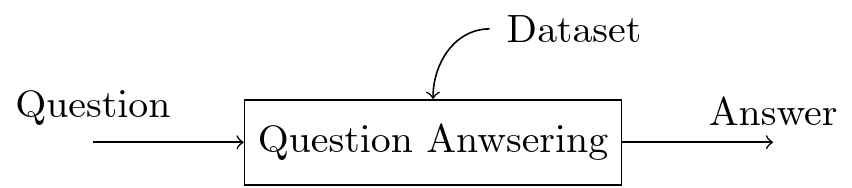
\includegraphics[width=\textwidth,height=6cm,keepaspectratio=true]{intro_qa}
    \caption{Suggested \gls{qa} diagram}
    \label{fig:intro_qa}
\end{figure}

\paragraph{Primaries}
\begin{itemize}[noitemsep]
    \item Select existing papers and projects treating the subject as a starting point.
    \item Identify relevant datasets.
    \item Develop one or more \gls{poc}.
    \item Test and evaluate solutions.
    \item Suggest improvements, possible continuation, and future outcomes.
\end{itemize}
\paragraph{Secondaries}
\begin{itemize}[noitemsep]
    \item Extended the \gls{qa} chatbot using tailored knowledge.
\end{itemize}

\subsection*{Generative \gls{qa} Chatbot}
The second objective is to improve the output from the prior objective into enhanced answers.
\begin{figure}[ht!]
    \centering
    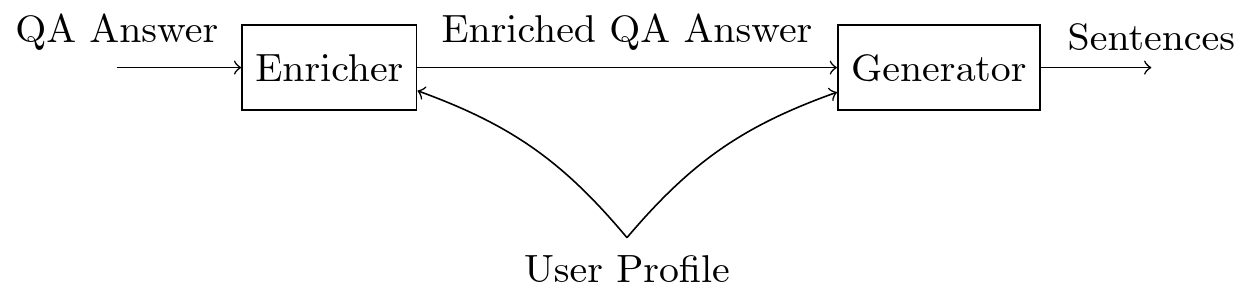
\includegraphics[width=\textwidth,height=6cm,keepaspectratio=true]{intro_qa_gen}
    \caption{Suggested Generative \gls{qa} diagram}
    \label{fig:intro_qa_gen}
\end{figure}

\paragraph{Primaries}
\begin{itemize}[noitemsep]
    \item Investigate a rule-based system for keyword enrichment.
    \item Generate sentences with keywords.
    \item Identify relevant datasets.
    \item Develop one or more \gls{poc}.
    \item Test and evaluate solutions.
    \item Suggest improvements, possible continuation, and future outcomes.
\end{itemize}
\paragraph{Secondaries}
\begin{itemize}[noitemsep]
    \item Use advanced strategies to enrich keywords.
    \item Use advanced text generation technics such as GTP-2\footnote{OpenAI's GTP-2 Algorithm\cite{papers:gpt2}}.
    \item Use user profiles to customize the outputs.
\end{itemize}


\section*{Plan}
\label{plan:plan}
\subsection*{Contraints}
\textbf{Timeframe:} 19 weeks\\
\textbf{Starting date:} 16.09.2019\\
\textbf{Ending date:} 07.02.2020

\subsection*{Methodologies}
For consistency, the project is split into two methodological parts. The first third, as the project's orientation is going toward information gathering and self-study, uses a standard sequential project management methodology. For the next two-thirds of the project, the author is using an agile methodology intending to reach incremental progress while exploring.

\subsubsection*{Back to level Milestones}
\textbf{(6 weeks)} First third of the study, from \textbf{16.09.19 to 25.10.19}.
\begin{enumerate}
    \setlength\itemsep{0em}
    \item[M1.] Initial \gls{mt} plan and project specification
    \item[M2.] Review the state of the art of the \gls{nlp} and \gls{nlu} technologies and refine the plan if needed.
\end{enumerate}


\subsubsection*{Diving into the subject Milestones}
\textbf{(13 weeks) From 28.10.19 to 07.02.20}, the following two-third of the thesis is composed 6 sprints of two weeks and one week to finalise the thesis.
\begin{itemize}
    \setlength\itemsep{0em}
    \item[M3.] Basic \gls{qa} Chatbot
    \item[M4.] Evaluation of basic \gls{qa} Chatbot
    \item[M5.] Basic generative \gls{qa} Chatbot
    \item[M6.] Evaluation of basic generative \gls{qa} Chatbot
\end{itemize}

\subsection*{Gantt}
The Figure~\ref{fig:gantt-specification} represents the chart for the initial plan.

\newganttchartelement*{specifications-milestones}{
specifications-milestones/.style={
shape=isosceles triangle,
inner sep=0pt,
draw=cyan,
top color=white,
bottom color=cyan!50
},
specifications-milestones incomplete/.style={
/pgfgantt/specifications-milestones,
draw=yellow,
bottom color=yellow!50
},
specifications-milestones label font=\slshape,
specifications-milestones left shift=0pt,
specifications-milestones right shift=0pt
}

\newgantttimeslotformat{stardate}{
\def\decomposestardate##1.##2\relax{
\def\stardateyear{##1}\def\stardateday{##2}
}
\decomposestardate#1\relax
\pgfcalendardatetojulian{\stardateyear-01-01}{#2}
\advance#2 by-1\relax
\advance#2 by\stardateday\relax
}

\begin{figure}[h]%[htbp]
\centering
\begin{ganttchart}[vgrid, hgrid]{1}{19}
\gantttitle{Sep}{2} 
\gantttitle{Oct}{5}
\gantttitle{Nov}{4}
\gantttitle{Dec}{3}
\gantttitle{Jan}{4}
\gantttitle{Feb}{1}\\
\gantttitlelist{1,...,19}{1}\\

%part 1
\ganttgroup{Back to level}{1}{6} \\
\ganttmilestone{M1, M2}{3}
\ganttmilestone{}{6}\\

%part 2
\ganttgroup{Diving}{7}{18} \\
\ganttbar{Sprint 1}{7}{8} \\
\ganttbar{Sprint 2}{9}{10} \\
\ganttmilestone{M3}{10}\\
\ganttbar{Sprint 3}{11}{12} \\
\ganttmilestone{M4}{12}\\
\ganttbar{Sprint 4}{13}{14} \\
\ganttbar{Sprint 5}{15}{16} \\
\ganttmilestone{M5}{16}\\
\ganttbar{Sprint 6}{17}{18} \\
\ganttmilestone{M6}{18}\\

%\ganttlink{elem6}{elem7}
%\ganttlink{elem8}{elem9}

%part 3
\ganttgroup{Wrap up}{19}{19} \\


\end{ganttchart}

\caption{Project Specificiation Gantt Chart}
\label{fig:gantt-specification}
\end{figure}

\cleardoublepage

% ---------------------------------------------------------------------
% STUDENT INFORMATION
% ---------------------------------------------------------------------
\frontmatter
\setcounter{page}{1}
Accepted by the HES-SO//Master (Switzerland, Lausanne) on a proposal from:

\vspace{0.5cm}

\Supervisor, deepening project supervisor

\Expert, \ExpertLab, main expert

\vspace{1cm}

Place, date: \underline{\hspace{8cm}}

\vspace{3cm}

{ \renewcommand{\arraystretch}{1.5}
\begin{tabularx}{\textwidth}{X X}
	\Supervisor  & \MRU\\
	Supervisor   & \acrshort{ict} \acrshort{mru} Leader at HES-SO//Fribourg\\
\end{tabularx}
}

% ---------------------------------------------------------------------
% DEDICATE
% ---------------------------------------------------------------------
\textbf{Dedicate}\\

To my family that believed in me, and still I don't know why.

% ---------------------------------------------------------------------
% TABLE OF CONTENTS
% ---------------------------------------------------------------------
\cleardoublepage
\phantomsection
\addcontentsline{toc}{chapter}{Contents}
\tableofcontents

% ---------------------------------------------------------------------
% ACKNOWLEDGMENTS
% ---------------------------------------------------------------------
\chapter*{Acknowledgments}
\addcontentsline{toc}{chapter}{Acknowledgments}

I wish I could thank an \gls{agi} for doing my thesis, meanwhile here follows my acknowledgments.

\section*{People}
\paragraph {Jean Hennebert} for his advice and the opportunity to work on a meaningful subject to me.
\paragraph {Fiona Baumann} For her endless support and proofreading.
\paragraph {Damien Goetschi} For his proofreading.
\paragraph {Aymeric Genêt} For his support and proofreading.
\paragraph {Jämes Ménétrey} For his advice and support.
\paragraph {Lucy Linder} For many interesting discussions and her advice.
\paragraph {Luana Martelli} For her support and proofreading.
\paragraph {Riccardo Formenti} For his advice and support.
\paragraph {The whole iCoSys team} For the social interaction and the incredible ambiance.
\paragraph {My open-space} To all my colleagues that supported me and helped me stay sane during this project.
\paragraph {My closes friends} Julia, Séverine, Jeff, Thomas, Simon, Fabián, Diane, and Marc for their support.
\paragraph {My parents} For their support.

% ---------------------------------------------------------------------
% GLOSSARY
% ---------------------------------------------------------------------
% ---------------------------------------------------------------------
% Cloned from the HES-SO//Master canvas 2019
% ---------------------------------------------------------------------
%\acrshort{mru}
%\gls{tic}

% ---------------------------------------------------------------------
% GLOSSARY
% format:  \newglossaryentry{<label>}{<settings>}
% example: \newglossaryentry{adagrad}
% ---------------------------------------------------------------------
\newglossaryentry{adagrad}
{
  name=Model,
  description={In \gls{ml}, a model is the representation of the assumptions made by the algorithm during the training phase. Models are used to output a result based on a provided input and the learning patterns.}
}
	



% ---------------------------------------------------------------------
% Acronymes
% format:  \newacronym{<label>}{<abbrv>}{<full>}
% example: \newacronym{13c}{13C}{carbon-13}
% ---------------------------------------------------------------------
\newacronym{mru}{MRU}{Master Research Units}
\newacronym{ict}{ICT}{Information and Communications Technologies}
\newacronym{ann}{ANN}{Artificial Neural Networks}
\newacronym{dnn}{DNN}{Deep Neural Networks}
\newacronym{nlp}{NLP}{Natural Language Processing}
\newacronym{nlu}{NLU}{Natural Language Understanding}
\newacronym{nlg}{NLG}{Natural Language Generation}
\newacronym{ml}{ML}{Machine Learning}
\newacronym{aiml}{AIML}{Artificial Intelligence Markup Language}
\newacronym{ai}{AI}{Artificial Intelligence}
\newacronym{agi}{AGI}{Artificial General Intelligence}
\newacronym{ani}{ANI}{Artificial Narrow Intelligence}
\newacronym{asi}{ASI}{Artificial Super Intelligence}
\newacronym{scifi}{Sci-Fi}{Science Fiction}
\newacronym{faq}{FAQ}{Frequently Asked Questions}
\newacronym{rnn}{RNN}{Recurrent Neural Network}
\newacronym{ir}{IR}{Information Retrieval}
\newacronym{dm}{DM}{Data Mining}
\newacronym{bd}{BD}{Big Data}
\newacronym{dl}{DL}{Deep Learning}
\newacronym{nn}{NN}{Neural Network}
\newacronym{snn}{SNN}{Shallow Neural Network}
\newacronym{nl}{NL}{Natural Language}
\newacronym{tf-idf}{TF-IDF}{Term Frequency-Inverse Document Frequency}
\newacronym{cbow}{CBOW}{Continuous Bag of words}
\newacronym{aws}{AWS}{Amazon Web Services}
\newacronym{dp}{DP}{Deepening Project}
\newacronym{s2s}{Seq2Seq}{Sequence to Sequence}
\newacronym{mt}{MT}{Master's Thesis}
\newacronym{poc}{POC}{Proof of Concept}
\newacronym{mvp}{MVP}{Minimum Viable Product}
\newacronym{kiss}{KISS}{Keep It Stupid Simple}
\newacronym{qa}{QA}{Question Answering}
\printglossaries
\cleardoublepage

% ---------------------------------------------------------------------
% ABSTRACT
% ---------------------------------------------------------------------
\chapter*{Abstract}
\addcontentsline{toc}{chapter}{Abstract}

We propose an innovative approach for question-answering chatbots to handle conversational contexts and generate natural language sentences as answers. In addition to the ability to answer open-domain questions, our zero-shot learning approach, which uses a pure algorithmic orchestration in a grounded learning manner, provides a modular architecture to swap statically or dynamically task-oriented models while preserving its independence to training.

In the scope of this research, we realize the proof-of-concept of an open-domain and closed-ended question-answering chatbot able to output comprehensive natural language generated sentences using the Wikidata knowledge base. 

To achieve the concept, we explore the extraction, and the use of sub-knowledge graphs from the Wikidata knowledge base to answer questions conversationally and to use the sub-graphs as context holder. Additionally, we are extracting subject-predicate-object tuples from the graph and using language models to join the SPOs and extend the answers as natural language sentences.

The proof-of-concept architecture uses a combination of state-of-the-art and industry-used models with a fine-tuning strategy. As a motivational target, we use a zero-shot learning approach, by combining various models with an algorithmic orchestrator and using pure algorithmic for the graph manipulation and answer extraction.

Finally, we evaluate the answers and compare the results with state-of-the-art single-hop and multi-hop question-answering systems on question-answering datasets. We find out that, aside from the computation time and the computational resources needed, our proof-of-concept performs similarly at question-answering compared to its competitors. 

\vskip0.5cm
\textbf{Keywords:} 
\Keywords

% ---------------------------------------------------------------------
% HOW TO READ
% ---------------------------------------------------------------------
\chapter{How to read this document}
\label{chap:how-to-read}
Describing the structure of the document with a redline and its reasoning. 

\todo{To be completed at the end of the work}

\section*{Project preface}
Introducing the project

\section*{State-of-the-art}
In this part, we will be exploring the state of the art of \gls{nlp} technologies as it is at the beginning of 2020. 

\section*{Design and realization}
Explaining how we got to build a proof of concept, what happened during the process of the initial plan, and how when came up with an innovative solution while solving and starting the design project from scratch.


\section*{Retrospective}
The results are here; it's awesome what we accomplished!

% ---------------------------------------------------------------------
% MAIN
% ---------------------------------------------------------------------
\mainmatter

% ---------------------------------------------------------------------
% CHAPTERS
% ---------------------------------------------------------------------
% PART 1
\part{Project preface}
\chapter{Introduction}
\label{chap:introduction}

New technologies are revolutionizing the way humans access knowledge as a service from multiple platforms and providers. Thanks to the emergence of increasingly powerful \gls{ai} algorithms, particularly in the field of \gls{nlp}, conversational agents, commonly named chatbots, have come a long way and have become popular among information consumers. As it is in early 2020, chatbots are all still \glspl{ani}\footnote{The State of AI Report 2019 \autocite{studies:state_of_ai_2019}}. Even if the chatbots are continually improving at providing the best outputs for specific tasks as well as providing meaningful human-like sentences, they still cannot generalize the tasks toward human-like conversations. The task of conversation, as humans are applying it, a complex integration of tasks including understanding, reasoning, context linking, context tracking, curiosity, initiatives, \gls{few-shot} or \gls{zero-shot} and learning on the fly, have yet to be accomplished. Nonetheless, as research progresses, chatbots are improving with new technics and tools that are making them step by step closer to complete human-like discussions, slowly progressing towards \gls{agi} chatbots. As for the scope of the thesis, we are humbly focusing on the combination of few \gls{nlp} tasks with a \gls{zero-shot} approach to help \gls{ml} and \gls{nlp} research getting closer to General \gls{qa} Conversational Chatbots. 

\section{Aim of the Research}
The initial goal of the thesis was to explore and combine \gls{sota} \gls{qa} Systems and \glspl{lm} to into an experimental \gls{poc} of a Conversational \gls{qa} Chatbots.

During our research journey, we discovered a new purpose to the project, and took a step into the unknown with a \gls{zero-shot} approach with sub-knowledge graphs.

\subsection{Project's Overall Scope}
We are focusing on the English language as an attempt to increase the number of compatible datasets and make community accessible solutions. We are exploring and combining two types of systems as an attempt to build \gls{qa} chatbots. The first system will produce factual answers, and the second system will generate human-like sentences from the answers found by the primary system. For the factual answers, we will be evaluating the results of our combined system against \gls{sota} \gls{qa} systems on \gls{qa} testing datasets. Humans will manually evaluate the answered sentences from our combined system. Finally, as the time allocated for the thesis is 19 weeks, the outcomes are narrowed at providing non-exhaustive research and a \gls{poc} solution. On a side note, the review of the risks and ethical problems that could be raised by the development of such solutions are not part of this work.

%\newpage

\subsection{Industrial Interest}
\textit{iCoSys}, the Institut of Complex Systems at the University of Applied Sciences and Arts at Fribourg, Switzerland, is interested in the results of this study for their \textit{AI-News} project\footnote{\url{AINews.ch}}. Its goal is to provide a chatbot-based system as a tool for press readers, to help them narrow their interests and deliver the right information. This project is in collaboration with the \textit{Swiss Innovation Agency} from the Swiss Confederation, \textit{La Liberté}, the daily newspaper from Fribourg and \textit{Djebots}, a startup selling scenario-based narrow chatbots.

\subsection{Personal Interest}
In harmony with the thesis subject, as the author is particularly interested in exploring the premises to \gls{agi} related technologies such as \gls{zero-shot}, \gls{gl}, Machine Understanding, and Machine Reasoning for a Multi-Domain Task Generalization. The human-like \gls{qa} frame of this project is particularly motivational.

\section{Research Questions}
We articulate here the initial set of questions as a driver to our research work. From these questions are declined objectives, and from objectives are declined milestones framing the plan.

\begin{itemize}[noitemsep]
    \item What are the components to make \gls{qa} chatbots?
    \begin{itemize}[noitemsep]
        \item What is the \gls{sota} of chatbots and \gls{qa} systems?
        \item How to tune \gls{qa} chatbots to make them as human-like as possible?
        \item How to tune such systems for the field of journalism?
    \end{itemize}
    \item What is the state of the art for \gls{generative} \gls{qa} chatbots?
    \begin{itemize}[noitemsep]
        \item What are the components to make \gls{generative} \gls{qa} chatbots?
        \item Are \gls{generative} chatbots only as good as the data they consume?
        \item Could \gls{generative} chatbots be a step toward \gls{agi}?
    \end{itemize}
\end{itemize}

    %\item Are Knowledge-based Systems useful for \gls{qa} systems?
    %\begin{itemize}[noitemsep]
    %\item Are Knowledge Bases / Knowledge Graphs a  for \gls{qa}?
    %\end{itemize}


\cleardoublepage

% PART 2
\part{State-of-the-art}
\chapter{Chatbots}
\label{chap:chatbots}

Based on latest MMC's state of AI report\footnote{The State of AI 2019: Divergence \autocite{report:Kelnar2019}}, it appears that 26\% of the AI-Startups studied by Gartner\footnote{2'791 European AI Startups from the 2019 CIO Survey: CIOs Have Awoken to the Importance of AI \autocite{online:gartner_2019_ai_survey}} are using or making chatbots (see Figure~\ref{fig:fig_mmc_state_of_ai_2019_gartner_cio_survey_31}). The same study, made a year earlier, in 2018, shows that chatbots are not present as an application, which implies that either chatbots were not referenced as AI or that their popularity exploded within a year.\\

As it is at the beginning of 2020, based on The State of AI Report 2019 \autocite{studies:state_of_ai_2019} and the two previously mentioned studies, chatbots are commonly present but limited to narrow tasks. In most cases, they are scenario-based with sequences of if-else conditions that we classify as non-learning \gls{ai}. Moreover, hard-coded scenarios are requiring an infinite amount of human power to create generic Chatbots able to maintain a conversation at a human level. However, progress in the field of \gls{ml} and \gls{nlp} is demonstrating that providing large corpora to an unsupervised algorithm is enough to maintain a passive conversation with users, which results into a shifting of the human power into data engineering. Increasingly complex algorithms and techniques are emerging at a monthly in the field, demonstrating a trend towards conversational performance improvements. Note that even if they are getting better at providing meaningful sentences, current Chatbots are still not able to orchestrate the generalization of all the tasks required to a human-like conversation. E.g., such as understanding and reasoning based on the context, initiatives to search and learn for missing information, initiate dialogue in a meaningful manner, intuition, and much more. As a side note, the generalization of those tasks would reduce the steps significantly towards general Chatbots.\\

From a user-centric point of view, chatbots are currently trending and rising global interest for various reasons. Big companies such as \textit{Google} or \textit{Apple} are believing in the technology and are making a lot of effort at pushing the chatbots into the mainstream. Even if the word \say{chatbot} is commonly used as a buzzword without a proper definition, people have at least a mental representation of its concept. Indeed, whether they call it \say{Digital Assistant}, \say{Siri}, \say{ok Google} or \say{Alexa}, they all expect to a more or less human-like conversations after using those triggering keywords.\\

It is interesting to note that the majority of the following sections could be included in the field of \gls{ai} in general. The extrapolation of the chatbot subject to \gls{ai} as a whole is worth further studying, but it not part of this work. Instead, the focus of this chapter is Chatbots; we provide a synthesis and classification of the different methods used to build chatbots. We will define the main categories identified and continue on the main sub-categories and conclude with a cartographical chart of our chatbot vision.


%\clearpage

\begin{figure}
    \centering
    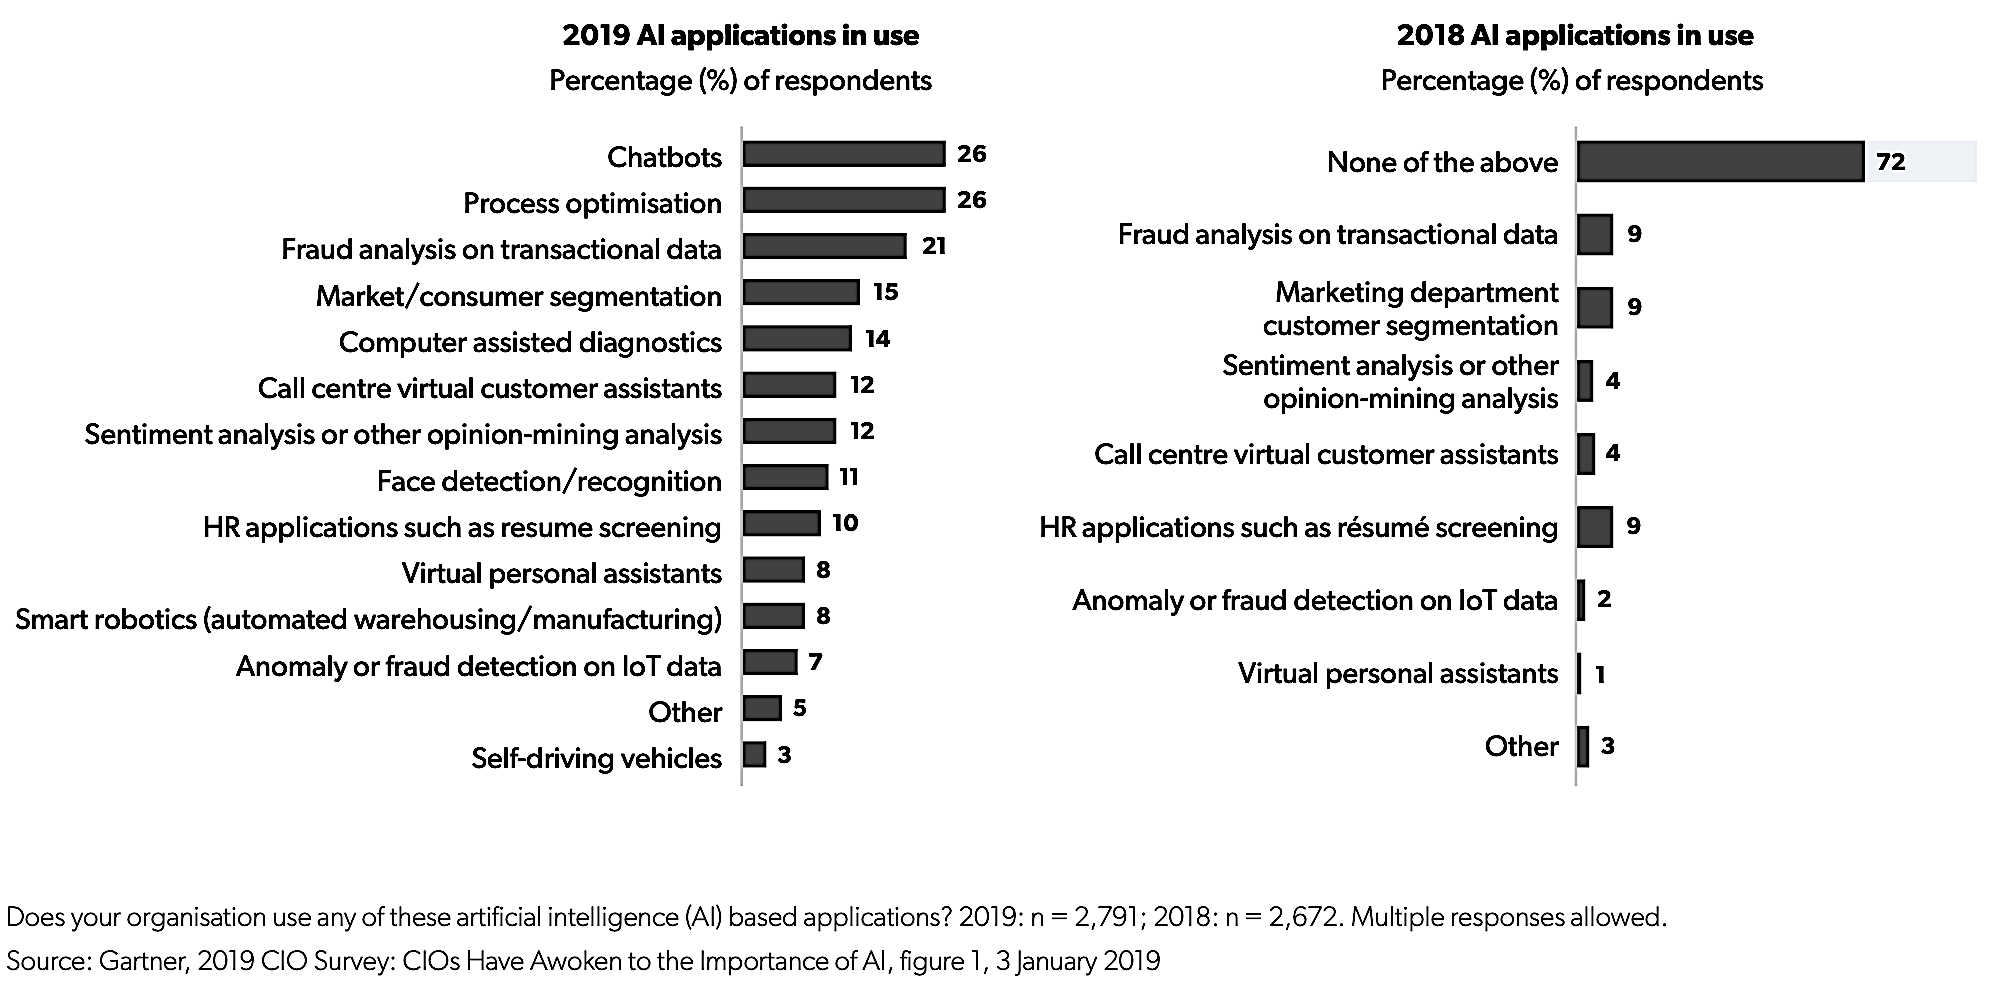
\includegraphics[width=\textwidth,keepaspectratio=true]{fig_mmc_state_of_ai_2019_gartner_cio_survey_31}
    \caption{Figure 31 from \textit{The State of AI 2019: Divergence \autocite{report:Kelnar2019}}. The top \gls{ai} applications used in European AI Startup in 2019 are Chatbots and Process optimization.}
    \label{fig:fig_mmc_state_of_ai_2019_gartner_cio_survey_31}
\end{figure}



\section{Chatbot History}
\label{chatbot:history}
Not mentioning \textit{Alan Turing} or \textit{Joseph Weizenbaum}, both considered as the fathers of \gls{ai} and chatbots, would not be fair to this research. Indeed, in 1950 they forecasted human-like communication with computers and proposed a test to differentiate humans from machines, the Turing Test \autocite{paper:turing}. The test performs as follows: a supervisor asks a human to talk to a masked entity and determine rather he is talking to a human or a computer. If the human cannot recognize speaking to a computer, then the machine passes the Turing test.\\

In 1966,\textit{Joseph Weizenbaum} wrote Eliza\autocite{website:eliza}, a computer program simulating a psychotherapist, it is seen today as one of the first well-documented attempts to make a Chatbot designed at passing the Turing test. However, due to techniqueal restrictions, Eliza was not performing particularly well in all contexts. As for today, it is still possible to play with the chatbot on a dedicated website.\\

Since Eliza, a lot of progress has been made until 2020, From conditional IF-ELSE, \gls{aiml}, up to \gls{ml} with \gls{ann} and \gls{dnn}, the improvements in the field of chatbots increased drastically over the years. Each iterations delivering algorithms being continuously more sophisticated and better at using the \gls{nl}, resulting in a new field of \gls{ml} called \gls{nlp}. As a reminder of the chatbots history and progress from 1966 to 2016, the  infographic\autocite{online:futurism_history_infography} from Futurism is particularly speaking. 


\section{Main Categories in the Chatbot Realm}
\label{chatbot:main-cats}
While performing the state-of-the-art, we identified three main chatbots categories. 

\subsection{Conversational}
We like to call them the Chatty bots, and they are great for interaction and structured replies, well designed for their ability to talk. E.g., \textit{User}: \say{Hello, how are you?}, \textit{Bot}: \say{Good, what about you?}.

\subsection{Task-Oriented}
The Task-Oriented bots are performing particularly well at specific tasks as smart-assistants. As their design is not toward generalization, their abilities are limited and will fail at off-tasks. A common workflow used by those bots is to detect the Intent and the Entities of the user request, often in \gls{nl}, then apply a rule-based matching to perform the command intended by the user. E.g., \textit{User}: \say{Book the next flight to Geneva from Zürich.}, \textit{Bot}: \say{Alright! Your ticket number is 00XXYYZZ. Have a great flight!}

\subsection{Dispatcher}
The dispatcher acts as a middleware, who's unique job is to categories the user input and forward the input to the task executor from any of the previous two categories that the user requested. E.g., If the user request the following "What is the weather in Geneva?", the dispatcher will categories the question as the task of providing the weather and sent it to the weather module. As a second example, if the user provides the following input "Hey! Let's talk about random stuff!", the dispatcher will forward the request to the chatty module.


%\clearpage

\section{Retrieval Chatbots}
\label{chatbot:retrieval}
As it is today, Retrieval-based Chatbots are popular in the industry. Indeed, a lot of tools are available, and they perform well for specific tasks. However, the response capabilities are limited to their databases and the retrieval algorithm used. Indeed, for a given input, the system is using heuristics to find the best output from the pre-defined responses. The choice of the algorithms is wide and depends on the task the chatbot is required to perform. Regardless of the heuristic used, from keywords matching up to \gls{dl}, the output will always be retrieved from the database. Concerning the database itself, the data needs a pre-processing step to generate indexes linking the questions, answers, and apply pre-calculated scores. Pre-processing also implies that if the database is updated, a new pre-processing batch is required, which implies that the scalability or fine-tuning if compromised in the long run. We like to call this type of chatbots \say{Keywords-based}. See Figure ~\ref{fig:fig_retrieval_chatbot}.

\begin{figure}
    \centering
    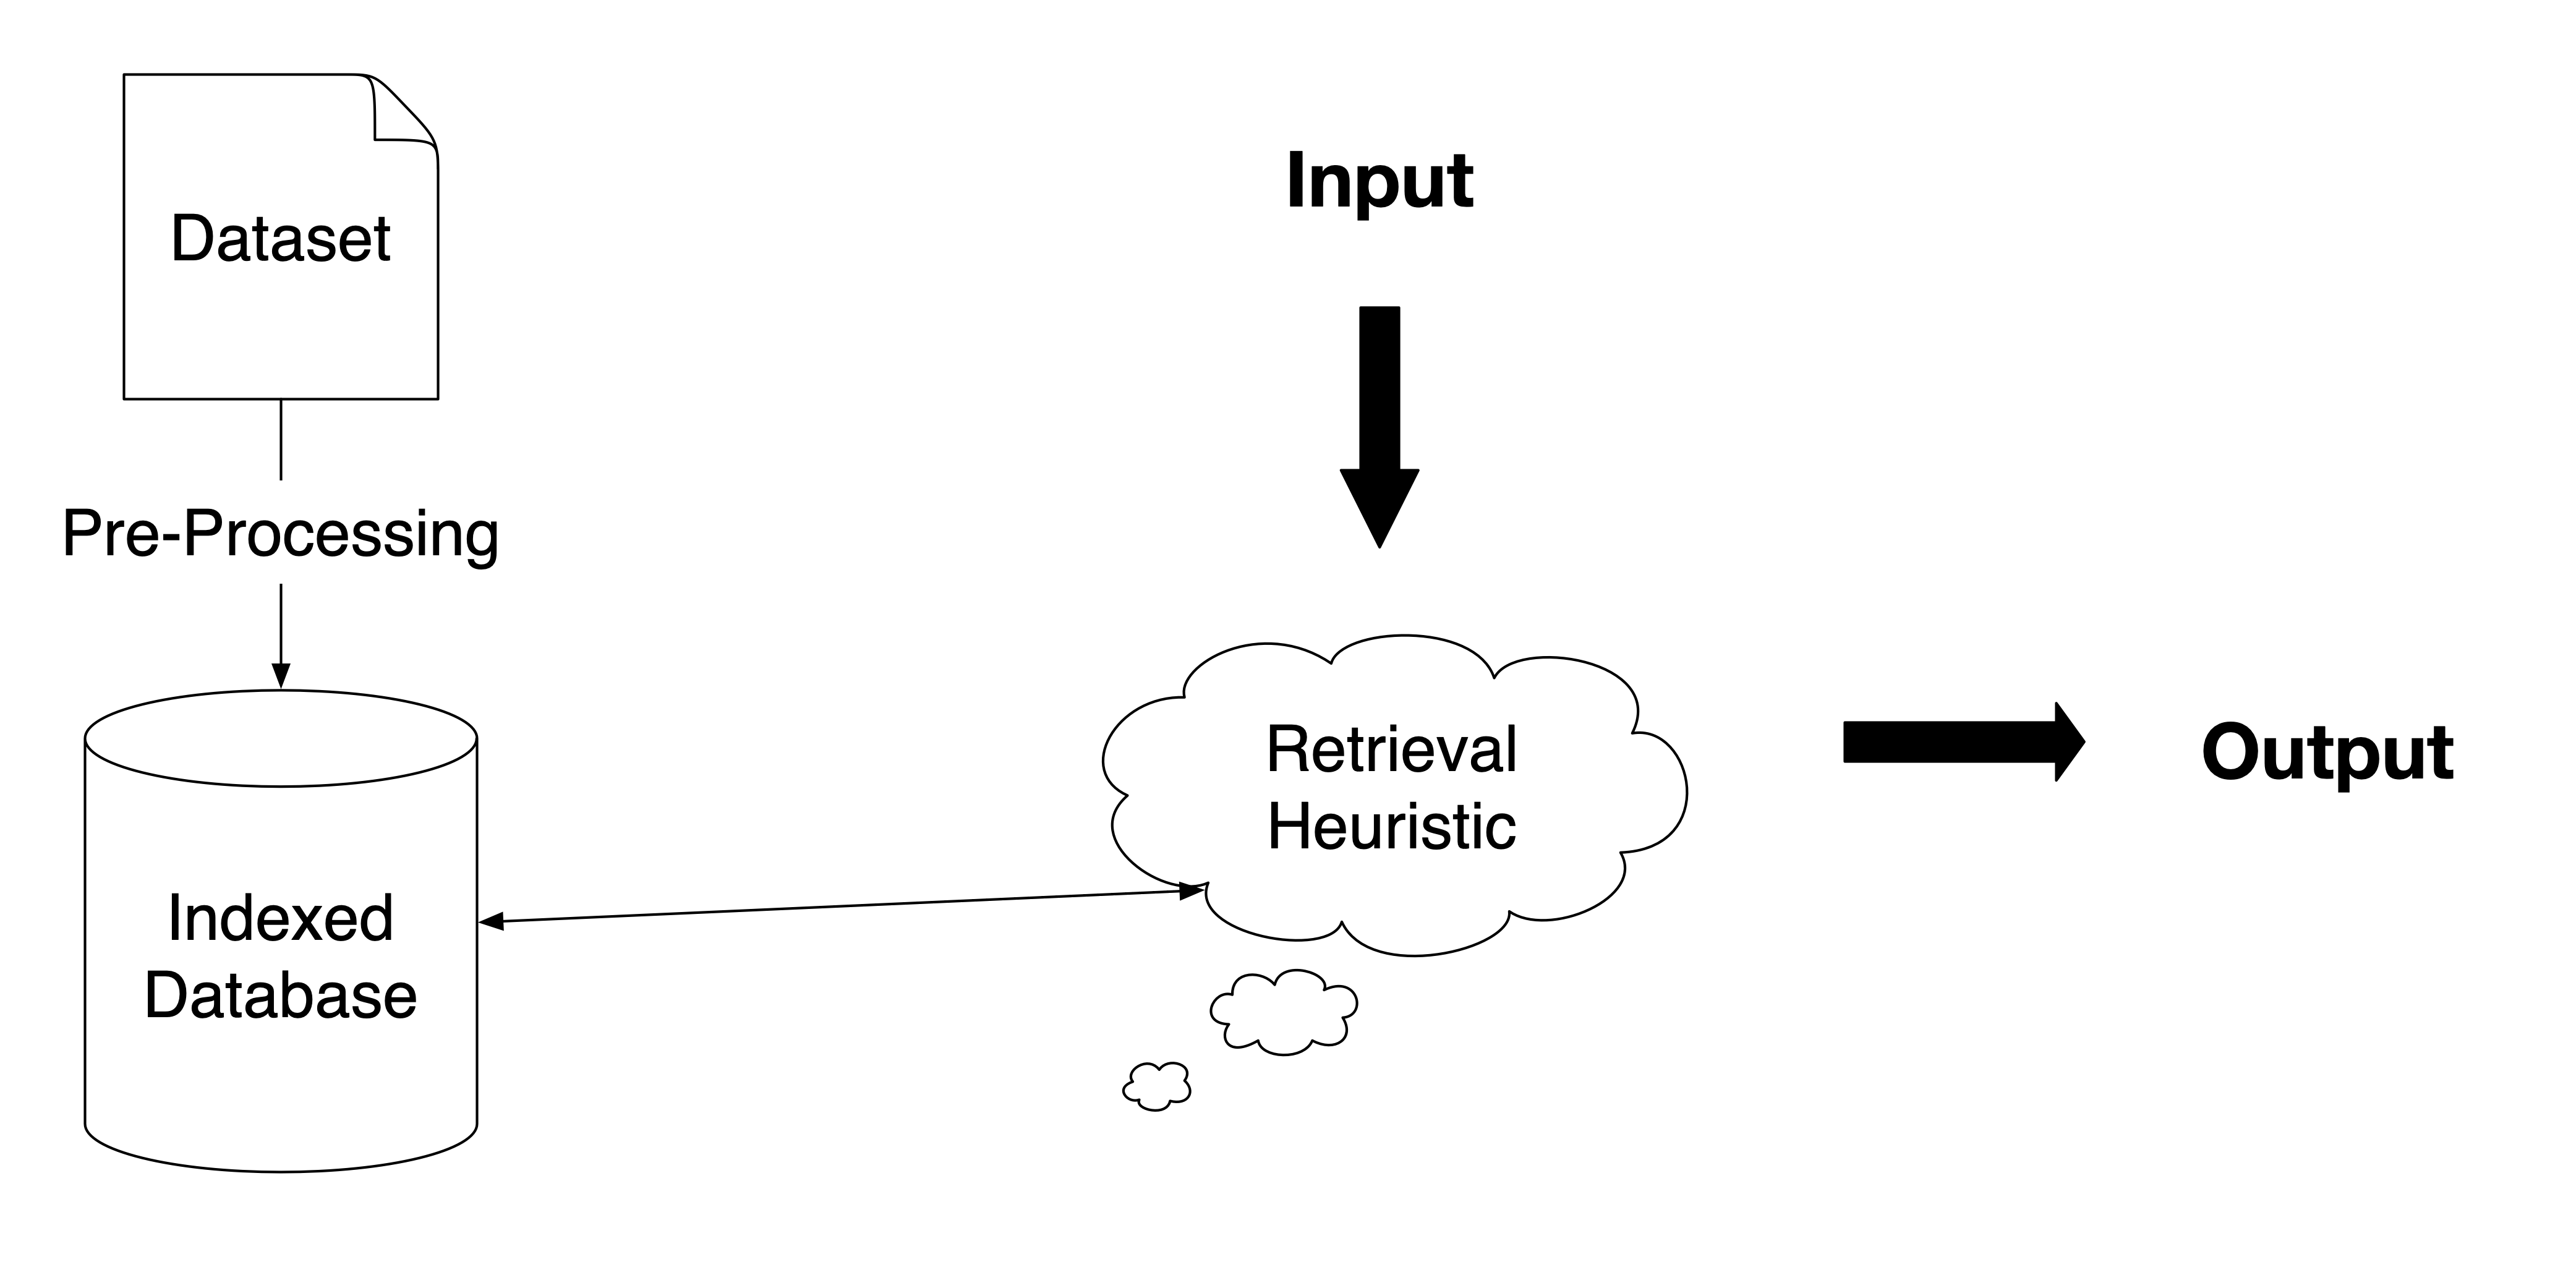
\includegraphics[width=\textwidth,keepaspectratio=true]{fig_retrieval_chatbot}
    \caption{Illustrative representation of frequent retrieval chatbots architecture.}
    \label{fig:fig_retrieval_chatbot}
\end{figure}


\section{Rule-Based Chatbots}
\label{chatbot:rulebased}
\say{Scenario-based}, as we name it, is the oldest and relatively straightforward system for chatbots. The Eliza\cite{website:eliza} Chatbot, as mentioned in the Chatbot History \ref{chatbot:history}, is scanning the input text for keywords, calculates a ranking for each keyword, and finally goes through a series of conditions called rules, and some randomness to reach the best ending leaf. Usually, the bot also includes a default output if the matching process fails, which we can still nowadays see in chatbots: \say{Hmm, this is interesting, tell me more.}. Such bots are often used for interactive chatbots, as it can, in a controlled environment, give a sense of deep meaning in the context of the conversation. Note that such systems require a lot of human power to build a frame for the bot to play in, and by this mean makes rule-based chatbots great for the specific scenario but is hard particularly hard to generalize. See Figure ~\ref{fig:fig_rulebased_chatbot}.

\begin{figure}
    \centering
    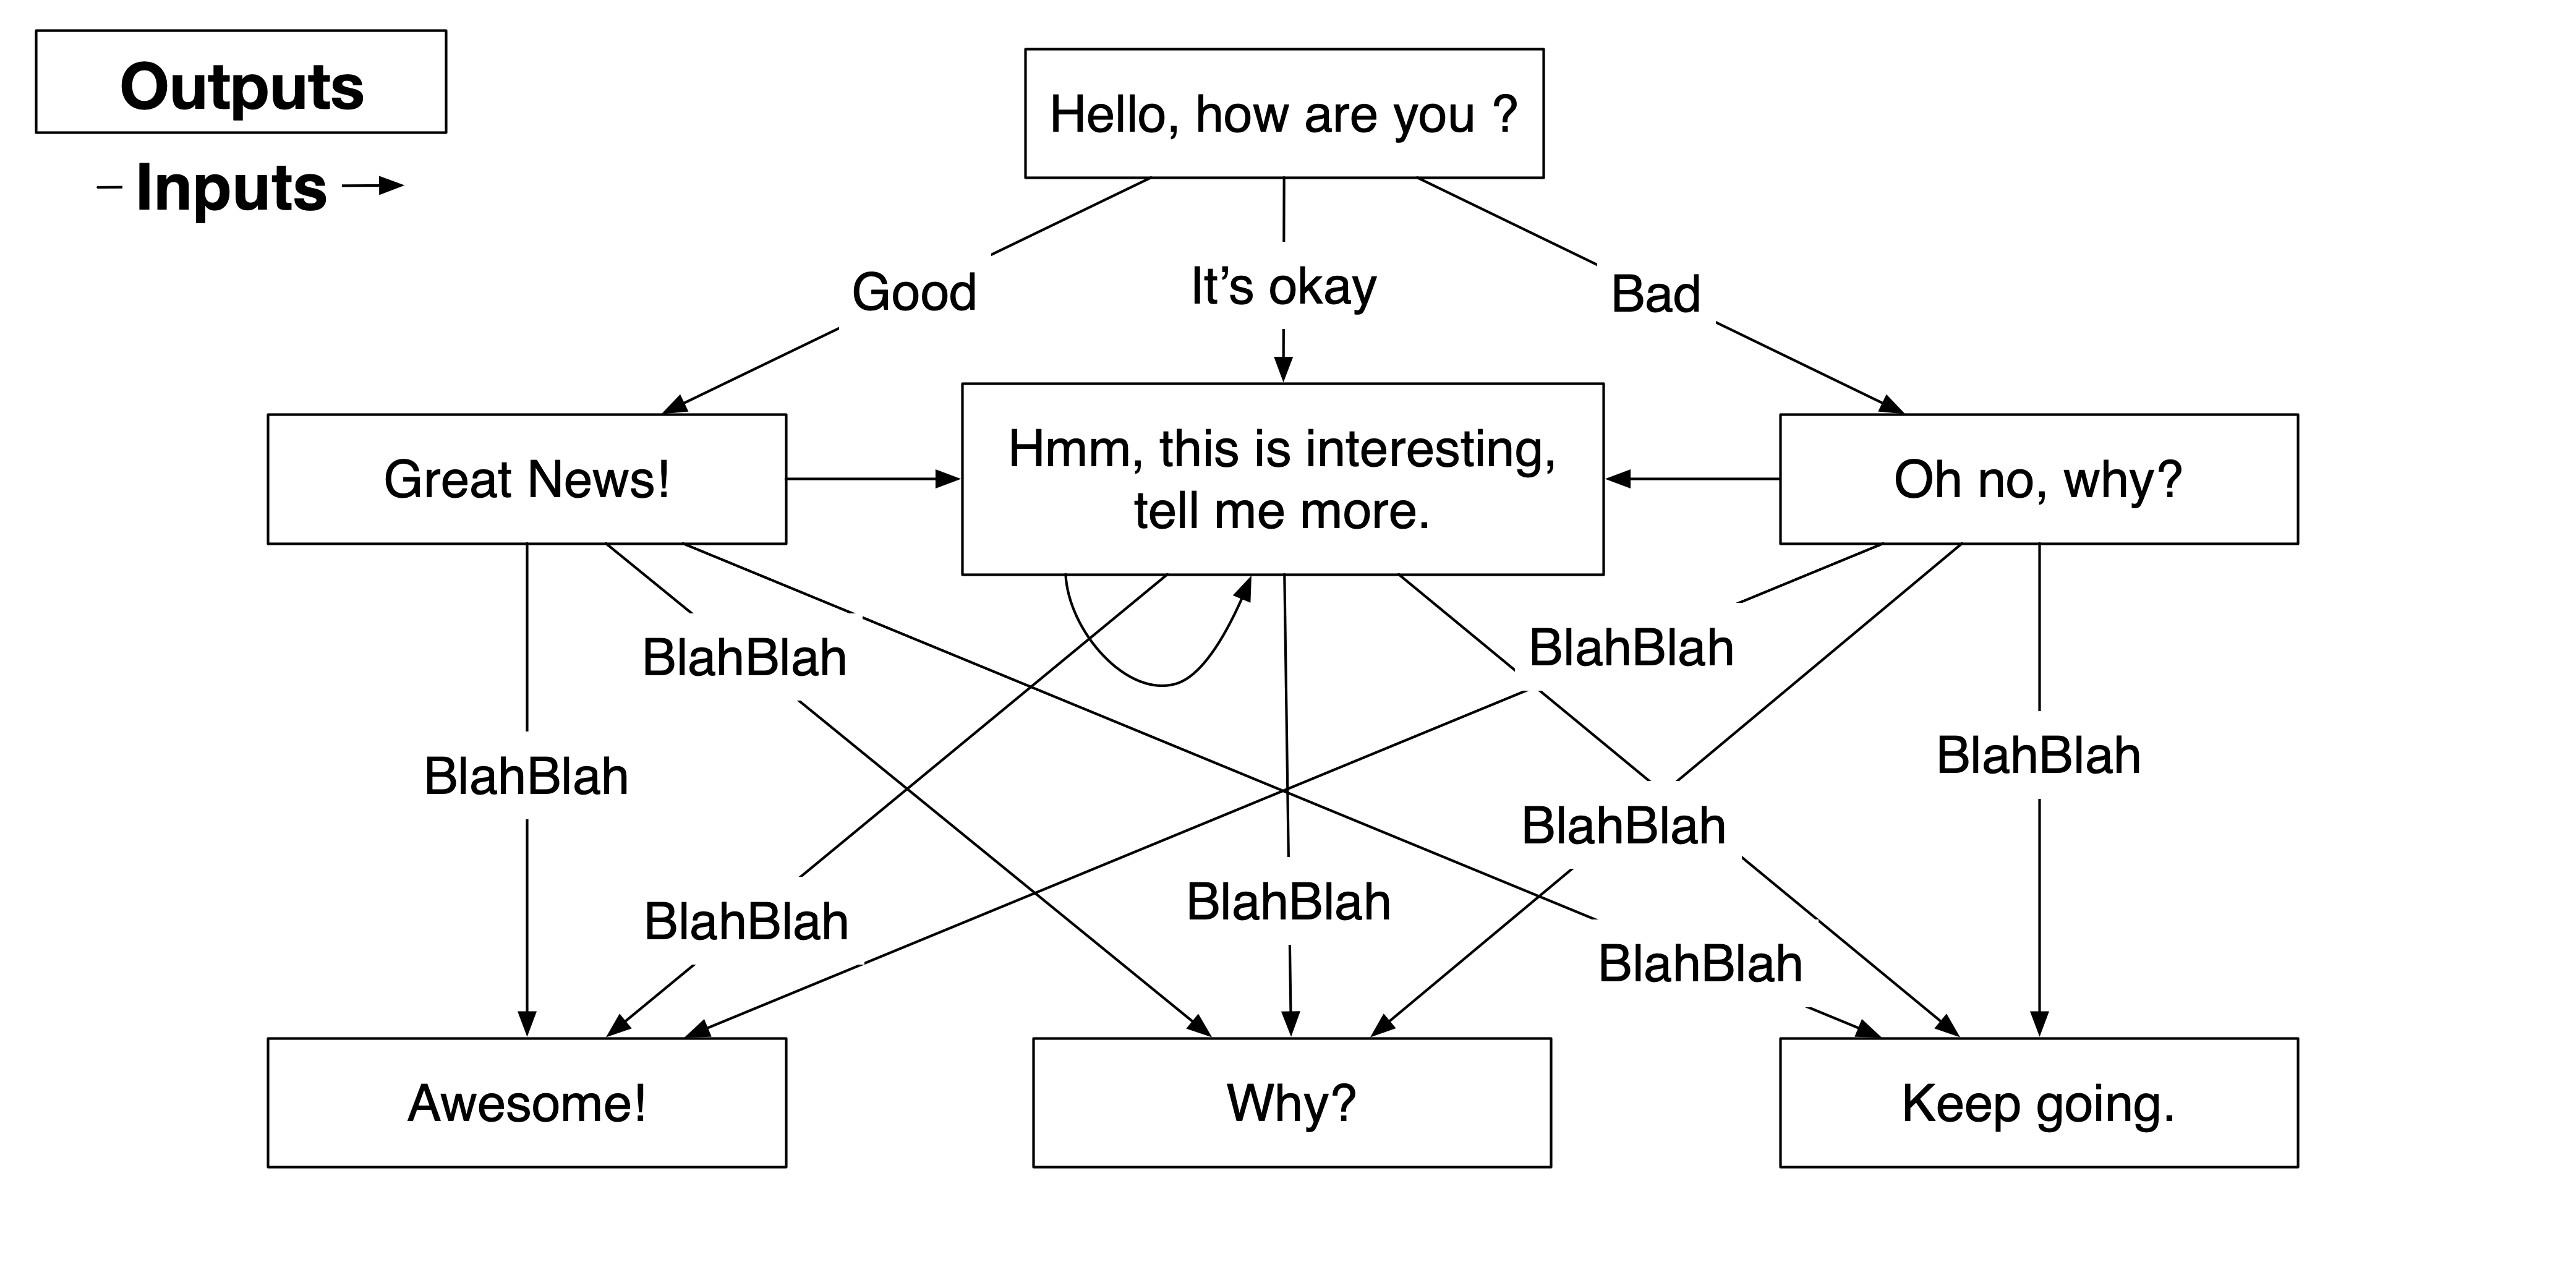
\includegraphics[width=\textwidth,keepaspectratio=true]{fig_rulebased_chatbot}
    \caption{Illustrative representation of frequent rule-based chatbots process.}
    \label{fig:fig_rulebased_chatbot}
\end{figure}

\section{Generative Chatbots}
\label{chatbot:generative}
As the current result of all the incredible innovations made in the past years in \gls{nlp}, and is a premise to true conversational chatbots, generative methods are overcoming the limitations of the Retrieval \ref{chatbot:retrieval} and Rule-Based \ref{chatbot:rulebased} Chatbots, by its ability to generate new content. Either Supervised \ref{chatbot:supervised}, Unsupervised \gls{ul} or Adversarial \ref{chatbot:adversarial}, no pre-defined outputs are used, the models are trained on large corpora to learn the language patterns and outputs relatively meaningful responses to give inputs. Another particularity of generative chatbots, is that building a domain-oriented chatbot does not require the engineers to have the domain expertise, as the expertise is embedded into the data, which allows a relative scalability to new domains. However, even if the trained models can output responses at nearly no timespan, the data-engineering of the datasets and the training phase is most often long and complicated. As a final note, the responses generated by such chatbots are only as good as the data it was fed during the training.

\subsection{Supervised Learning}
\label{chatbot:supervised}
\gls{sl} is probably the most common method used by Generative Chatbots, as it provides relative control over training. \gls{seq2seq} is commonly used as architecture for those chatbots, a \gls{nlp} version of the \gls{enc-dec}, which encodes the input words sequence and decode it into a words sequence as an answer into a framed conversation fashion. The training only requires a dataset containing a sentence and its desired response, the model will then map similar inputs with similar outputs. However, a clear limitation for this learning is that the model will for any input always have an answer, regardless of the overall meaning. Additionally, \gls{seq2seq} will prioritize the highest word apparition probabilities, meaning that data duplicates and requiring sentences will create a trend during decoding. E.g., \say{I don't know the answer.}. See Figure ~\ref{fig:fig_supervised_chabots} 

\begin{figure}
    \centering
    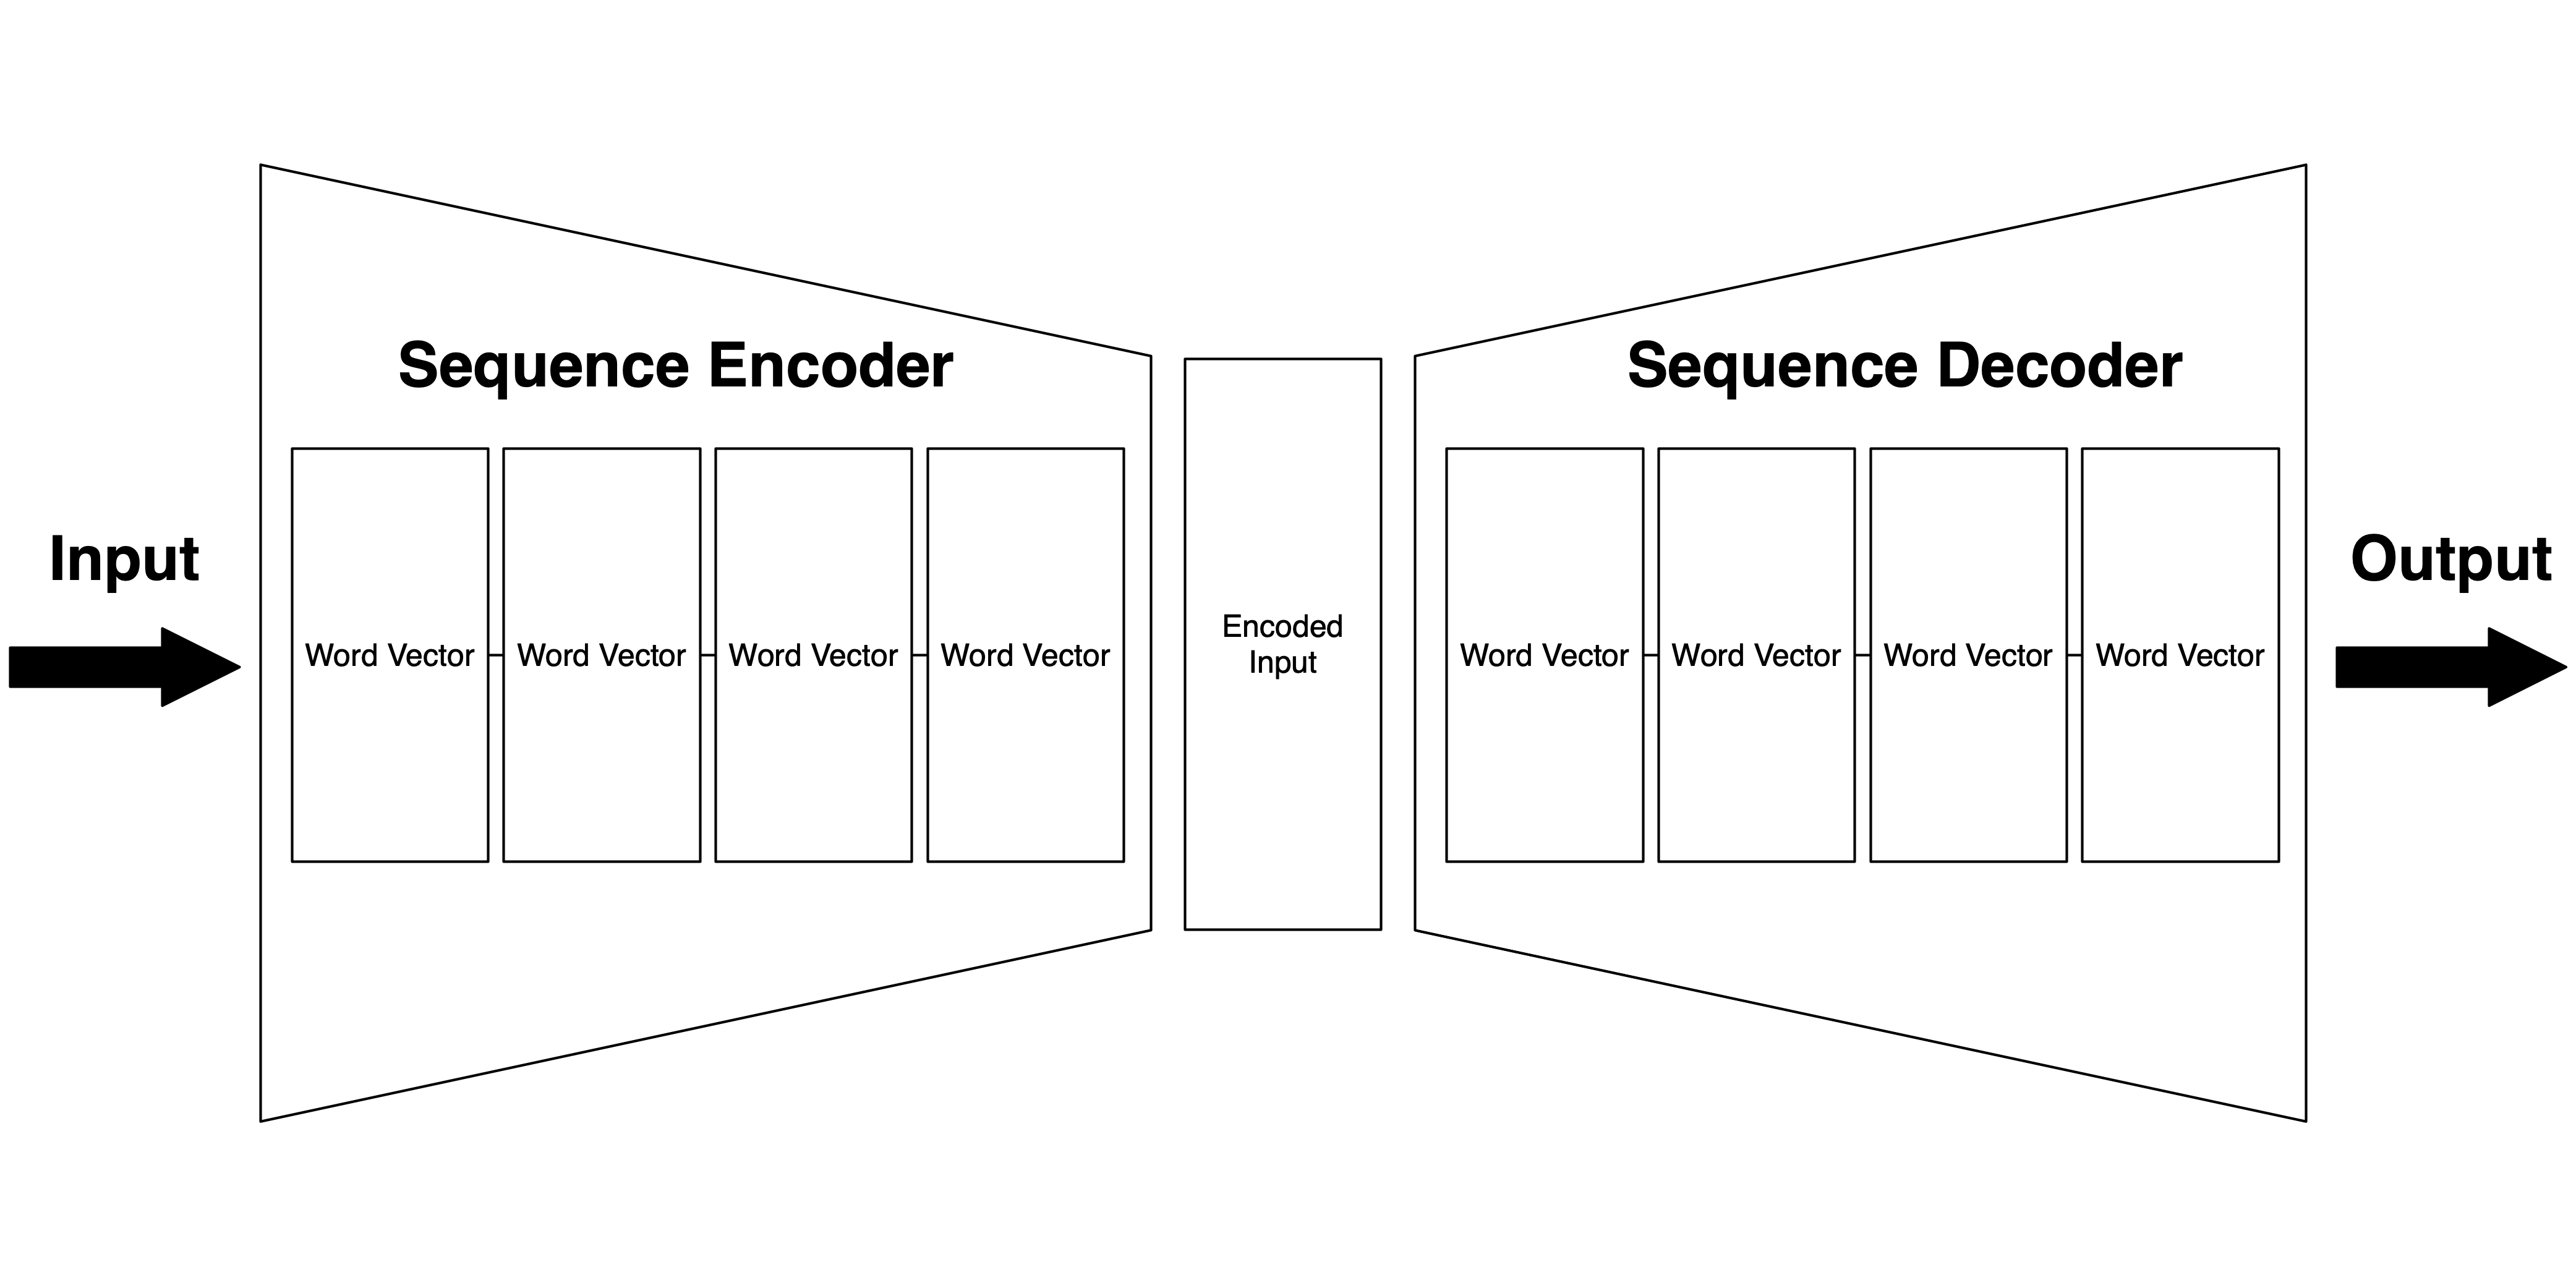
\includegraphics[width=\textwidth,keepaspectratio=true]{fig_supervised_chabots}
    \caption{Illustrative representation of a Sequence to Sequence architecture.}
    \label{fig:fig_supervised_chabots}
\end{figure}

\subsection{Adversarial Learning}
\label{chatbot:adversarial}
\gls{al} has driven attention thanks to Computer Vision \gls{gan} \autocite{paper:Karras2019stylegan2} by proving that it is possible to generate realistic human faces \autocite{website:person_does_not_exist}. In the chatbots context, it can be extrapolated into a futuristic version of the Turing Test \ref{chatbot:history}, in which machines are confronting themselves instead of humans. The concept implies the use of a training dataset containing human conversations, and compare them against the generated answer; the discriminator will then judge which is from a human and which is from an algorithm. Note that adversarial methods such as \gls{gan} are working well because of the nature of the data it plays with; indeed, pixels can be deeply noised, but words cannot be due to their discrete nature. See Figure ~\ref{fig:fig_adversarial_chatbots} 

\begin{figure}
    \centering
    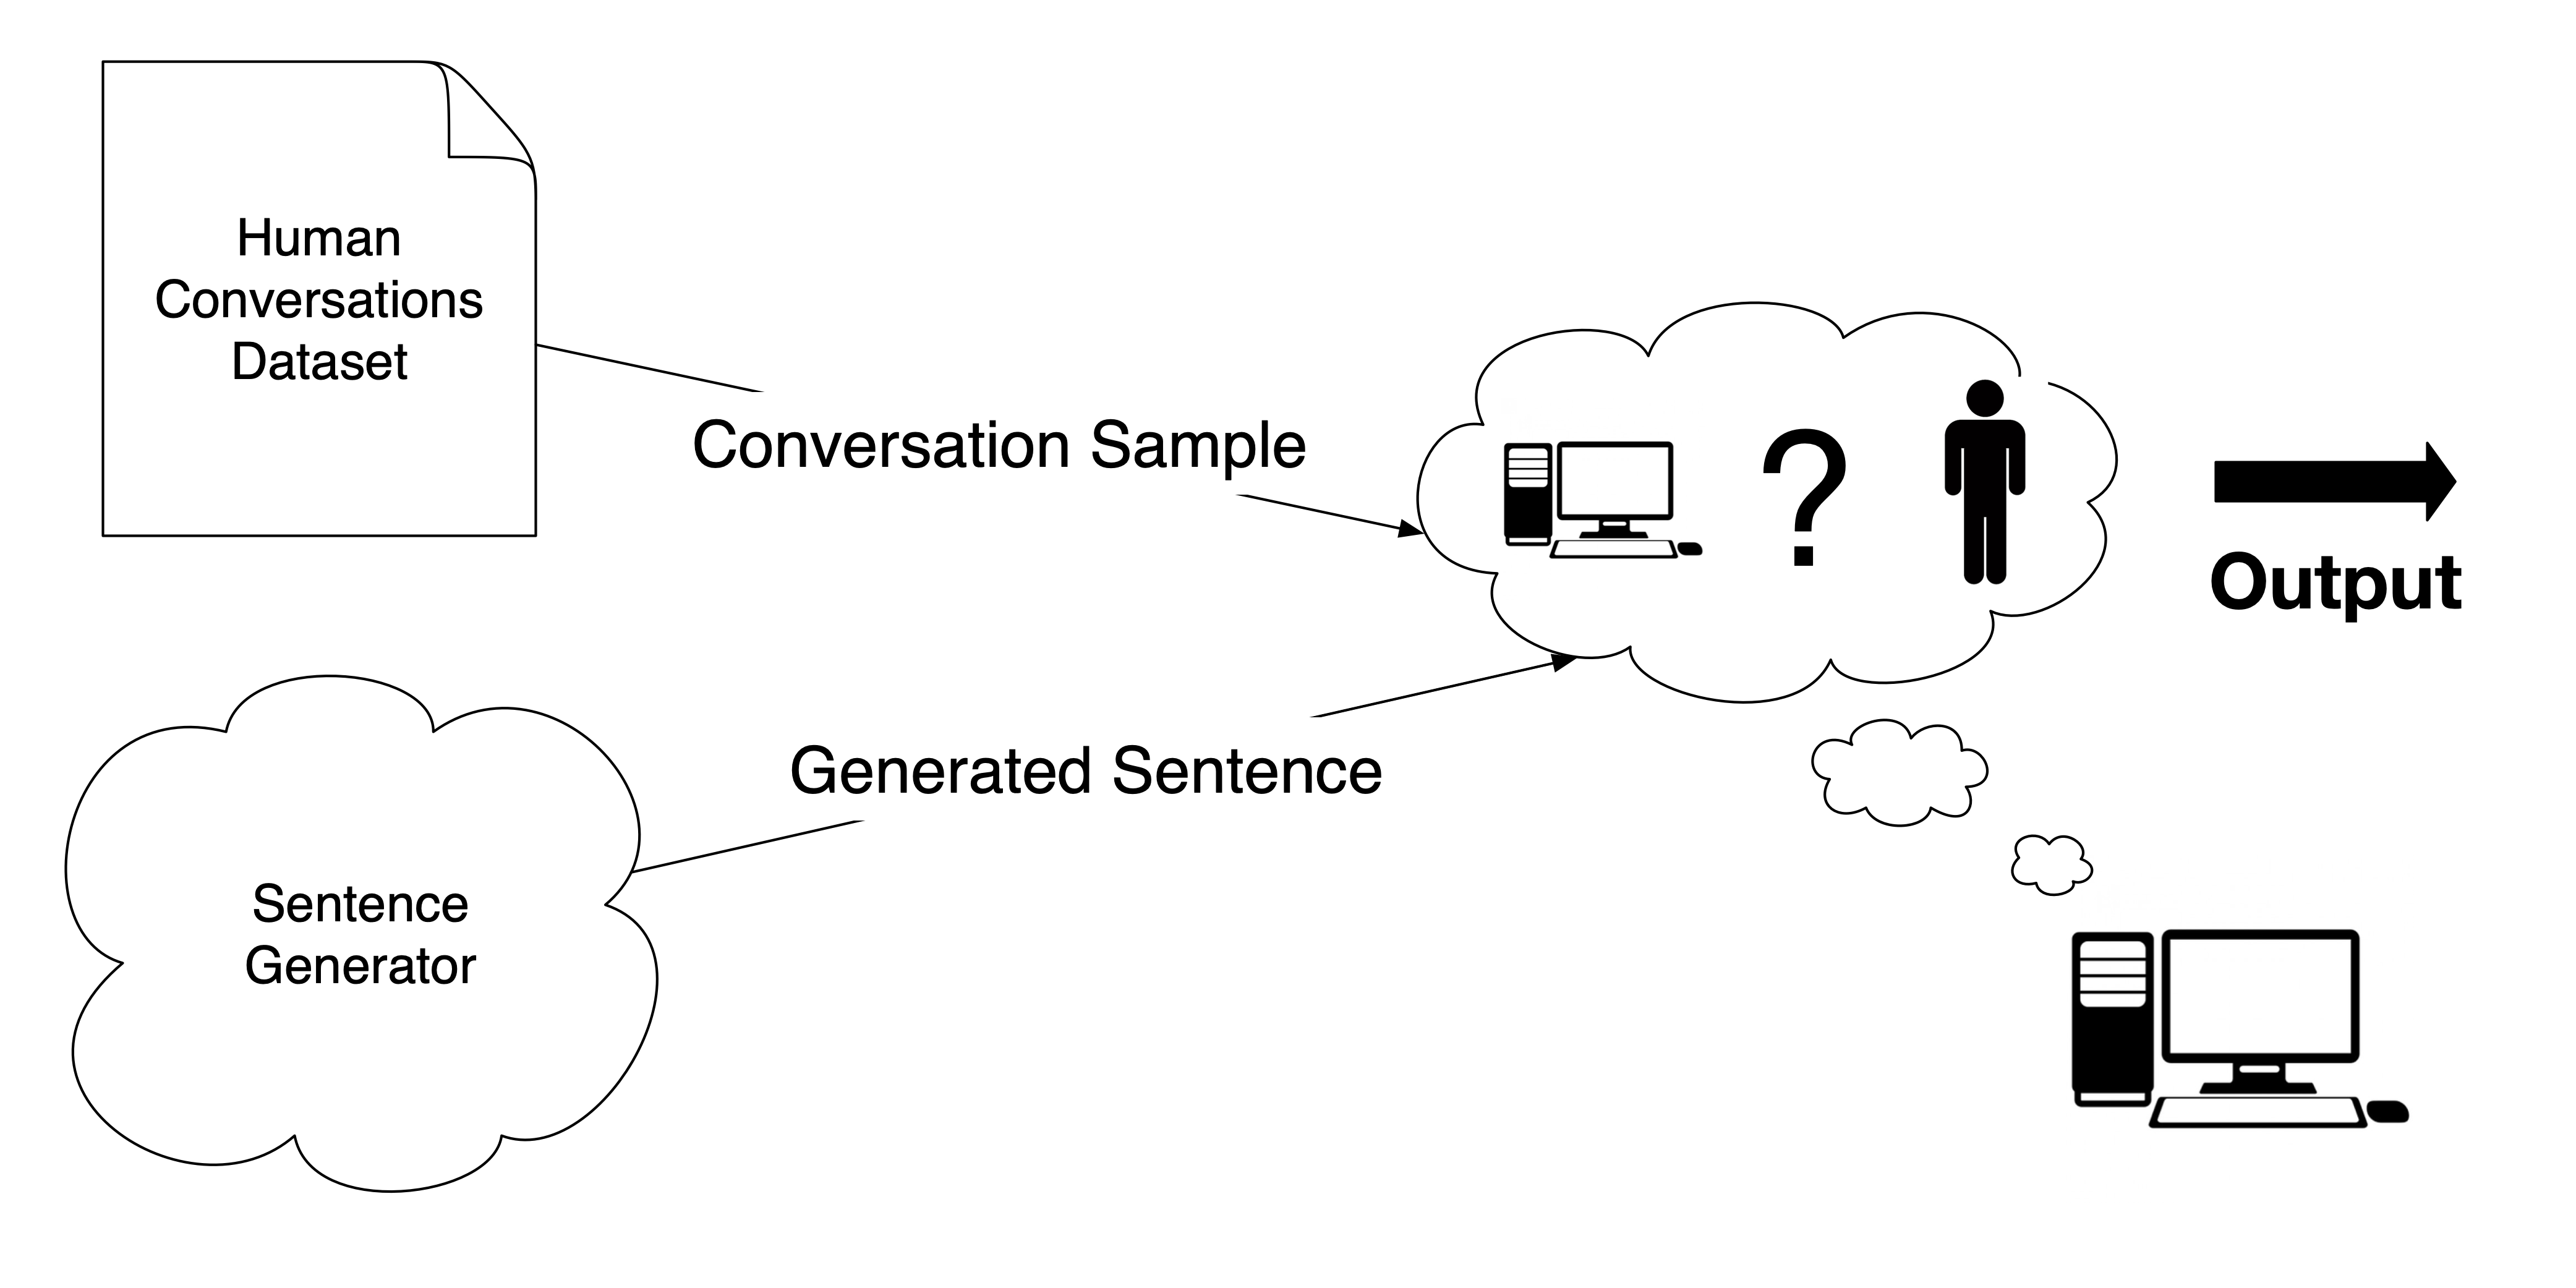
\includegraphics[width=\textwidth,keepaspectratio=true]{fig_adversarial_chatbots}
    \caption{Illustrative representation of an adversarial architecture in a chatbot context.}
    \label{fig:fig_adversarial_chatbots}
\end{figure}

\subsection{Pre-trained Language Models}
Language Models are currently the most recent and the most promising models due to their ability to model language itself instead of conversations and then tune the outputs as a chatbot would. It can been seen as semi-supervised learning, as it uses \gls{ul} for training and supervised learning \ref{chatbot:supervised} for fine-tuning \ref{chatbot:finetuning}. We will dive into \gls{lm} in the \gls{nlp} chapter \ref{nlp-lm}.

\subsection{Model Fine-Tuning}
\label{chatbot:finetuning}
With \gls{model-ft} (see Figure ~\ref{fig:fig_finetunedmodel_chatbots}), \gls{lm} have, by design, the ability to be enhanced to perform particularly a various \gls{nlp} task such as chatbots. Because pre-trained \glspl{lm} are based on the grounded blocks of language itself, implying model post-training customization as a light learning task. Indeed, it is relatively easy to fine-tune a \gls{qa} dataset to a \gls{lm}, making the model able to answer questions instead of descriptively filling sentences. The main downside to those models is the large memory size required to run them. However, due to their nature, they are trained once and then fine-tuned. Note that training requires an enormous amount of computational power. E.g, The largest form of BERT \autocite{paper:devlin-etal-2019-bert} was trained on 16 TPUs for 4 days. Fine-tuning, on the other hand, scales down to few hours on a single TPU, which makes it relatively scalable to new domains.

\begin{figure}
    \centering
    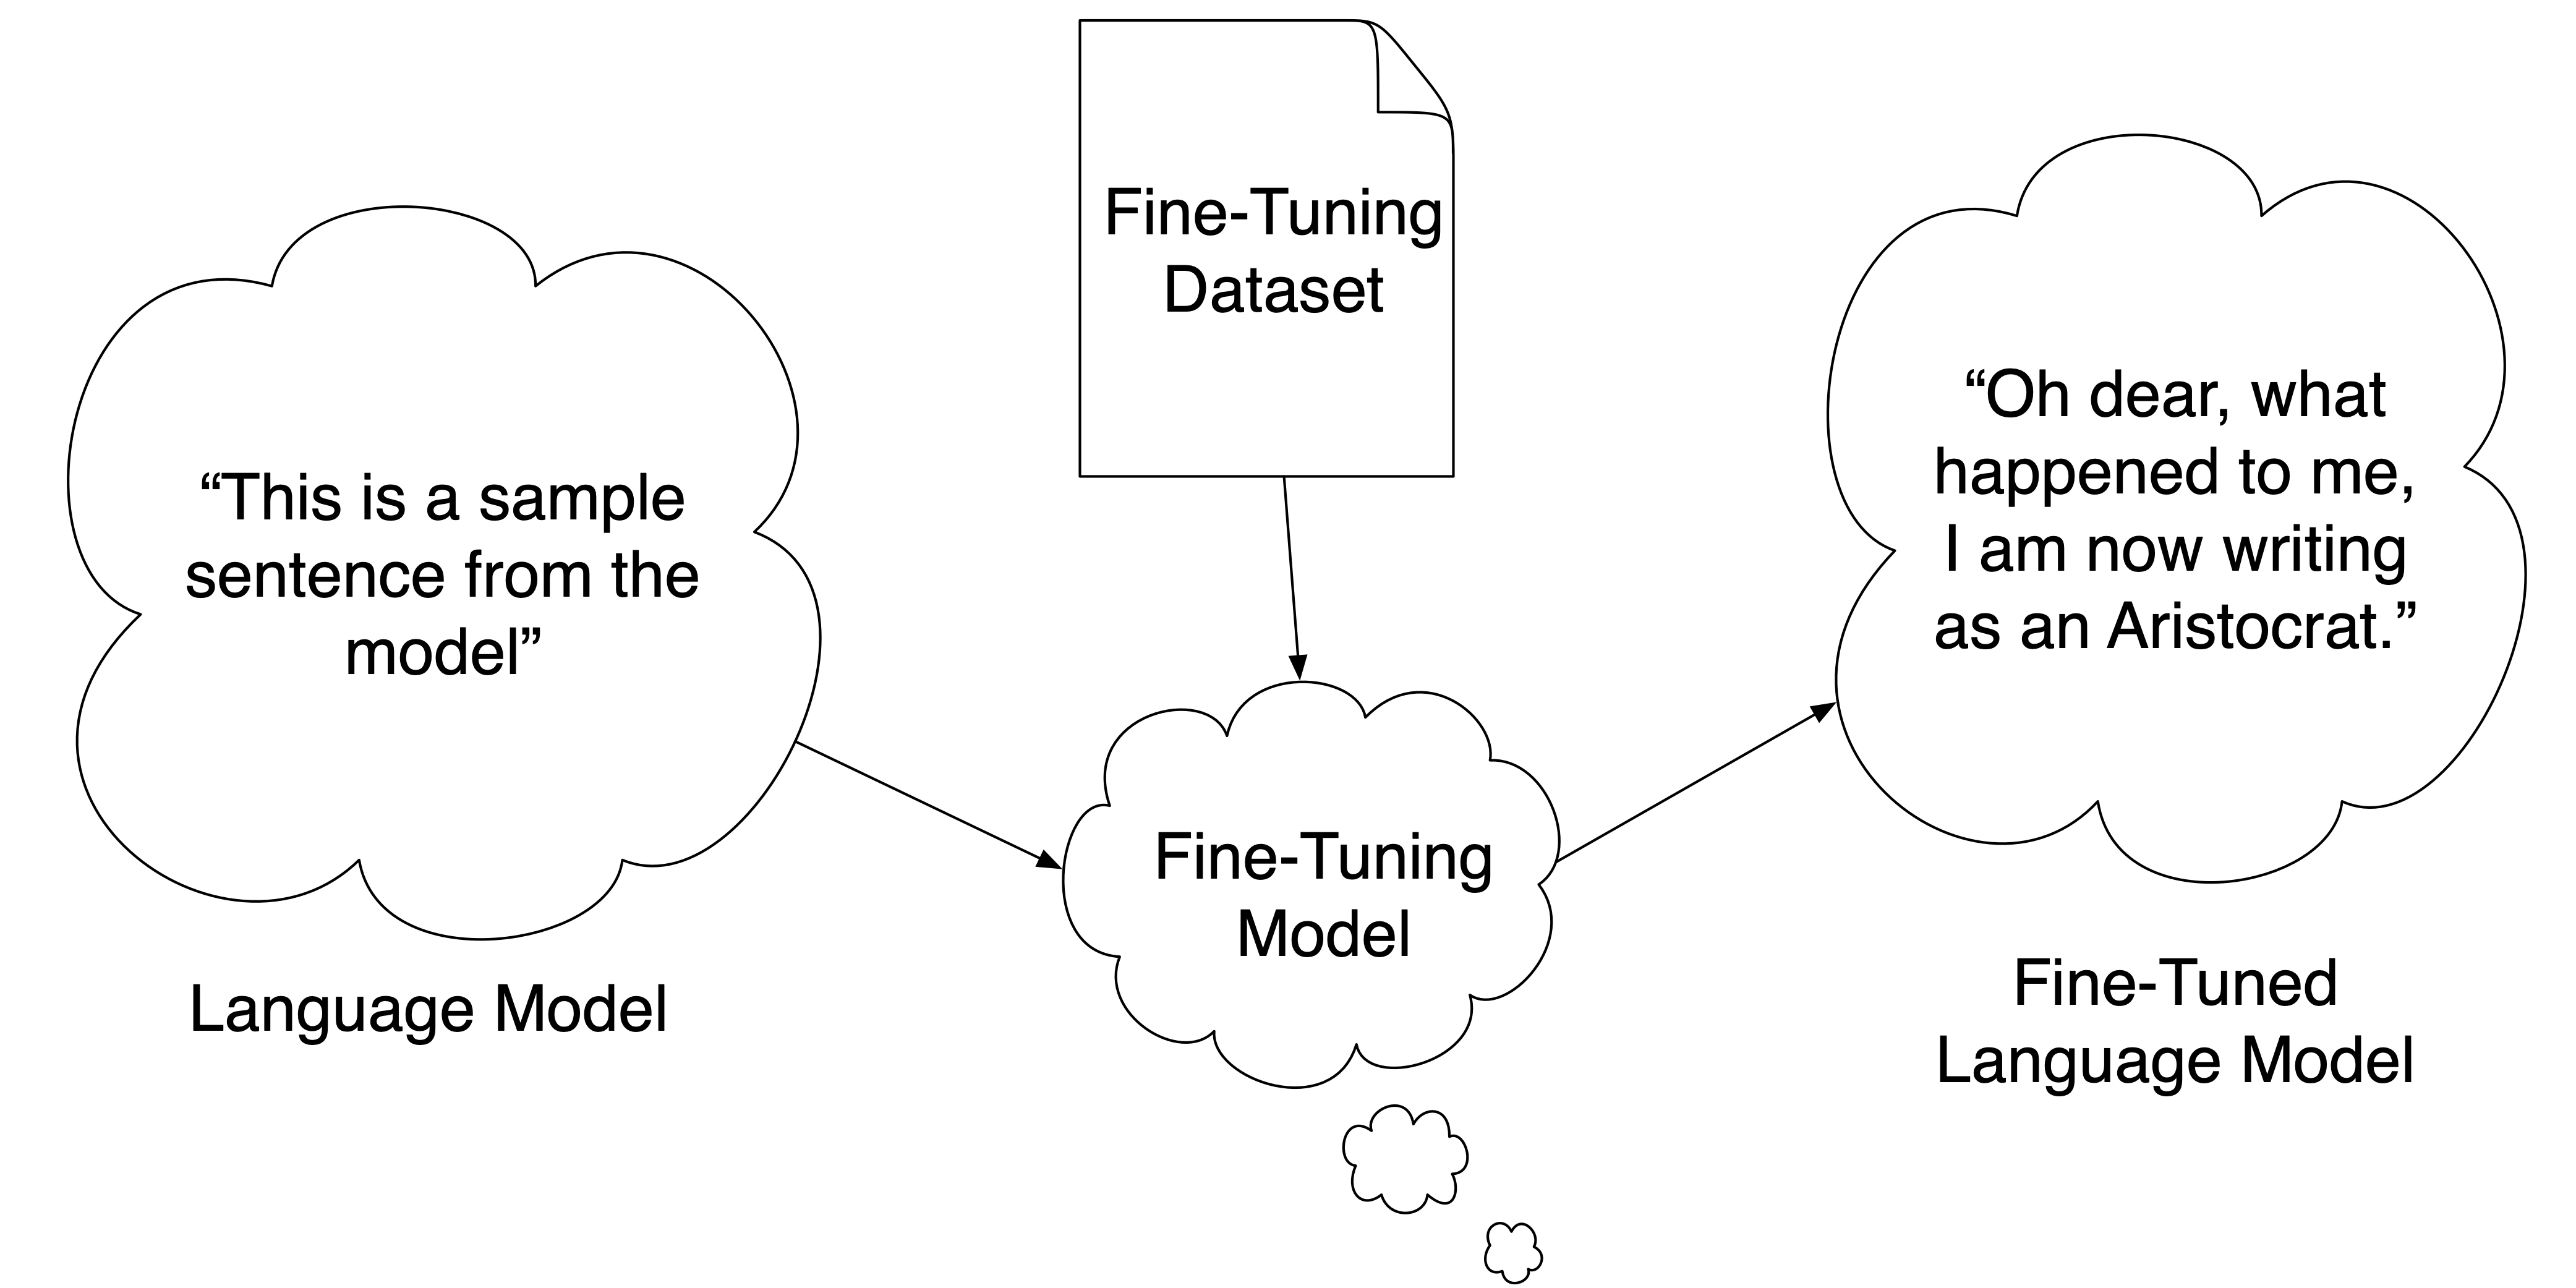
\includegraphics[width=\textwidth,keepaspectratio=true]{fig_finetunedmodel_chatbots}
    \caption{Illustrative representation of fine-tuning in a chatbot context.}
    \label{fig:fig_finetunedmodel_chatbots}
\end{figure}

\subsection{Reinforcement Learning}
\gls{rl} is proven to be very powerful by the latest research made by \textit{Open-AI} with its DOTA2 bot or \textit{Google's Deepmind} with AlphaZero, so we believe that it is worth mentioning it. However, this type of learning requires a finite state similar to a \gls{mdp}, which matches game cases but not conversations, and impacting by this means the motivation to export the technique to \gls{nlp}. Indeed, this methodology requires that all information required for the next step are wrapped into a single state to predict it, which makes it hard to use the dialogue case. For now, \gls{nlp} research does not provide a conclusion as, even with billions of simulations, \gls{rl} Chatbots could reach comparative results to Generative Chatbots \ref{chatbot:generative}.

\section{Grounded Chatbots}
\label{chatbot:grounded}
Falling in a particularly rare research field of \gls{ml} and \gls{nlp}, \gls{gl} can be seen as the future of \gls{mu} and \gls{mr}. In a chatbot context, the goal is to simulate, based on the Grounded Theory from the social sciences, how humans are using inductive reasoning to create conversations with unstructured knowledge. The idea is to give the ability to the bot, for any given input, to gather information from any data sources and provide an inductive output. E.g., Combining Knowledge Bases with weather forecaster. As a second example, for the given input: \say{What is the color in autumn of a leaf in Switzerland?}, 1) the bot would have first to identify the context keywords (color, leaf, autumn, switzerland), 2) the bot would select where to gather the information, 3) the would investigate the Wikidata Knowledge Base, Wikipedia, and The Weather Channel API, 4) the bot would formulate an answer based on the information it gathered. ~\ref{fig:fig_grounded_chatbots}

\begin{figure}
    \centering
    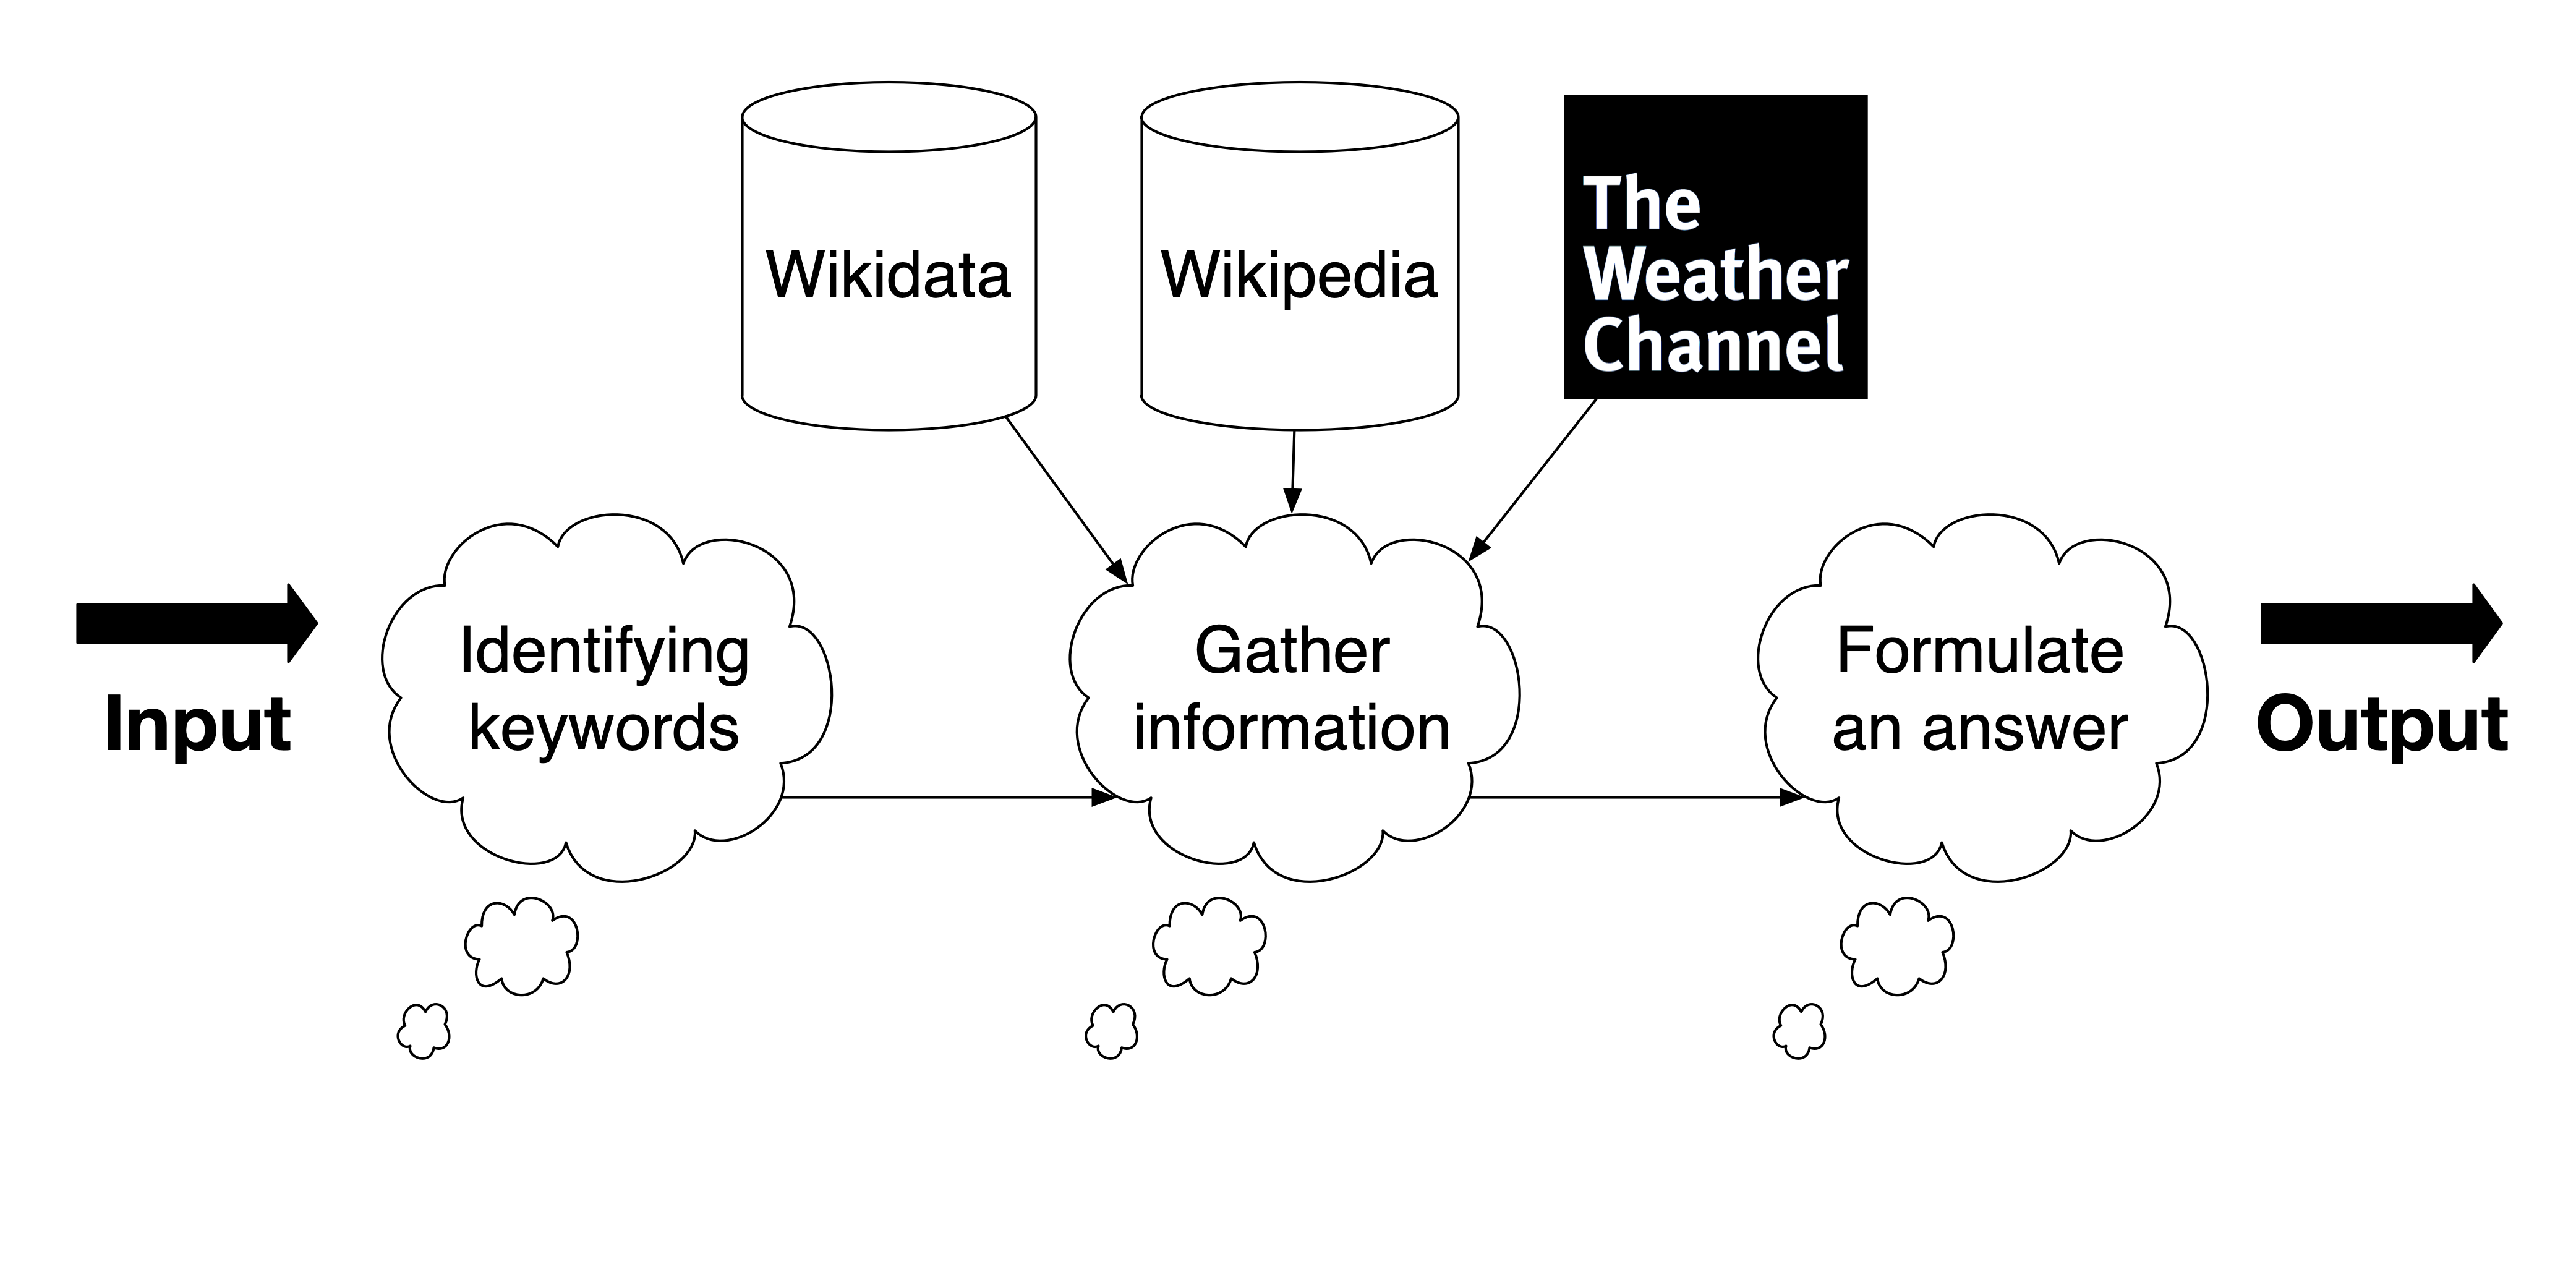
\includegraphics[width=\textwidth,keepaspectratio=true]{fig_grounded_chatbots}
    \caption{Illustrative representation of a grounded chatbot.}
    \label{fig:fig_grounded_chatbots}
\end{figure}

\section{Question-Answering Chatbots}
\label{chatbot:qa}
\gls{qa} is a prevalent task for chatbots; indeed, they are widely used for questioning tasks in either Single or \gls{open-domain}, Open or \gls{closed-ended}, Single or \gls{mh} with applications such as FAQs, Supports, help to find the meaning of life, and so on. Due to the broadness of the field, no defined methodology has been generalized; instead, it uses either one or multiple techniques described in the previous sections. It is interesting to note that the field of \gls{qa} is raising a lot of interest in \gls{nlp} research lately, and the benchmarking game of creating the new baselines, with increasingly complex datasets, is still in progress. In this section, we will overview some recent baselines.

\paragraph{Fine-Tunning Language Models} Large \gls{lm} such as BERT \autocite{paper:devlin-etal-2019-bert} or GPT-2 \autocite{papers:gpt2} are often fine-tuned on \gls{qa} datasets similar to SQUAD 2.0 \autocite{paper:rajpurkar-etal-2018-know} which are particularly tricky, even for humans.

\label{chatbot:templates}
\paragraph{Querying Models} Based on \gls{qa} datasets, a model is trained to fill structured templates.  The generated output is a structured query for a particular querying language such as SPARQL for Wikidata. 

\paragraph{Retrieval} A popular approach in the industry is to use tools such as Elasticsearch for indexing and additional tools using \gls{ml} heuristics to perform the queries.

\clearpage
\section{Common Chatbot Features Overview}
In this section, we are non-exhaustively naming a few recurring features appearing during our targeted research.

\subsection{Context}
Humans are intuitively and extensively relying on the context for conversational purposes, which implies similar capacities from dialogue-based chatbots. On a side note, one-way style dialogues such as commands or none-nested questions do not need to hold context to perform well.

\paragraph{Short term context} Implying the ability for the bot to hold context for at least the current conversation, e.g., few keywords or on-the-fly \gls{model-ft}.

\paragraph{Long term context} Often, chatbots would use user-profiles as part of their architecture to remember information such as the favorite pizza flavor of a client. 

\subsection{Proactivity}
Simulating personalized interest as a human would do is not new to chatbots, as it has been proven by becoming a standard in marketing and customer support chatbots. Messages such as \say{Hey, you have been on our web store for a while, can I help you?}, are carrying a sense of proactivity; however, beyond asking general pre-made questions, limitations are clear, and not much progress has been made yet in the field. Indeed, human-like proactive chatbots imply algorithms capable of initiating conversations by initiating a dialogue or asking information in a meaningful manner based on the long and short term context.

\subsection{Narrow vs General Chatbots Scope}
Beyond the three main categories \ref{chatbot:main-cats} identified during the study, in general, chatbots can additionally be classified within a scope starting at Narrow Chatbots up to General Chatbots. To position them, we defined a two axes classification using Tasks and Knowledge as represented on Table \ref{tab:agi-ani}.

\paragraph{Tasks Axis}
To name a few examples of task-oriented Chatbots: Talk, \gls{faq}, Customer Support, or Ordering.

\paragraph{Knowledge Axis}
Non-exhaustively, as follows, a few knowledge-centric examples for chatbots: Health, Weather, or Customer Service.

\paragraph{Narrow Chatbots}
Narrow chatbots are limited by the range of tasks they can accomplish and the knowledge they can use. By design, they are very good at a particular task for a particular knowledge requirement.

\paragraph{General Chatbots}
They are neither limited by the range of tasks they can accomplish nor by the knowledge they can use. However, they often have an average performance for any task or knowledge. We go in more details at section \ref{chatbot:general}.


\newcommand\MyBox[2]{
  \fbox{\lower0.75cm
    \vbox to 2cm{\vfil
      \hbox to 6cm{\hfil\parbox{5cm}{#1\\#2}\hfil}
      \vfil}
  }
}

\setlength\tabcolsep{0pt}
\begin{table}
\centering
\begin{tabular}{c >{\bfseries}r @{\hspace{0.7em}}c @{\hspace{0.4em}}c @{\hspace{0.7em}}l}
  \multirow{6}{*}{\rotatebox{90}{\parbox{2.4em}{\bfseries\centering Tasks}}} 
  & & \MyBox{Expert in a specific Field}{Expert at all Tasks} & \MyBox{\textbf{General Chatbots}\\Expert in all Fields}{Expert at all Tasks} \\[2.4em]
  & & \MyBox{\textbf{Narrow Chatbots}\\Expert in a specific Field}{Expert at specific Task} & \MyBox{Expert in all Fields}{Expert at specific Task} \\[2.4em]
  & & \multicolumn{2}{c}{\bfseries Knowledge} & \\
\end{tabular}
\caption{This table represents categories in Narrow and General Chatbots in a Tasks versus Knowledge format.}
\label{tab:agi-ani}
\end{table}


\subsection{General Chatbots}
\label{chatbot:general}
As research progresses in the \gls{nlp} field, chatbots are improving as an effort to perform simultaneously well in various tasks and multi-knowledge bases. As a contemporary goal, in addition to any chatbot related tasks and broad knowledge expertise, General Chatbots must not be limited to their current capabilities, but on the contrary, be able to learn new tasks and subjects continuously. As far as we as this study went, we could not find \gls{sota} general chatbots as defined. However, companies like \textit{Amazon} are selling to a large public a feel to general chatbots with Alexa. Indeed, apart from ordering goodies from \textit{Amazon} and roughly conversing with Alexa, users can command their smart homes, use it as a personal assistant, or even program \textit{skills} to perform custom actions.

\clearpage
\section{Chatbots Cartography}
As a result of this chapter, we created a chart on Figure ~\ref{fig:fig_chatbot_cartography} representing the current state of chatbots from our point of view. Note that a particular use-case could be in multiple leafs.

\begin{figure}
    \centering
    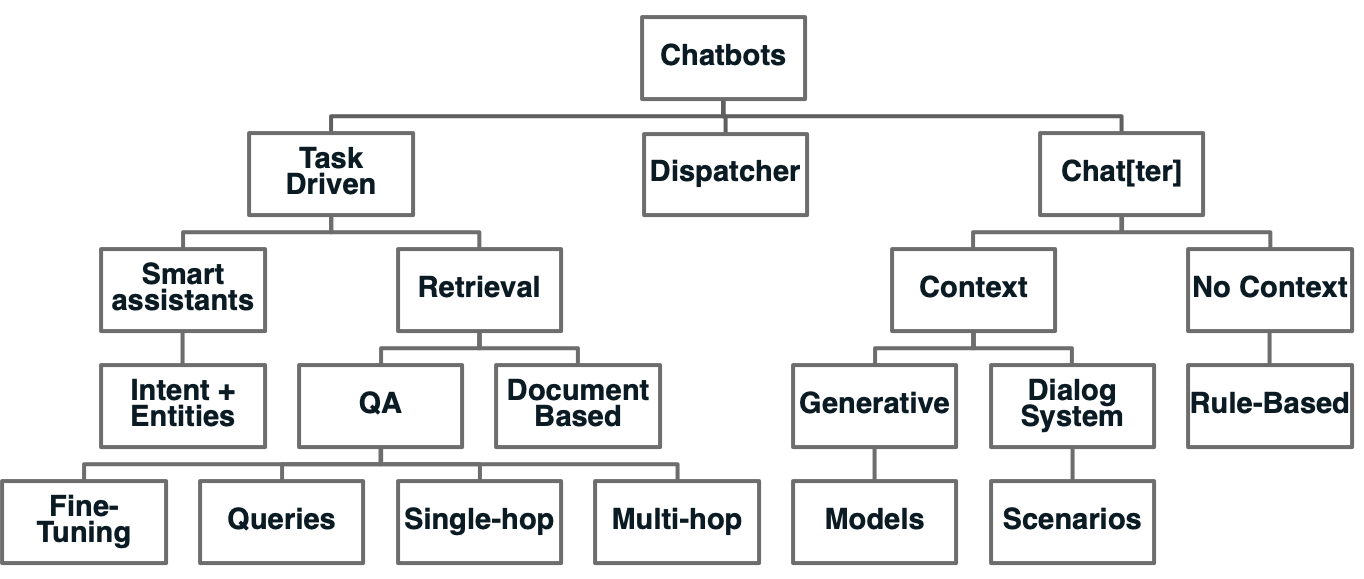
\includegraphics[width=\textwidth,keepaspectratio=true]{fig_chatbot_cartography}
    \caption{Represents the chatbots cartography as conclusion to the chatbot state-of-the-art chapter.}
    \label{fig:fig_chatbot_cartography}
\end{figure}






\chapter{Natural Language Processing}
\label{chap:nlp}

It is often challenging to realize the complexity behind \glsfirst{nl}, even to experts. First of all, Language is an academic field of study, implying multi-disciplinary skills. And secondly, staying up to date with evergrowing tools and new \gls{sota} algorithms proves to be challenging. \gls{nl} is the fundamental communication element for humans, \gls{nlp} is the field of \gls{ml} studying \gls{nl} with the goal of providing the ability to machines to handle and mimic \gls{nl} to create human-like verbal interactions. Beyond words and grammar rules, \gls{nl} is a complex orchestration of subtleties, intuitively handled by humans, but not easily handled by machines. Nonetheless, \glspl{nlp} technologies are massively used in our daily lives, including information extraction, summarization, and conversation simulation. However, even if machines are given the same language rules as humans, they do not yet understand the manipulation they are processing, as humans would do. Indeed, \gls{nlp} algorithms are applying pre-defined or multiple examples-based learned rules, which may result in ambiguities while applying \gls{nl}. Using a rule-based approach (as seen in Chapter \ref{chatbot:rulebased}) to build a \gls{nl} model would result into near to infinite amount of conditions, this is the main reason for \gls{nlp} to be particularly present \gls{ml}, particularly in \gls{dl}. 


%\section{\acrlong{nlp} Technologies}
\section{Word Embeddings}
\label{nlp:we}
The technique is commonly used as the first data pre-processing for \gls{dl} in \gls{nlp} tasks. Those \glsfirst{ul} algorithms capture syntactical and semantical words representation from large unlabelled corpora datasets as vectors by building a multi-dimensional matrix. On average, dimensions are held in a scope of 100 to 400, and thanks to the vectorized nature of captured words, geometrical operations can be applied, such as the cosine functions to calculate word similarities. Another feature related to word embeddings is the ability to apply analogical operations such as \textit{'king' - 'man' + 'woman' = 'queen'}, which popularize Word2Vec \ref{nlp:word2vec} and gave credits to the method, even if the justification to this effect has been theorietized 4 years later \footnote{Skip-Gram - Zipf + Uniform = Vector Additivity \autocite{paper:gittens-etal-2017-skip}} by stating that the compositionality is only seen when assumptions are held, in particular when words are uniformly distributed in the embedding space.

\subsection{Word2Vec and GloVe}
\label{nlp:word2vec}
Published by \textit{Google} in 2013, Word2Vec \autocite{paper:word2vec}, and its competitor GloVe \autocite{paper:glove} published by the \textit{University of Standford} in 2014, both use a \gls{snn}, as illustrated on Figure ~\ref{fig:fig_snn}, similarly to \gls{sl} by feeding as input a text corpora, and outputting word vectors with a given vocabulary. Training and testing is straightforward but painful tweaking makes it hard to build good generalized word embedding representations. Even if the \gls{snn} could remind a \gls{dl} approach, it is only has one hidden layer; however, the output word vectors are particularly useful for \gls{dnn} as input.

\begin{figure}
    \centering
    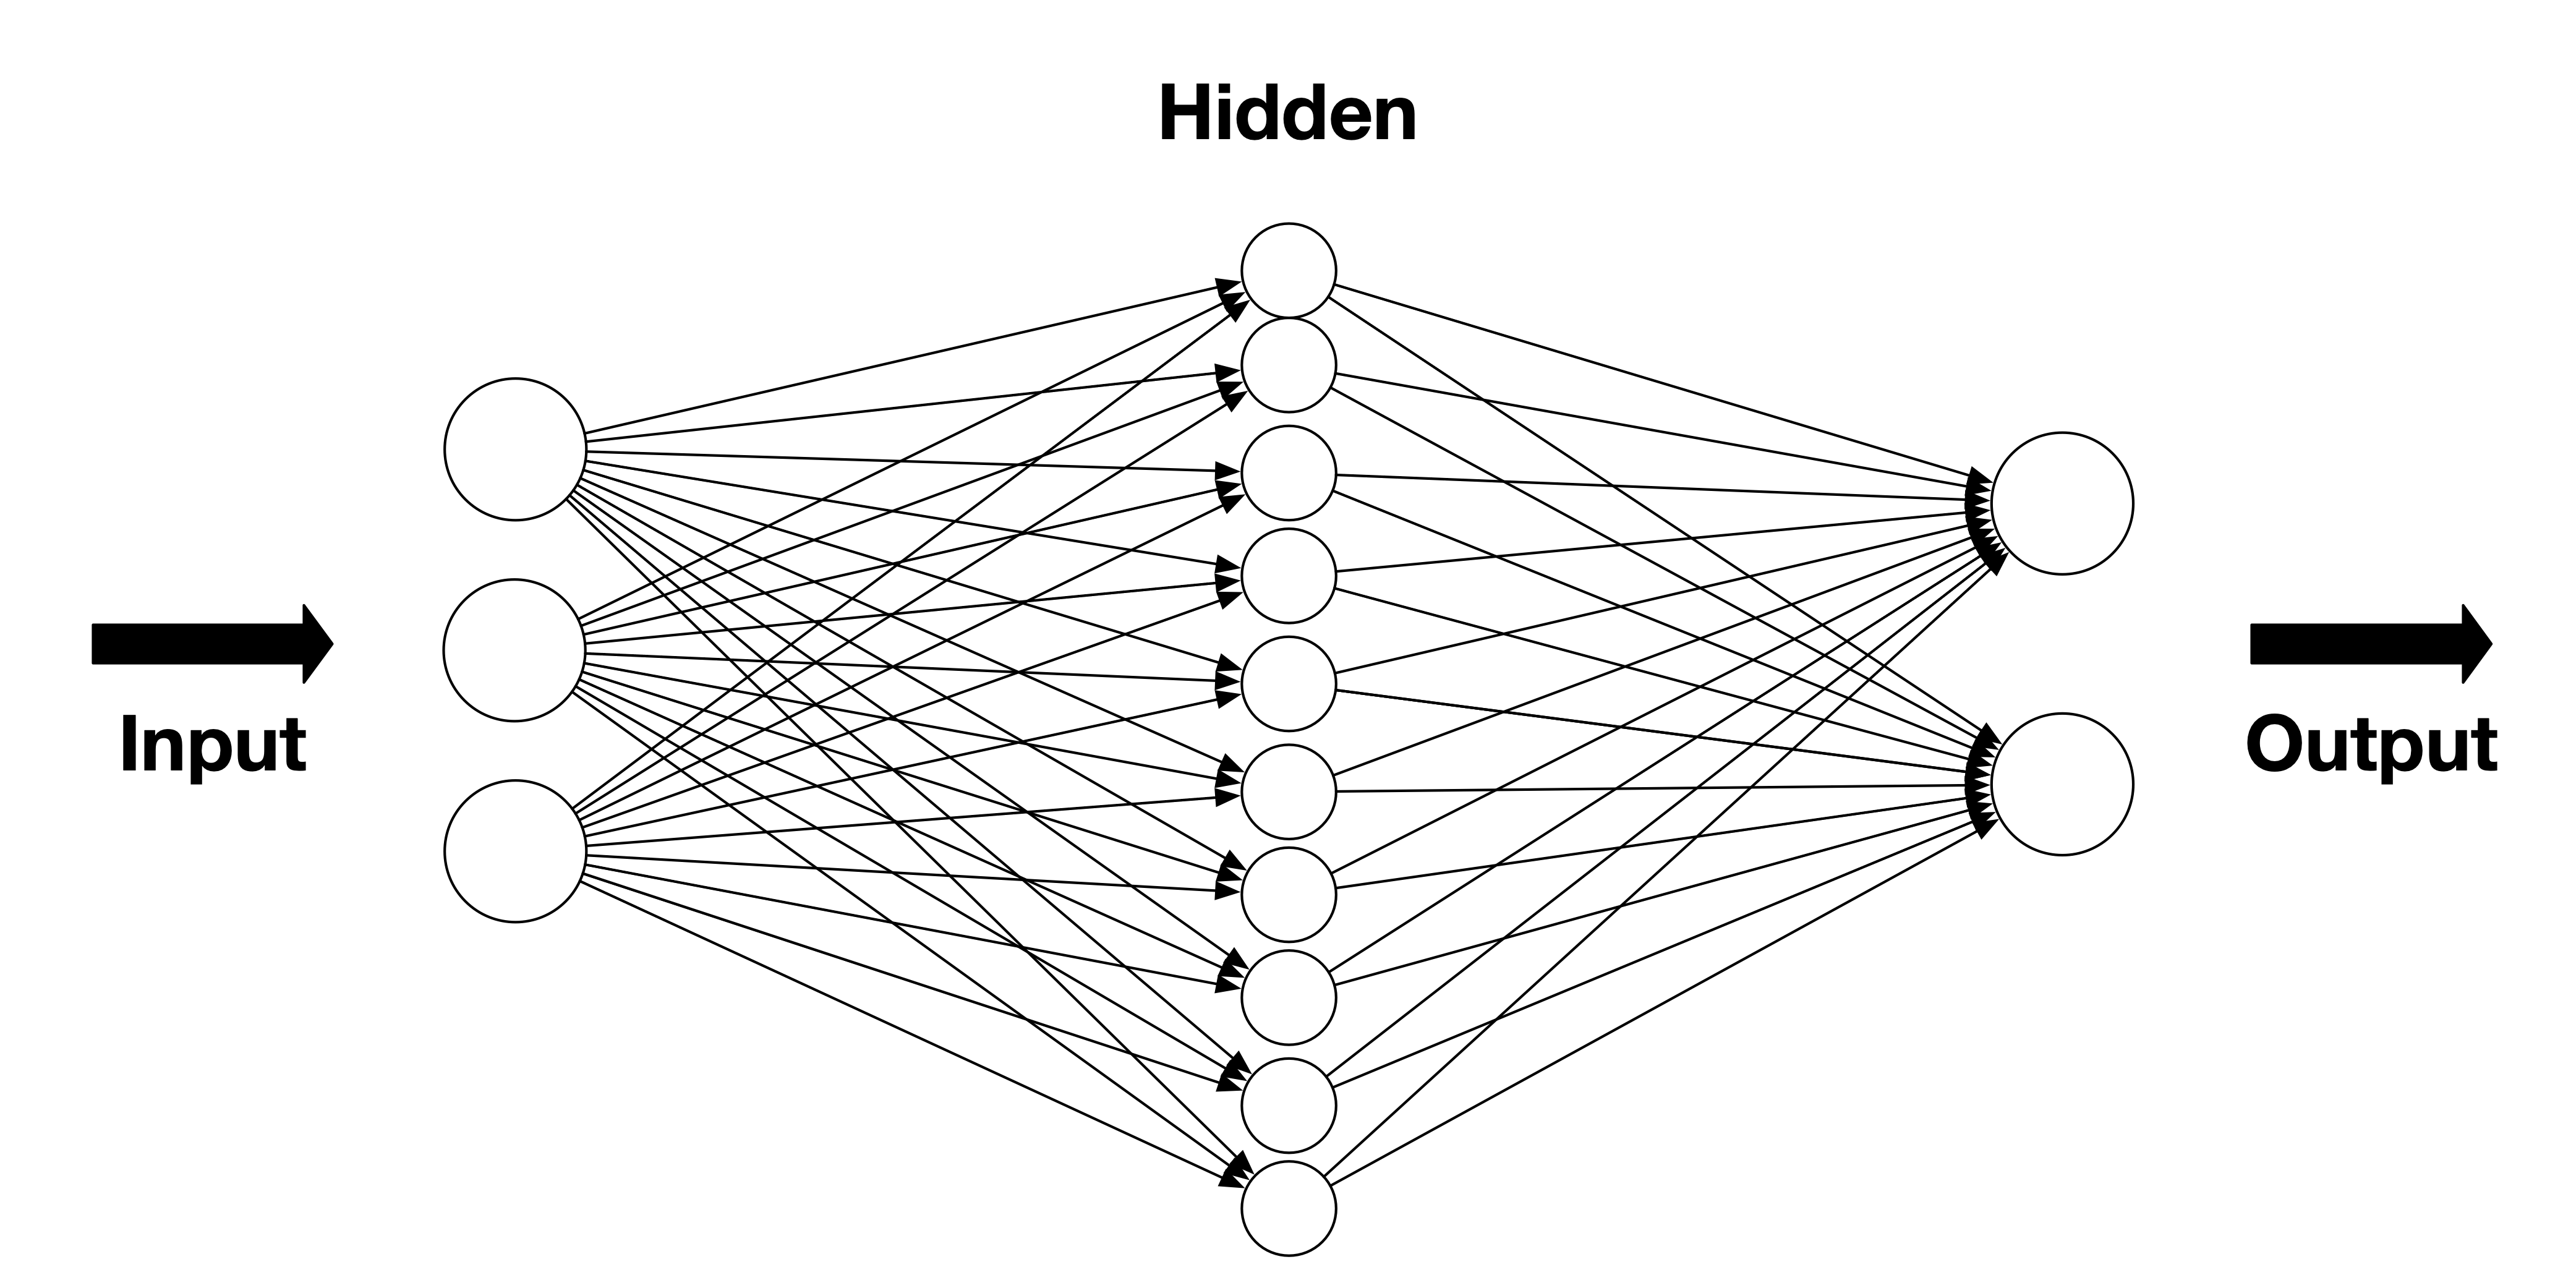
\includegraphics[width=\textwidth,keepaspectratio=true]{fig_snn}
    \caption{Illustrative representation of a Shallow Neural Network}
    \label{fig:fig_snn}
\end{figure}

\subsection{Out of Vocabulary Problem}
\label{nlp:oov}
A common issue in \gls{we} is related to the vocabulary itself when words are unknown, called the \gls{oov} issue. The issue occurs when post-training the model is requested to provide a vector representation that it has never seen before. A solution could be to handle the exception by forwarding it to a default or pre-defined error vectors such as a series of zeros. We could approach the problem sophisticatedly, by defining on-the-fly \gls{oov} words with at a high learning rate as the sum of word-vectors contextualizing the \gls{oov}  \autocite{paper:journals/corr/HerbelotB17}. Another solution would be to fallback to \ref{nlp:ce} by either training a model to compositional map characters to words \autocite{paper:journals/corr/PinterGE17}, or using \gls{ce} as a whole instead of \gls{we} \ref{nlp:ce}.

\section{Character Embeddings}
\label{nlp:ce}
Additionally to \gls{we} similar abilities to capture semantics and syntactic relations, \gls{ce} handles by design \gls{oov} issues \ref{nlp:oov}, which is common for rich vocabularies languages. Instead of using words as vocabulary, \gls{ce} uses individual characters and semantics embeds words using the characters compositionally, which avoids word segmentation and makes it useful for language such as Chinese \autocite{paper:conf/ijcai/ChenXLSL15}. Moreover, \gls{ce} can also perform complementary \gls{nlp} tasks such as \gls{pos-tag} \autocite{paper:conf/icml/SantosZ14}, \gls{ner} \autocite{paper:ma-etal-2016-label}, Sentiment Analysis \autocite{paper:2017HaoYetal} and \gls{lm} \autocite{paper:journals/corr/KimJSR15}. As it is at the time of writing, \textit{FastText} based on the a morphologically-rich skip-gram approach \autocite{paper:journals/corr/BojanowskiGJM16} has been popularilized due to its ability to be scalabely trained on large corpora fast, and effectively. 

\section{Language Models}
\label{nlp-lm}
Beyond complex semantics and syntaxes provided by \gls{we} \ref{nlp:we} and \gls{ce} \ref{nlp:ce}, \glspl{lm} handles \gls{cwe} by additionally capturing the polysemy across multiple contexts. Indeed, it was discovered that a distributed semantic, such as \gls{we} and \gls{ce} are not sufficient to infer context within the embeddings \autocite{paper:journals/corr/LucyG17}. A solution is to combine overall word representations from \gls{we} with \textit{ELMo} \autocite{paper:journals/corr/abs-1802-05365}, as its authors suggest, a \gls{bilm} able to build deep contextual word embeddings by handling multiple word representations. As mentioned in the study, handling polymesy is just one of the \glspl{lm} features as they are theoritized to capture meaningful \gls{nl} traits used in \gls{nlu} and \gls{nlg}. To increase the \gls{lm} quality, defined by language syntactic and semantical complexities captured, \gls{ul} on large corpora is popularly used, as no labeled data is required.


\section{Transformers}
\label{nlp:transformers}
The year 2017 has set a milestone in \gls{nlp}, transformers \autocite{paper:journals/corr/VaswaniSPUJGKP17} are since then defining the \gls{sota} for multiple \gls{nlp} tasks mainly due to its parallelized attention \ref{nlp:attention} architecture. Large multi-directional pre-trained \gls{lm} such as \gls{gpt2} or the \gls{bert} family are, additionally to their ability to capture features at sentence level, out-performing by a large margin previously mentioned \gls{nlp} technics at tasks such as \gls{qa} by performing \gls{model-ft}, an adaptation of the very popular Transfer Learning feature from computer vision. Making those new \gls{lm} currently trendy among \gls{nlp} researchers and engineers.

\begin{figure}
    \centering
    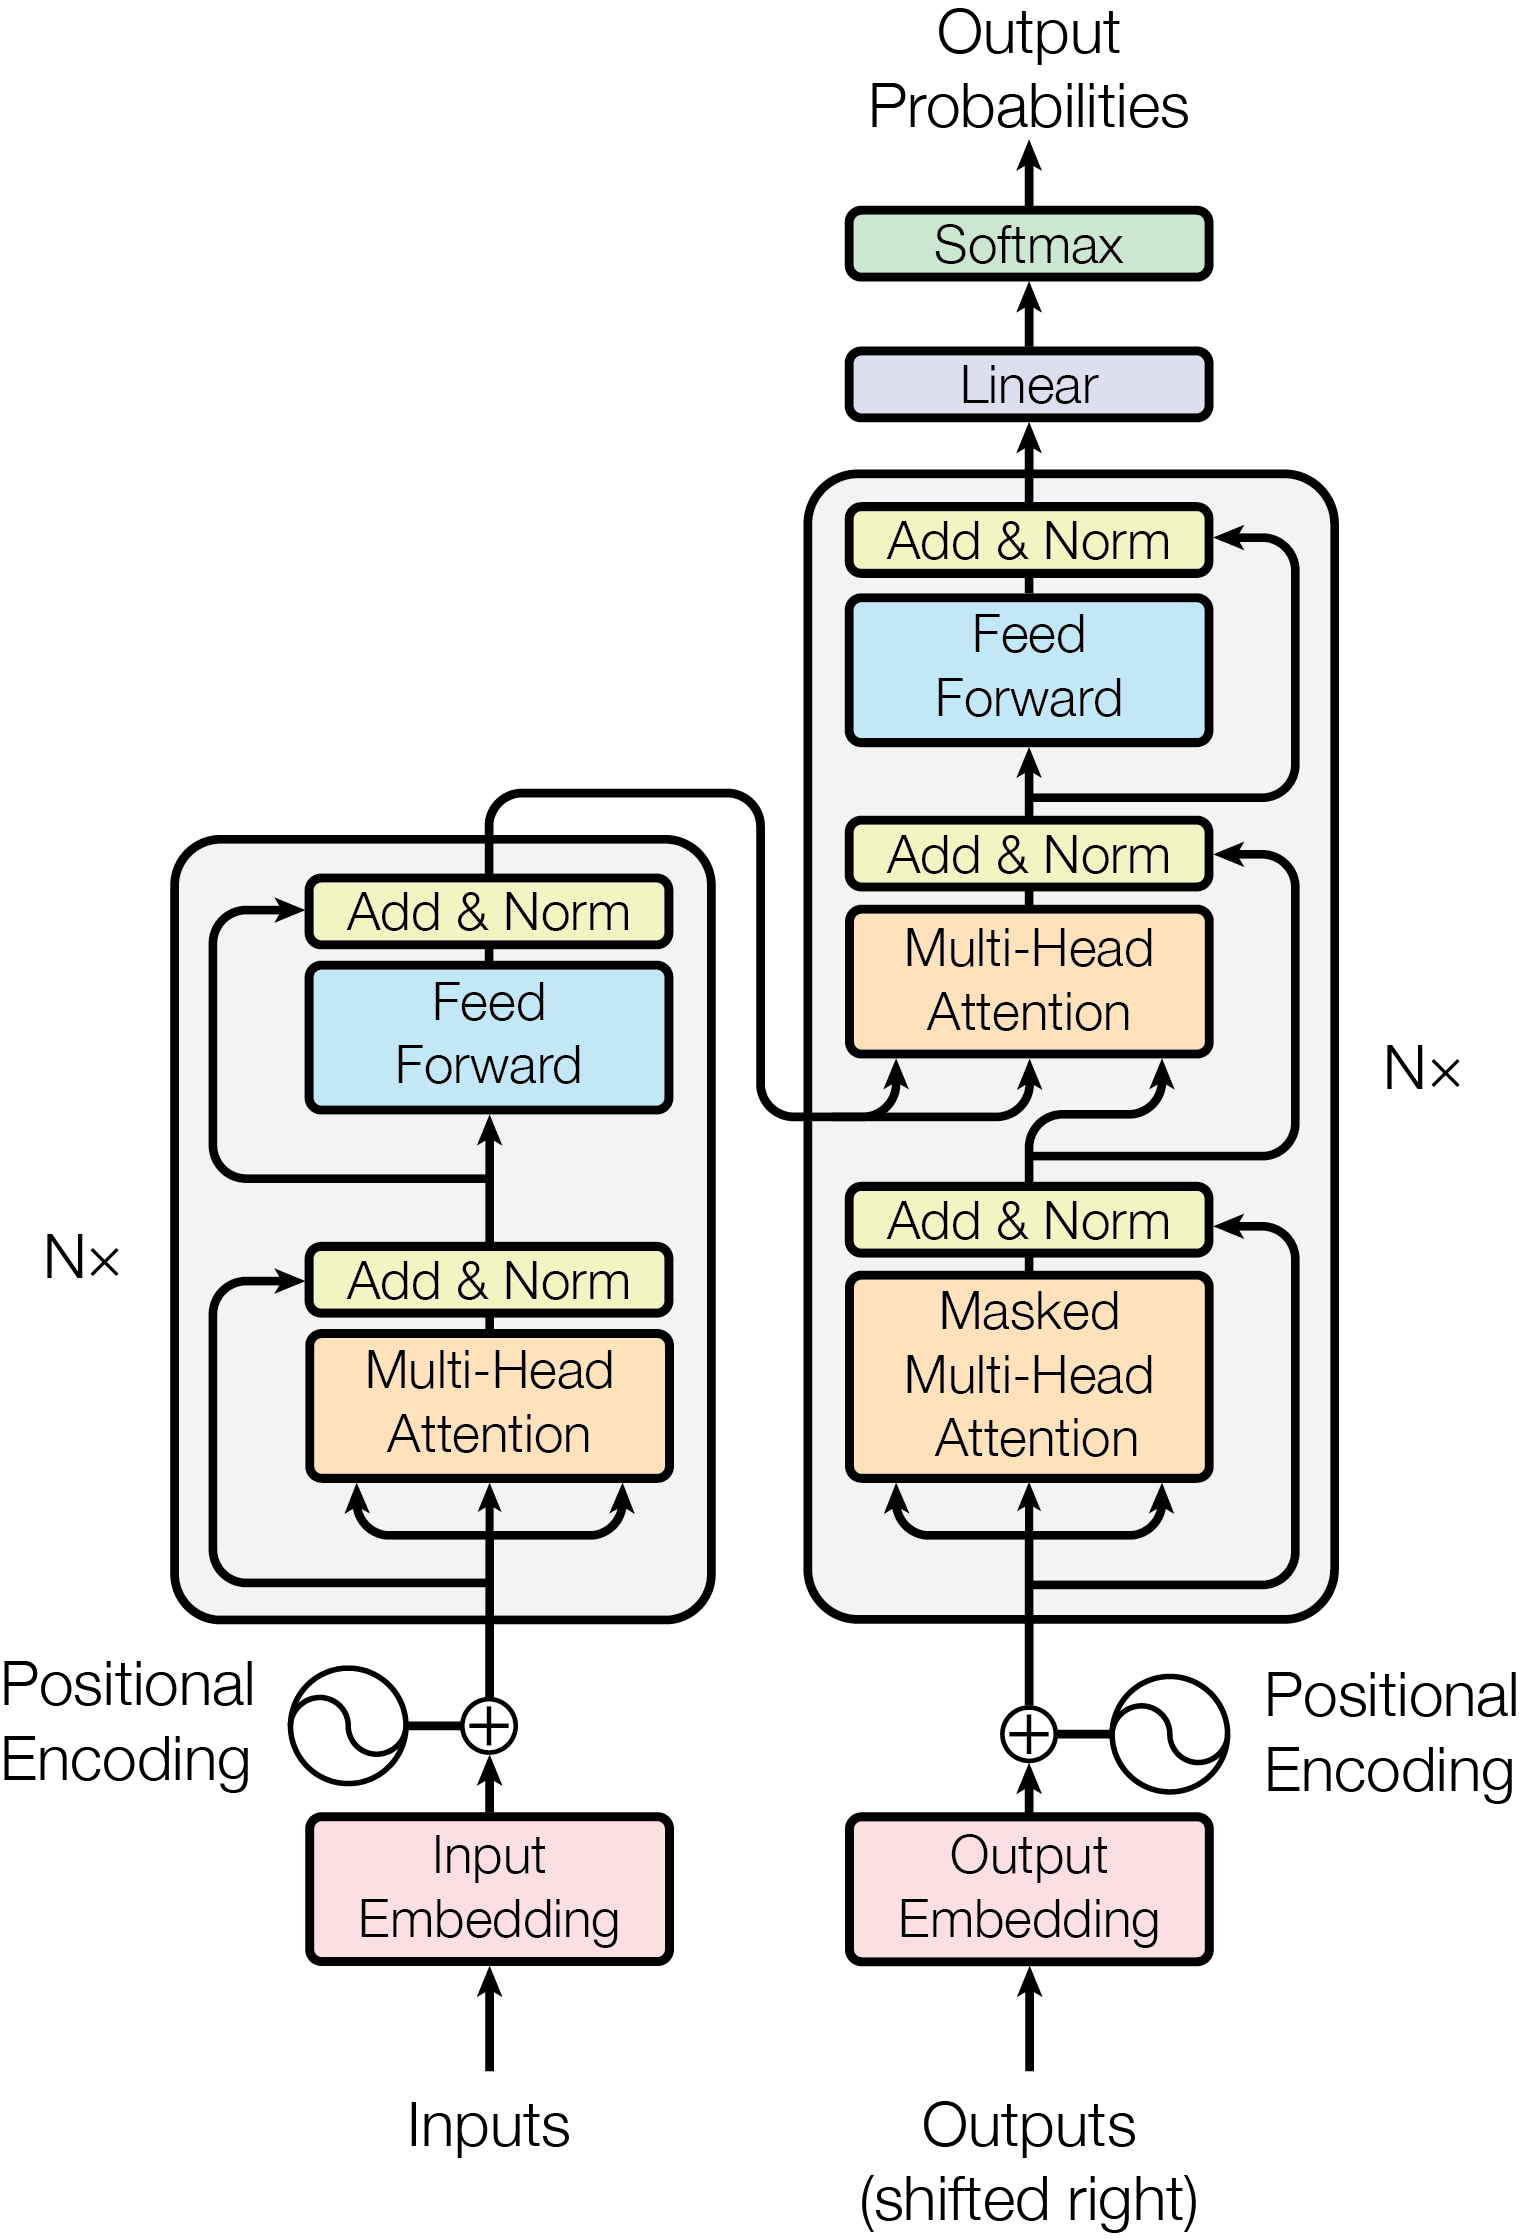
\includegraphics[width=\textwidth/2,keepaspectratio=true]{fig_external_transformer_1}
    \caption{Represents the Transformer architecture. Figure 1 from \autocite{paper:journals/corr/VaswaniSPUJGKP17}}
    \label{fig:fig_external_transformer_1}
\end{figure}

\subsection{Attention Mechanism}
\label{nlp:attention}
Introduced in 2014, The Attention Mechanism \autocite{paper:bahdanau2014neural} solved the problem raised by tasks such as text summarization, machine translation, or sentiment analysis, where the input is often too rich to perform a selective encoding. Originally, the last hidden state of the decoder is used by a multi-layer perceptron to define the attention from an input hidden state. The mechanism even got adapted from \gls{nlp} to Computer Vision and shown its ability to replace \gls{cnn} with \gls{sota} results \autocite{paper:journals/corr/abs-1906-05909}.

\begin{figure}
    \centering
    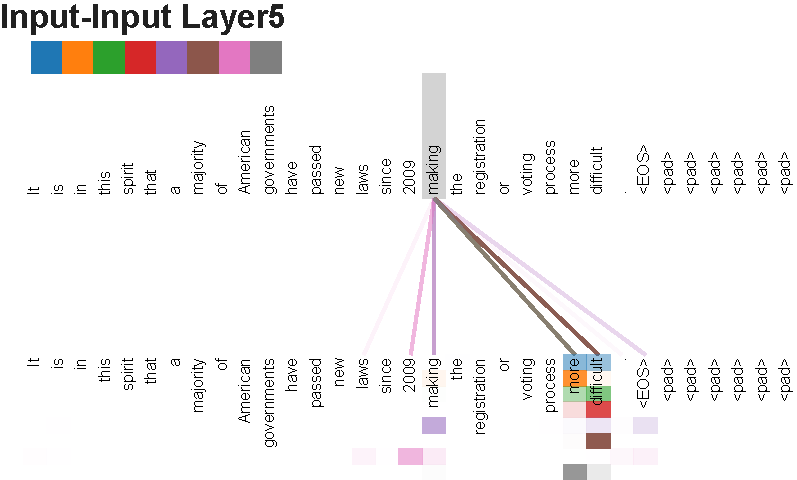
\includegraphics[width=\textwidth,keepaspectratio=true]{fig_external_transformer_3}
    \caption{Illustrates the attention mechanism for long-distance dependencies handled via multiple attention heads used in transformers. Figure 3 from \autocite{paper:journals/corr/VaswaniSPUJGKP17}}
    \label{fig:fig_external_transformer_3}
\end{figure}

\subsection{The architecture}
Even if Transformers, Figure \ref{fig:fig_external_transformer_1}, are using a \gls{seq2seq} approach similar to \gls{enc-dec}, which reminds of \gls{rnn} and \gls{cnn}, the overall architecture focuses on the attention mechanism to capture the relation between the input and the output, making it well parallelizable and less time consuming during training with its multi-attention heads approach. Multi-heads, Figure \ref{fig:fig_external_transformer_2_1}, uses sets of queries Q, keys K and values V to perform attention with dot-products, Figure \ref{fig:fig_external_transformer_2_2}. In other words, the multi-head attention mechanism builds a multi-dimensional matrix representing each word vectors the attention relatives to all word vectors in a predefined window, such as a sentence, then computes the overall attention for each word vectors. In addition to the attention centric mechanism, transformers are also using proven \gls{dl} techniques such as layer normalization, dropouts, and positional encodings.

\begin{figure}
	%\hfill
	%\centering
	\begin{subfigure}{.5\textwidth}
		\centering
		%
\includegraphics[width=.4\linewidth]{image1}
		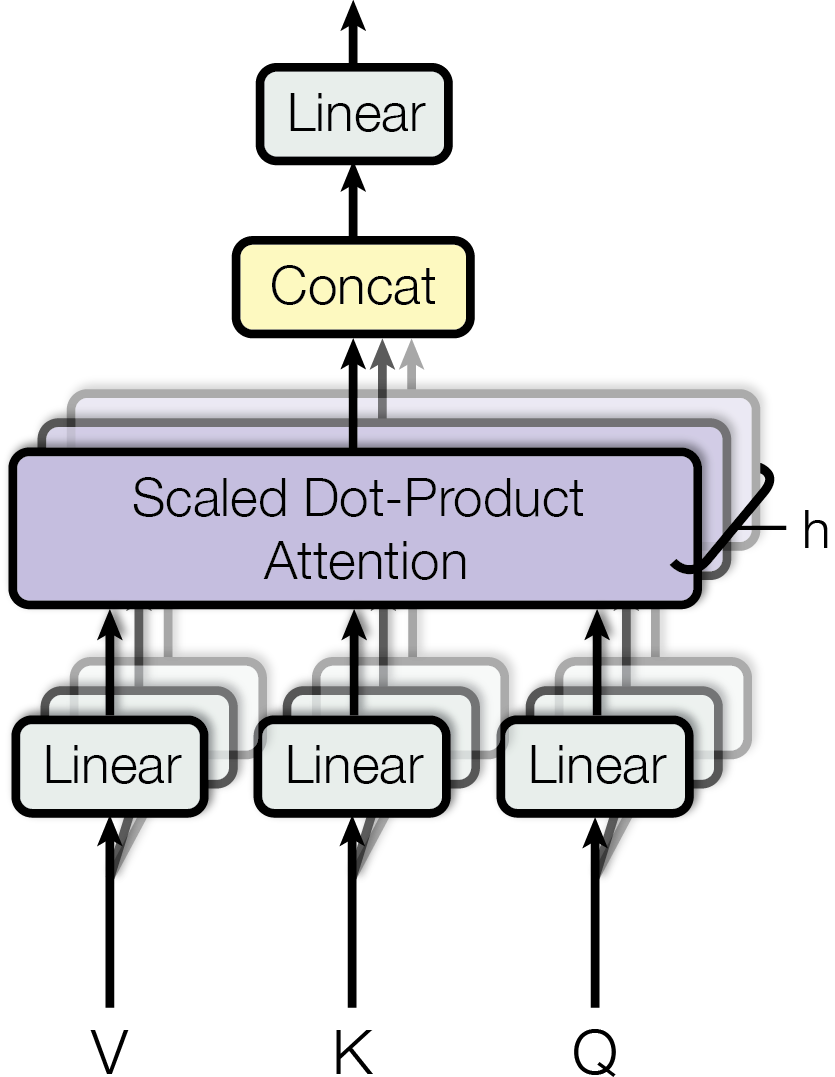
\includegraphics[width=\linewidth, height=1.2\linewidth, keepaspectratio=true]{fig_external_transformer_2_1}
		\caption{Multi-Head Attention mechanism.}
		\label{fig:fig_external_transformer_2_1}
	\end{subfigure}
	\hfill
	\begin{subfigure}{.5\textwidth}
		\centering
		%
\includegraphics[width=.4\linewidth]{image1}
		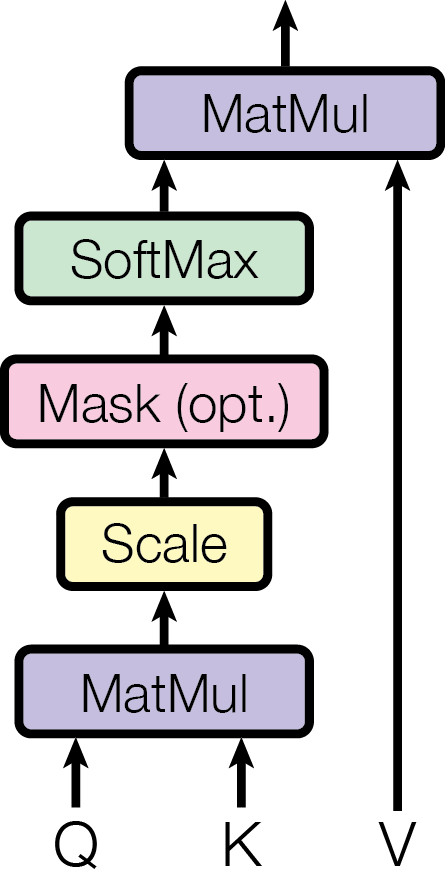
\includegraphics[width=1\linewidth, height=1.2\linewidth, keepaspectratio=true]{fig_external_transformer_2_2}
    	\caption{Scaled Dot-Product Attention used by the Multi-Heads Attention \ref{fig:fig_external_transformer_2_1}}
    	\label{fig:fig_external_transformer_2_2}
	\end{subfigure}
	%\hfill
	\caption{Multi-head attention anatomy extracted from Figure 2 of \textit{Attention is All you Need} \autocite{paper:journals/corr/VaswaniSPUJGKP17}}
	\label{fig:fig_external_transformer_2}
\end{figure}


\section{Honorable Mentions}
Even if Transformers have deprecated \gls{cnn} and \gls{rnn} in \gls{nlp} by solving their main bottleneck implying the sequential processing during encoding with the Attention Mechanism \ref{nlp:attention}. We still wanted to mention them as those techniques have defined baselines at multiple \gls{nlp} tasks for many years.

\subsection{Convolutional Neural Networks}
Commonly used in sentence modeling thanks to their good ability at mining semantics; however, their models are relatively heavy for the task performed. Additionally, they do not perform well on large windows, resulting in bad context handling for long-distance spread information and order tracking. In the field of \gls{qa}, interesting approach as been researched, such as Multi-Column \gls{cnn} \autocite{paper:Dong2015} able to treat multiple aspects of questions by building compatible representations with Wikidata's ancestor \textit{Freebase} \autocite{paper:bollacker2008}. In 2016, one of the final promising \gls{cnn} approach was introduced for \gls{qa} with a model able to handle relational information by word matching question and answer pairs \autocite{paper:Severyn2016}.

\subsection{Recurrent Neural Networks}
 By design and compared to \gls{cnn}, \glspl{rnn} try to take advantage of their ability to remember previous computations. However, it appears that no clear performance winner at \gls{nlp} tasks demarks \gls{rnn} from \gls{cnn} \autocite{paper:Yin2017}; indeed, their parallel performances depends on the global semantics and the task itself. Similarly to \gls{cnn}, \gls{rnn} is broadly used for \gls{nlp} tasks such as Language Modeling, Machine Translation, and Word/Sentence Classification.

\subsection{Memory Networks}
Also named MemNet \autocite{paper:Weston2015MemoryN}, the technique is still actively researched in the field of \gls{nlp} as it provides an intuitive approach to attention by using \gls{mh} \autocite{paper:journals/corr/TangQL16}, and sets the technique as an interesting competitor to Transformers \ref{nlp:transformers}. As the \gls{attention} \ref{nlp:attention} builds sets of hidden vectors with its encoder, \glspl{mn} uses the hidden vectors as internal memory instead of feeding them to a decoder for token generation. Further in the \glspl{transformer} competition, \glspl{mn} can be applied to similar \gls{nlp} tasks such as \gls{qa} \autocite{paper:journals/corr/KumarISBEPOGS15} by extending the \textit{(Representation, Attention, Answer)} tuples to \textit{(Memory, Question, Answer)} tuples. The Figure \ref{fig:fig_external_memnet} presents a \gls{qa} Memory Networks based architecture using knowledge base as knowledge source as initial Key-Value Memories provider, \glspl{spo}.

\begin{figure}
    \centering
    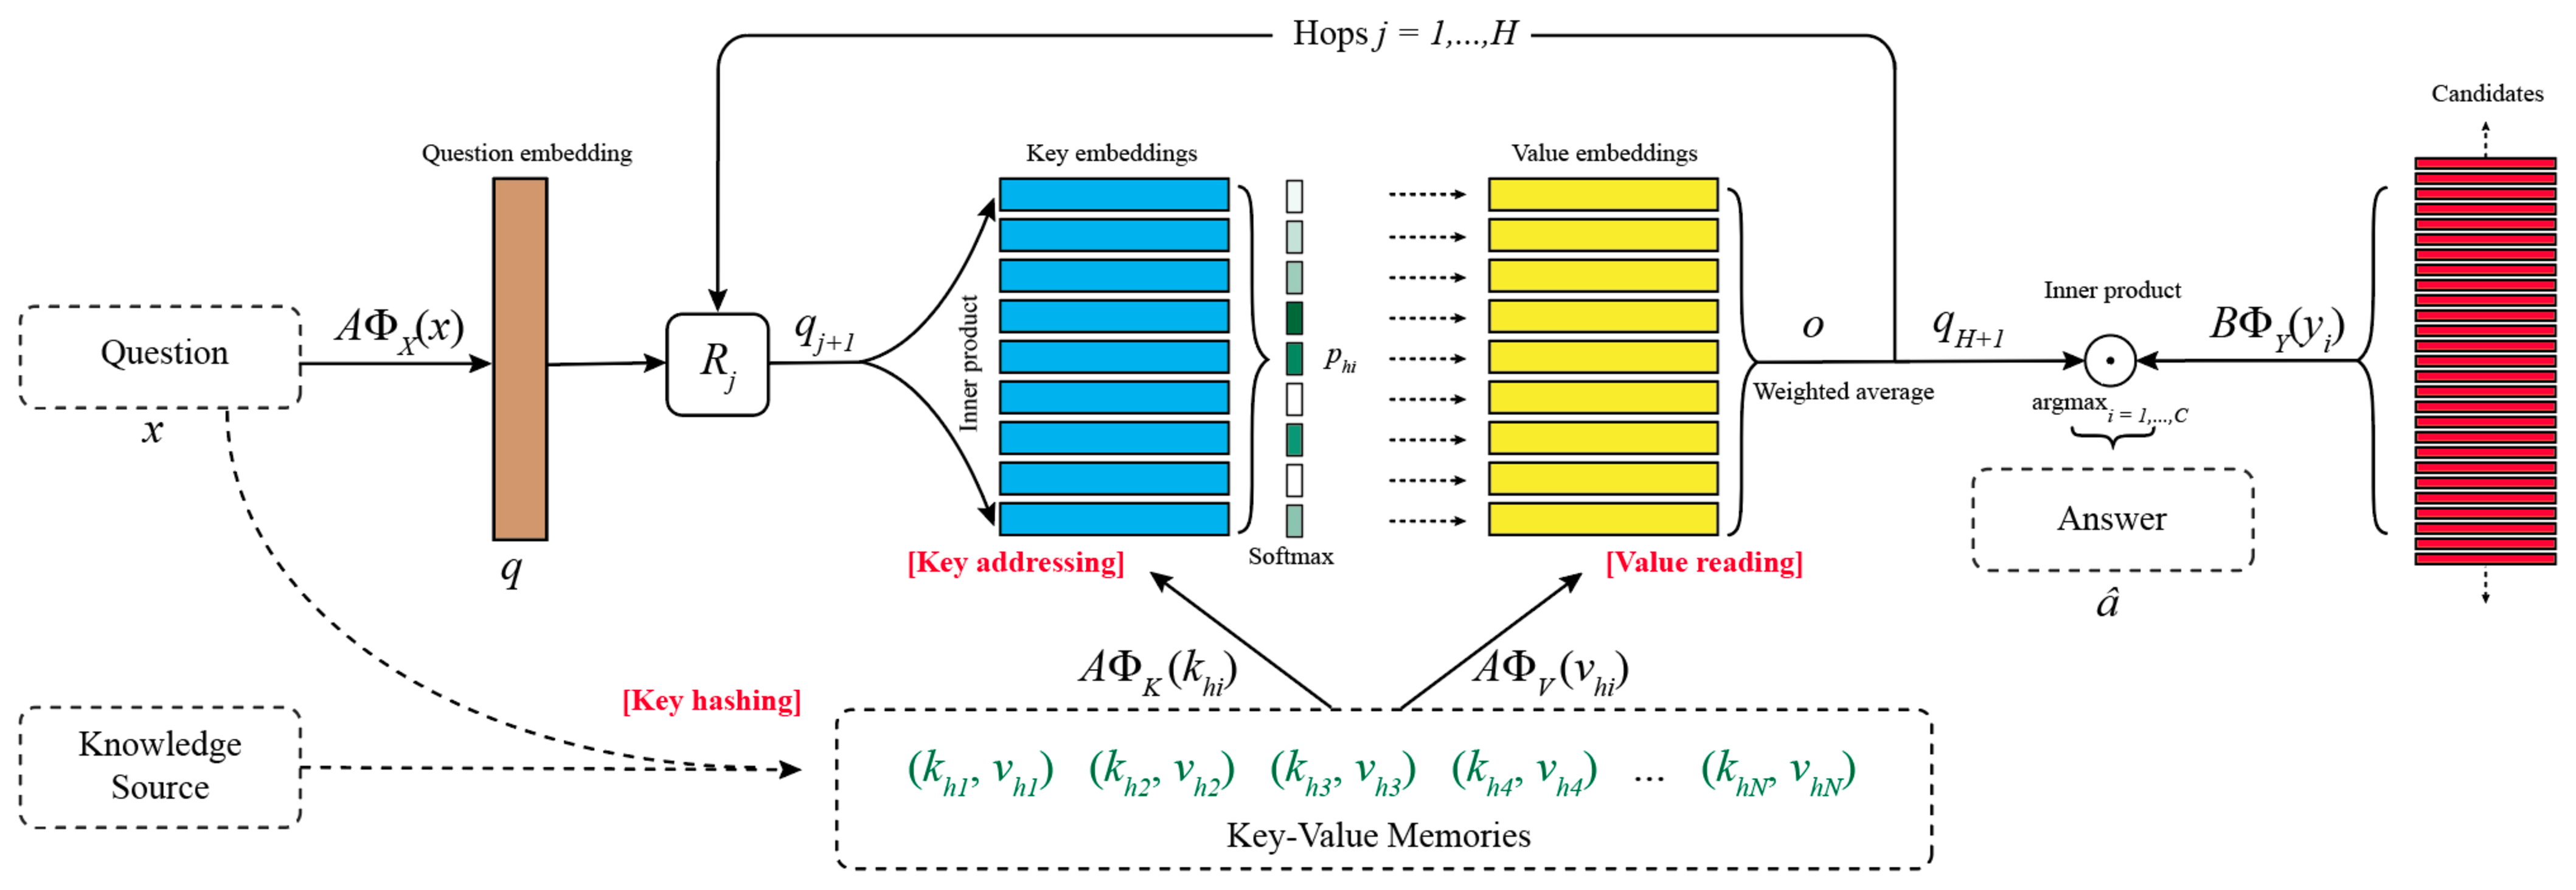
\includegraphics[width=\textwidth,keepaspectratio=true]{fig_external_memnet}
    \caption{Illustrates a Key-Value Memory Network model used in \gls{qa}. Figure 1 from \autocite{paper:journals/corr/MillerFDKBW16}}
    \label{fig:fig_external_memnet}
\end{figure}

\section{Problems}
\todo{Maybe move this part to the discussion / conclusion}
A few comments about the current generative algorithms state as we observed, but our comments may be extrapolated to \gls{ml} as a whole. Big data is currently starting to make sense in Computer Science as algorithms get incrementally more optimized, complex, and powerful. In addition to continuously improving computational power, it appears that the large amount of data produced for many years can finally deliver some premise to its potential. However, it raises new questions, such as the privacy implications. 

With its impressive 774 Million parameters, \gls{gpt2} uses a large dataset combination of News articles, Reddit comments, IRC conversations, Books, Wikipedia pages, and much more, to train the model, making it humanly impossible to review. Meaning that the model is holding potentially private information, to prove our words, we performed a potential privacy attack on \gls{gpt2} and succeed. Indeed, by merely using meta-information as input, e.g., \say{[DD/MM/YYYY, HH:MM:SS AM] <USER1>}, the model could retrieve a private conversation it once has seen. The method could also recover potential passwords, and so on.

It is essential to repeat; we believe that we are currently at the beginning of a rich potential to \gls{nlp}, particularly for text generation, as explored in this chapter and confirmed in the next, which implies additional breakthroughs within the incoming year. However, we believe that large models are meant to do good to the world, and must be under a light control to avoid bad actors damaging the image of the upcoming even more impressive technologies.

As a final note, in the scope of our project, we wish not to start a trend toward Sophist Machines, as our study may provide the tools to build algorithms able to manipulate knowledge in the way the author wants.

%\section{Common Natural Language Processing Features}
%Most of the following technics have been introduced to \gls{nlp} by the \glsfirst{ir} field. Indeed

%\subsection{Deep Learning}
%\todo{What are the problems such as bias, and how it can accumulate? Used to predict the next step. Various techniques, such as generative, recursive, etc.}

%\subsection{Unsupervised Deep Learning}
%\todo{How and when unsupervised training is helpful for NLP. What are the techniques. Talk about fine tuning and re-training.}

\chapter{Datasets}
\label{chap:datasets}

As the thesis aims at exploring a knowledge-based \gls{qa} (see Chapter \ref{chatbot:qa}) and dialogue (see Chapter \ref{chatbot:main-cats}) for chatbots combination, this chapter aims at synthesis and compare the current \gls{sota} datasets. With no surprise, we noticed that both \gls{nlp} research fields are currently in nested competitions, each field plays at defining the new \gls{sota} algorithm and dataset as baselines. In addition to \gls{nlp} breakthroughs, the competitive attitude makes the community results particularly active and exciting as new techniques, architectures, and incrementally more complex datasets releases at a monthly rate.

\section{Scope Criterions}
\label{dataset:criterions}
Even if the datasets pool base for \gls{qa} systems and Dialogues is not as exhaustive as datasets present in other \gls{nlp} fields such as \gls{lm} or even in other computer science fields, e.g., Computer Vision. The datasets at our disposal are still large, lucky to the recent interest in the fields; however, they vary significantly from each other, e.g., based on their features such as Data Sources, Quantity, or Quality. To narrow the research, as many traits are subjective and intrinsically dependent on the required tasks themselves, we defined high priority criterias.

\paragraph{Knowledge-based}
The use of \gls{kb}, such as Wikidata, been defined in the specifications as an ideal knowledge database. 

\paragraph{Open Domain}
The ability to respond to \gls{open-domain} question is meaningful to the project as we use a \gls{kb} containing by design \gls{open-domain} relations. 

\paragraph{Multiple Supporting Facts}
As an elegant \gls{kb} and \gls{open-domain} combination, \gls{mh} allows to profit from the \gls{kb} linked-data architecture to handle more complex questions.

\paragraph{Converstational}
Support of contexts to handling nested questions is particularly meaningful in our opinion as it provides to \gls{qa} additional details layers to an answer.

\paragraph{No Reasoning}
Even if mentioning supporting criteria is essential, we believe that referring to explicitly not supporting criteria is also important. In our case, we expressly do not support \gls{mr} in any manner, as reasoning could be a quantifiable task in some datasets.


\section{Question-Answering}
\label{dataset:qa}
Based on the criterions defined in (see Chapter \ref{dataset:criterions}), we made an overview Table \ref{tab:qa_overview_datasets} scoping \gls{qa} datasets related to our work. The following subsections describes the chosen datasets, ending with the worth mentioning datasets.

\subsection{ConvQuestions}
\label{dataset:convquestions}
Late 2019, ConvQuestions, a crowdsourced \gls{mh} datasets of 11'200 augmented questions on 5 domains, released with CONVEX \autocite{paper:convex}. The data augmentation is done by asking the Turker to paraphrase each question once and keeping it semantically equivalent and interchangeable. To the initial 5-turns 350 conversations, a non-reordering permutation is applied to each question and its paraphrasing. Finally, the dataset provides a Wikidata \gls{nel} to each answer.

\subsection{SimpleQuestions casted into Wikidata}
\label{dataset:simplequestions}
Initial built with crowd workers by \textit{Facebook AI Research}, SimpleQuestions\autocite{paper:journals/corr/BordesUCW15} was entity-linked to the Freebase \gls{kb} for its 108'442 (question, answer, language) triples. For their research, the AskPlatypus \autocite{paper:wikidata-benchmark} team used automatically generated mappings of 49'202 SimpleQuestions triples to Wikidata. Note that at the time of building their dataset, only 21'399 were answerable over Wikidata.

\subsection{Worth Mentioning}
Even as part of this work., the opportunity to use the following datasets was not appropriate; we believe that they are worth mentioning due to the attention they attracted lately with fine-tuned pre-trained language models (see Chapter \ref{nlp:transformers}) \gls{qa} systems.

\paragraph{Stanford Question Answering}
\label{dataset:squad}
Initially presented in 2016, \gls{squad} \autocite{paper:journals/corr/RajpurkarZLL16} was propelled by the raised of \glspl{transformer} as it was the first massively crowdsourced reading comprehension Wikipedia-based dataset with a 86.6\% human performance, making it an exciting challenge for future \gls{qa} systems. In 2018, SQuAD 2.0 \autocite{paper:journals/corr/abs-1806-03822} was released with an additional set of 50'000 unanswerable questions, adversarially similar to answerable questions present in the first version. Note that by design, \gls{squad} focuses on confusing questions, approachable by combining paraphrasing and text summarization \gls{nlp} tasks.

\paragraph{Conversational Question Answering Challenge}
\label{dataset:coqa}
Released in 2019, \gls{coqa} \autocite{paper:journals/corr/abs-1808-07042} is a \gls{mh} dataset containing 127'000 questions obtained from 8'000 conversation over 7 difference sources. With a human-performance of 88.8\% \gls{coqa} implies reading comprehension with coreference and pragmatic reasoning.

\paragraph{Question Answering in Context}
Since 2018, \gls{quac} \autocite{paper:journals/corr/abs-1808-07036} is challenging \gls{qa} system with its \gls{mh} dataset containing 100K crowdsourced evidence-based questions aiming at providing \gls{qa} in a dialog manner with context holding. Questions are designed to be open-ended, unanswerable without context and focusing on missing information.

\paragraph{Compare \gls{squad}, \gls{coqa} and \gls{quac}}
In 2019, a comparative study \autocite{paper:journals/corr/abs-1809-10735} have been conducted for the previously mention three datasets, comparing them on the basis of unanswerablility, \gls{mh}, and question abstraction.


\section{Dialogue Datasets}
\label{dataset:dialogue}
As the project scope requires a chatbot able to answer \gls{nl}, we explored the available conversational datasets. Compared to the \gls{qa} datasets (see Chapter \ref{dataset:qa}), we discovered an underrepresented field of \gls{nlp} as the presence is relatively poor. Recapitulated in the Table \ref{tab:dialogues_overview_datasets}, we focused on the datasets featuring on \gls{qa} setups and multi-domains dialogue openness. We identified a unique dataset matching our requirements and two worth mentioning datasets, reinforcing an overall subjective view implying that dialog-based \gls{nlp} research currently in standby. Indeed, it would not surprise us, as pre-trained language models have started reaching a popular peak of interest, that the field of Dialogue gains a sudden interest and challenges \gls{gpt2} \autocite{papers:gpt2}.


\subsection{Natural Questions Corpus}
\label{dataset:googlenatural}
Another jewel of 2019, with over 323'000 dialogues, \textit{Google's} Natural Questions Corpus dataset \autocite{paper:google-natural-questions} is a benchmarking approach for \gls{nl} generated answers in a \gls{qa} environment, making it particularly interesting for fine-tuned pre-trained language models like \gls{gpt2} \autocite{papers:gpt2}. Its goal is to provide an appropriate training and testing set for \gls{qa} systems, by pairing \textit{Google Search Engine}'s real user queries to a large pool of crowdsourced cross-annotations, they call \say{high quality annotations}, to guarantee answer quality over documents. Additionally, their mythology defines new metrics to evaluate answering performances. Interestingly, the dataset provides statistics, a long answer, a short answer, and an answer \gls{nel} to a Wikipedia page in most cases.

\subsection{Worth Mentioning}
The following datasets are particularly interesting from a Chatty (see Chapter \ref{chatbot:main-cats}) point of view, but no further out-of-the-box features without pre-processing or data augmentation are present. In our case, no Wikidata \gls{nel}  is available, nor the data is set explicitly in a \gls{qa} manner, making it particularly random in various contexts. However, the datasets are still impressive by their quantities and their conversational feature.

\paragraph{Twitter Conversation Triple}
This 2015 dataset uses Context-Message-Response triples as storage architecture, making it particularly interesting for parallelized training. Additionally, with its impressive 129 Million tweets tuples, it makes it the most substantial research dataset released until the time of writing. The dataset is currently combined with \gls{bleu} (see Chapter \ref{eval:bleu}) to evaluate generated dialogue, often present in the field of machine translation.

\paragraph{Ubuntu Dialogue Corpus}
\textit{Ubuntu} released its chat logs \autocite{paper:journals/corr/LowePSP15}, in 2016, containing over 1 Million multi-turns dialogues. The interest to this dataset comes from its relatively large size containing long technical contexts, and by design, it does not require exhaustive feature engineering to train over out-of-the-box.

%\paragraph{TriviaQA}
%\todo{2017. 650k question-answer-evidence triples.}

%\paragraph{MS MARCO}
%\todo{2016. (Machine Reading Comprehension). Has been used to evaluate generative models from Seq2Seq, Memory Networks, and Disciminative models. Uses Real and anonymized user queries from Bing. Context is given by a real web documents. All answers are human generated. Subsets are multiples anwsers or no as. All queries are tagged with segment informations. }

\setlength{\tabcolsep}{8pt}
\renewcommand{\arraystretch}{1.1}
\begin{landscape}
\begin{longtable}[c]{@{}lccccllll@{}}
\toprule
Datasets & \begin{tabular}[c]{@{}c@{}}Release \\ Date\end{tabular} & \begin{tabular}[c]{@{}c@{}}Nested \\ Questions\end{tabular} & Hops           & \begin{tabular}[c]{@{}c@{}}Open \\ Domain\end{tabular} & Queries & Docs                                                  & Query Source                                                                                                                                            & Answer Type                                                    \\* \midrule
\endhead
%
\bottomrule
\endfoot
%
\endlastfoot
%
ConvQuestions                                                                 & 2019                                                    & \textbf{Yes}                                                & \textbf{Multi} & \textbf{5}                                           & 11K     & 350                                                   & \textbf{Wikidata}                                                                                                                                 & Spans                                                          \\
\begin{tabular}[c]{@{}l@{}}Google \\ Natural Questions \\ Corpus\end{tabular} & 2019                                                    & No                                                          & Single         & \textbf{Yes}                                           & 323K    & ??                                                    & Wikipedia                                                                                                                                         & Spans                                                          \\
SQuAD 2.0                                                                     & 2018                                                    & No                                                          & Single         & \textbf{Yes}                                           & 151K    & 853                                                   & Wikipedia                                                                                                                                         & \begin{tabular}[c]{@{}l@{}}Spans, \\ Unanswerable\end{tabular} \\
CoQa                                                                          & 2018                                                    & \textbf{Yes}                                                & Single         & \textbf{Yes}                                           & 127K    & 8K                                                    & \begin{tabular}[c]{@{}l@{}}Children’s Stories, \\ Literature, \\ Mid/High School Exams, \\ News, \\ Wikipedia, \\ Reddit, \\ Science\end{tabular} & \begin{tabular}[c]{@{}l@{}}Spans, \\ Unanswerable\end{tabular} \\
QuAC                                                                          & 2018                                                    & \textbf{Yes}                                                & Single         & \textbf{Yes}                                           & 100K    & 14K                                                   & Wikipedia                                                                                                                                         & \begin{tabular}[c]{@{}l@{}}Spans, \\ Unanswerable\end{tabular} \\
HotpotQA                                                                      & 2018                                                    & No                                                          & \textbf{Multi} & \textbf{Yes}                                           & 113K    & 591                                                   & Wikipedia                                                                                                                                         & Spans                                                          \\
DuReader                                                                      & 2018                                                    & No                                                          & Single         & \textbf{Yes}                                           & 300K    & 1.5M                                                  & Web Search                                                                                                                                        & Spans                                                          \\
TriviaQA                                                                      & 2017                                                    & No                                                          & \textbf{Multi} & \textbf{Yes}                                           & 650K    & 95K                                                   & Trivia                                                                                                                                            & Spans                                                          \\
RACE                                                                          & 2017                                                    & No                                                          & Single         & No                                                     & 97K     & 28K                                                   & Mid/High School Exams                                                                                                                             & \begin{tabular}[c]{@{}l@{}}Multiple \\ choice\end{tabular}     \\
Narrative QA                                                                  & 2017                                                    & No                                                          & \textbf{Multi} & \textbf{Yes}                                           & 47K     & 1.6K                                                  & \begin{tabular}[c]{@{}l@{}}Movie Scripts, \\ Literature\end{tabular}                                                                              & Spans                                                          \\
SearchQA                                                                      & 2017                                                    & No                                                          & \textbf{Multi} & \textbf{Yes}                                           & 140K    & 6.9M                                                  & Jeopardy                                                                                                                                          & Spans                                                          \\
NewsQA                                                                        & 2017                                                    & No                                                          & Single         & \textbf{Yes}                                           & 100K    & 10K                                                   & News                                                                                                                                              & Spans                                                          \\
\begin{tabular}[c]{@{}l@{}}QAngaroo \\ WikiHop\end{tabular}                   & 2017                                                    & No                                                          & \textbf{Multi} & \textbf{Yes}                                           & 51K     & 528K                                                  & \textbf{Wikidata}                                                                                                                                 & Spans                                                          \\
\begin{tabular}[c]{@{}l@{}}QAngaroo \\ MedHop\end{tabular}                    & 2017                                                    & No                                                          & \textbf{Multi} & No                                                     & 2.5K    & 528K                                                  & \begin{tabular}[c]{@{}l@{}}Medline, \\ Drugbank\end{tabular}                                                                                      & Spans                                                          \\
\begin{tabular}[c]{@{}l@{}}CNN / \\ Daily Mail\end{tabular}                   & 2016                                                    & No                                                          & Single         & \textbf{Yes}                                           & 1.4M    & \begin{tabular}[c]{@{}l@{}}93K / \\ 220K\end{tabular} & News                                                                                                                                              & Spans                                                          \\
Children’s Book                                                               & 2016                                                    & No                                                          & Single         & No                                                     & 688K    & 108                                                   & Children’s stories                                                                                                                                & \begin{tabular}[c]{@{}l@{}}Multiple \\ Choice\end{tabular}     \\
SQuAD                                                                         & 2016                                                    & No                                                          & Single         & \textbf{Yes}                                           & 108K    & 536                                                   & Wikipedia                                                                                                                                         & Spans                                                          \\
MS MARCO                                                                      & 2016                                                    & No                                                          & Single         & \textbf{Yes}                                           & 100K    & 200K                                                  & Web Search                                                                                                                                        & \begin{tabular}[c]{@{}l@{}}Spans, \\ Unanswerable\end{tabular} \\
SelQA                                                                         & 2016                                                    & No                                                          & Single         & \textbf{Yes}                                           & 8K      & 486                                                   & Wikipedia                                                                                                                                         & Spans                                                          \\
INFOBOXQA                                                                     & 2016                                                    & No                                                          & Single         & \textbf{Yes}                                           & 15K     & 150                                                   & Wikipedia                                                                                                                                         & Spans                                                          \\
WikiQA                                                                        & 2015                                                    & No                                                          & Single         & \textbf{Yes}                                           & 3K      & 29K                                                   & \begin{tabular}[c]{@{}l@{}}Wikipedia, \\ Web Search\end{tabular}                                                                                  & \begin{tabular}[c]{@{}l@{}}Sentence \\ Selection\end{tabular}  \\
SimpleQuestions                                                              & 2015                                                    & No                                                          & Single         & \textbf{Yes}                                           & 109K    & 6K                                                    & \textbf{Freebase}                                                                                                                                 & Spans                                                          \\
bAbI tasks 1 to 6                                                             & 2015                                                    & No                                                          & \textbf{Multi} & \textbf{Yes}                                           & 6M      & ??                                                    & ??                                                                                                                                                & Spans                                                          \\
MCTest                                                                        & 2013                                                    & No                                                          & Single         & \textbf{Yes}                                           & 2.6K    & 660                                                   & Children’s stories                                                                                                                                & \begin{tabular}[c]{@{}l@{}}Multiple \\ Choice\end{tabular}     \\* \bottomrule
\caption{Overview of Question Answering Datasets. In bold the features identified to be meaningful for the Thesis.}
\label{tab:qa_overview_datasets}\\
\end{longtable}
\end{landscape}


\setlength{\tabcolsep}{7pt}
\renewcommand{\arraystretch}{1.1}
\begin{landscape}
\begin{longtable}[c]{@{}lcccrrll@{}}
\toprule
Datasets                                                                      & \begin{tabular}[c]{@{}c@{}}Release \\ Date\end{tabular} & QA           & \begin{tabular}[c]{@{}c@{}}Open \\ Domain\end{tabular} & Dialogues     & Utterances & Query Source    & Dialogue Type            \\* \midrule
\endhead
\bottomrule
\endfoot
\endlastfoot
\begin{tabular}[c]{@{}l@{}}Google \\ Natural Questions \\ Corpus\end{tabular} & 2019                                                    & \textbf{Yes} & \textbf{Yes}                                           & 323K & ??         & Wikipedia       & Human to Human,          \\
Reddit                                                                        & 2017                                                    & No           & \textbf{Yes}                                           & 54M  & ??         & Comments        & Human to Human           \\
DSTC4                                                                         & 2016                                                    & \textbf{Yes} & No                                                     & 35            & ??         & Chat logs       & Human to Human           \\
Twitter Triplets Corpus                                                       & 2015                                                    & No           & \textbf{Yes}                                           & 129M & 87M        & C-M-R Tweats    & Human to Human, blogging \\
Ubuntu Dialogue                                                               & 2015                                                    & No           & \textbf{Yes}                                           & 1M   & 7M         & Chat logs       & Human to Human           \\
Sina Weibo                                                                    & 2015                                                    & No           & \textbf{Yes}                                           & 4.4M & 8.8M       & Posts, Comments & Human to Human, blogging \\
DSTC2                                                                         & 2014                                                    & No           & No                                                     & 3K            & 24K        & Chat logs       & Human to Computer        \\
DSTC3                                                                         & 2014                                                    & \textbf{Yes} & No                                                     & 2.3K          & 15K        & Chat logs       & Human to Computer        \\
DSTC1                                                                         & 2013                                                    & \textbf{Yes} & No                                                     & 15K           & 210K       & Chat logs       & Human to Computer        \\
Twitter Corpus                                                                & 2010                                                    & No           & \textbf{Yes}                                           & 1.3M & 3M         & Posts, Tweats   & Human to Human, blogging \\
OpenSubtitles                                                                 & 2009                                                    & No           & \textbf{Yes}                                           & 70M  & ??         & Movies          & Human to Human           \\* \bottomrule
\caption{Dialogues Datasets Overview. In bold the features identified to be meaningful for the Thesis.}
\label{tab:dialogues_overview_datasets}\\
\end{longtable}
\end{landscape}


\chapter{Evaluation}
\label{chap:evaluation}

\section{Generative}
\todo{Not a lot of work has been done in the domain of computer generated text, taking appart machine translation. So far I found a paper (GLTR: Statistical Detection and Visualization of Generated Text) that talks about a technic to detect generated content. And I found an article about the Readers’ perception of computer-generated news(: Credibility, expertise, and readability) which says that people like to read computer generated content because it's what it is, and humans are amazed about it, the long term have to be explored.}
\paragraph{BLEU}
\todo{The Bilingual evaluation understudy was originally made to measure machine translation and now is used for Natural language generation. The goal is to compare the machine generated output text string to its expected output, the algorithm is fast and easily computable compared to human translators. Plus, it's benchmarkable. However, it's not made to take the meaning of the sentence into account (attention), it's not taking into account the sentence structure, it's doesn't work with rich languages and it doesn't take into account how humans are actually interpreting the sentences. Basically to used only in the machine translation context to evaluate an entire corpus.}
\paragraph{ROUGE}
\todo{Adaptation from BLUE to focus on the recall instead of Precision. It checks the the reference translation to the output.}

performances

\section{QA Systems}
\section{Generative Systems}
\section{Conversational Agents}

%\chapter{Problems}
\label{chap:problems}

\todo{Generative: Exfiltrating copyright notices, news articles, and IRC conversations from the 774M parameter GPT-2 data set. Sofist Machines}

%\chapter{State of the Art Sumup}
\label{chap:sota-conlusions}

\section{Performances}
\todo{POS tagging}
\todo{Parsing}
\todo{Named-Entity Recognition}
\todo{Named-Entity Linking}
\todo{Semantic Role Labeling}
\todo{Question Answering}
\todo{Dialogue Systems}
\todo{Contextual Embeddings}

\section{Chatbots}

\section{}
%\chapter{State of the art}
\label{chap:state-of-the-art}









%\chapter{Language Models}
\label{chap:language-models}
%\chapter{Generative Models}
\label{chap:generative-models}
%\chapter{Machine Understanding \& Reasoning}
\label{chap:mu_mr}
%\chapter{Question Answering Systems}
\label{chap:qa}
%\chapter{Zero-Shot Learning}
\label{chap:zero-shot-learning}

\cleardoublepage

%PART 3
\part{Design and realization}
\chapter{Analysis}
\label{chap:analysis}

In this chapter, we analyze the \gls{sota} (see Part \ref{part:sota}) to define the scope of the \gls{poc} and add additional knowledgable details to project specifications as our initial understanding of the thesis subject increased. As a kickoff to research the \gls{sota} and for the analysis, in addition to peer consulting with our lab colleagues in the field of \gls{nlp}, we used curated lists e.g., awesome-nlp on Github \autocite{website:awesomenlp-github}. The knowledge accumulation started naturally to chain as we began to read papers mentioned in other papers.

\section{Rescoping and Motivations}
\label{analysis:rescoping}
Extrapolated from the \gls{sota} part \ref{part:sota}, we present in this section the process held to get to the final project scope based on the accumulated knowledge thru \gls{nlp} \gls{sota} exploration.

\subsection{Initial Project}
Our research initially started as a satellite to the \textit{AI-News} project (see Chapter \ref{intro:icosys}), which is currently using a Retrieval approach (see Chapter \ref{chatbot:retrieval}) combined with an intents and entities extraction, to return highly pondered recent articles from an elastic search in a Ruled-Based chatbot (see Chapter \ref{chatbot:rulebased}) format. The \textit{AI-News} project scoped our research indirectly toward finding solutions to bring \gls{qa} systems to the field of journalism; however, it early rescoped to open domain knowledge as the \gls{wikidata} \gls{kb} provides crowdsourced general knowledge. Additionally to the \gls{qa} scope, the specification implies \gls{nl} answers generation. We intended to build a \gls{qa} system to generate \gls{bleu} approved corpora based on the \gls{wikidata} \gls{kb}, then compare them to \gls{squad} benchmarking (see Chapter \ref{dataset:squad}), with the ultimate purpose to compare Pre-Trained Language Models such as BERT on your new dataset. As the starting point, we decided to bootstrap our project with \gls{sota} related papers filtered by code availability and reproducibility.

\subsection{Initial Ideas}
To achieve our initial project, we brainstormed the following ideas. Indeed, we expected to explore in detail the field of \gls{qa} evaluation in particular Oracle-based solutions, oracles are particularly meaningful in our context as we would use \gls{wikidata} as an oracle. Additionally, we planned to explore in more detail the effects of fine-tuning pre-trained language models such as \gls{bert}, with the intent to create a challenging dataset. Based on a finite state grammar, our evaluation would initially generate a set of 100'000 \gls{wikidata} \gls{spo}-based questions and using word-embedding similarity feature to paraphrase those questions to increase complexity. We even discuss an additional feature to generate \gls{qa} multi-turns conversations (see Chapter \ref{chatbot:context}) by self-training a model with an \gls{al} approach.


\subsection{Second Brainstorming Iteration}
As research progressed, we took the party that we did not want to be just another benchmarking system for \gls{qa} systems, similarly to our initial decision not to become an nth fine-tuned pre-trained language model. As a result, our second brainstorming iteration brought quite a new scope to the project. Indeed, we focused mainly on a \gls{mh} multi-turns conversations approach, by aiming at building an interactive and proactive reversed Akinator-like \autocite{website:akinator} \gls{qa} system. The system would use a \say{child} learning approach as the model itself starts with no knowledge, and incrementally learns new knowledge by interacting with users. The goal is to teach the model to retrieve information from a \gls{kb} by itself. The game consists of a randomly selected \gls{wikidata} entity as the answer, and the user is requested to help, via a gamified conversational interaction, the bot to build a path in \gls{wikidata}, as it asks questions to the user. The proactive ability would a generative approach to scenario-based chatbot like HelloJam \autocite{website:hellojam}, which uses intermediary steps as a proactive approach. As a training bootstrap, we initially planned to build a conversational simulator using multi-hop datasets such as ConvQuestions, \gls{squad}, or \gls{quac}.


\section{Third Brainstorming Iteration}
Quickly, the previous brainstorming iteration raised problems such as the truth user interest for such games and the bias induced by genuine or intentional human errors, without mentioning the pre-processing needed to build a meaningful training dataset, but we kept some ideas. We believed that the \gls{mh} multi-turns conversations are an essential feature to our work, combined with the interactive and proactive approach between the bot and the user, which is a particularly exciting application in the \gls{nlp} field. We then suggested a new shift in the project scope to build \gls{nl} \gls{qa} chatbot allowing the user to interact with the conversation and the knowledge in a meaningful manner. The goal is to provide the user the ability to check returned answers with facts and correct them on the fly if needed. Additionally, we wanted to add a multi-model approach to handle virtual personalities as a flavor of personalization to the user.


\subsection{Final Brainstorming Iteration}
The project scope shifted one last time. We noticed that the applications in the field of \gls{qa}, and \gls{generative} chatbot are extensive, and it appeared that it is possible to find a paper already mentioning, even lightly, what we believed original ideas. As a contradiction, we decided at aiming directly at the roots of \gls{qa} and \gls{generative} systems as a whole. To do so, we kept the multi-hops reasoning, multi-turn conversations, and the \gls{wikidata} \gls{kb} as constraints to the project. Indeed, we did not want to be just another \gls{transformer} related project trying to define the new baseline. Our resources at disposal were limited, and we wanted to take a new approach by exploring an original technique for \gls{qa}, in particular, Sub-Knowledge Graphs. To achieve our latest project, we examined existing \gls{sota} systems providing, in addition to the paper, a runnable code to get started. We initially aimed at incrementally improve the original work to impact the \gls{nlp} field. Our first step was to reproduce the results; then, the second step was to retrain and provide additional value to the original work. And finally, adapt the initial project to the News field with few tweaks. 

\section{Question-Answering Systems Choices}
Based on the \gls{sota} (see Part \ref{part:sota}) and the previous rescoping section \ref{analysis:rescoping}, we aim at building a \gls{qa} \gls{mh} and multi-turn converstational chatbot using sub-graphs from \gls{wikidata}. We found a unique direct competitor to our work, and we are using its baselines and nested baselines to compare our work.

\subsection{Competitors}
We initially explored \gls{qa} system using the \gls{wikidata} \gls{kb} by default, and providing the must-have features defined in the project scope, our research revealed a unique candidate and two related candidates as they define the baseline of our main candidate.

\paragraph{CONVEX}
As our direct competitor, CONVEX \autocite{paper:convex} (see Chapter \ref{eval:convex}) extracts sub-graph from \gls{wikidata} \gls{kb}. It employs the sub-graphs as context holders and uses them to answer context-related questions via a frontier algorithm. It finally extends the context-graph with the new answers, making the graph more precise at answering detailed questions.

\paragraph{qAnswer and Platypus}
Both \gls{qa} systems are using a template-based model (see Chapters \ref{eval:qanswer} and \ref{eval:platypus}), and are defined as baseline in our main candidate and they are designed to for \gls{wikidata} queries. Note that they are \gls{sh} and trained on the SimpleQuestions dataset, which we also plan to use as a fair evaluation.


\subsection{Datasets}
Our initial predetermined dataset was \gls{squad} due to its popularity and its public leaderboard, as it would have been a pleasant additional comparison to our work. However, \gls{squad} is designed to answer fact-based questions with a span extracted from the given context paragraph, often implying a mismatch with fact entities such as in the \gls{wikidata} \gls{kb}. It is also a reason for CONVEX to not evaluate on this dataset, similarly to qAnswer and Playtypus. Finally, in the scope of the project, we did not plan to adapt the \gls{squad} dataset for \gls{wikidata}-based \gls{qa} systems.

\paragraph{ConvQuestions}
As descried in Evaluation Chapter (see \ref{eval:convex}), CONVEX \autocite{paper:convex} is design to use the ConvQuestions dataset (see Chapter \ref{dataset:convquestions}), which is a multi-turn conversations and \gls{mh} \gls{qa} crowdsourced dataset. CONVEX uses also this dataset with its baselines providing an initial evaluation for all three competitors.

\paragraph{SimpleQuestions}
As presented in the Dataset Chapter (see \ref{dataset:simplequestions}), SimpleQuestions has a \gls{wikidata} \gls{kb} adaptation provided by Playtpus authors \autocite{paper:InProceedingsPellissier-Tanon.P-TD-d-ACM-S_18}. This dataset will be used to benchmark our system in addition to all three competitors, as a fair approach to evaluate \gls{sh} systems on \gls{sh} design datasets.

\subsection{Benchmarking}
To measure and compare our work, we will set up two benchmarks. The first benchmark will evaluate the \gls{sh} capabilities of each competitor on the \gls{wikidata} adapted SimpleQuestions dataset. The second benchmark is focusing on the \gls{mh} and multi-turn conversations capabilities from each competitor. As qAnswer and Platypus are not designed for multi-turn conversations, we will extend them with CONVEX and our work during the multi-turn task, as both projects can work on top of other algorithms (see the next Chapter \ref{chap:graphqa}).



\section{Texts Generation Choices}
We plan to used two \gls{sota} pre-trained \gls{lm} in there vanillia large format, \gls{bert} \autocite{paper:devlin-etal-2019-bert} and \gls{gpt2} \autocite{papers:gpt2}, for our text generation \gls{nlp} task. \gls{bert} will be used as a text filler for the SPOs paths extracted complementary to the answer from the \gls{wikidata} Sub-Knowledge Graphs. \gls{gpt2} will be used as a complementary facts generator to the answer.

\paragraph{Evaluation}
We consider \textit{Google's} dataset (see Chapter \ref{dataset:googlenatural}) as promising; however, we did not plan to evaluate our generated \gls{nl} answers on this dataset as the project planning is too tight to include this protocol. We instead, we will assess the dialogues generated manually. An evaluation idea would be to run a campaign with 10 to 20 users evaluating 10 to 20 questions, using the evaluation tags: \say{Good}, \say{Neutral}, or \say{Bad}. However, this dataset is worth considering for future extended work. 

\section{Final Project Scope}
GraphQA, as we name it, is a \gls{qa} Sub-Knowledge Graphs chatbot using  the \gls{wikidata} \gls{kb} database. It extracts answers to questions from a complete \gls{linked-data} database by extracting small portions of the main database and manipulates it as a graph. The graph manipulation implies context holding, extension, and refining. Initially, based on CONVEX, we plan to improve their \gls{ir}-based answering to the first answer, as it is their bottleneck, which is particularly sensitive as it defines a successful anchor to a conversation-driven \gls{qa}. We wish to also explore sub-graph capabilities with temporally depend contexts, and their overall performances. Additionally, \gls{nl} capabilities must be present by combining two complementary pre-trained language models.

\subsubsection{Expected Features}
We define below the features we expect to be present in GraphQA as a \gls{mh} Conversational \gls{qa} Chatbot.

\begin{itemize}
    \setlength\itemsep{0em}
    \item Extract question keywords.
    \item Extract a question-related Sub-Knowledge Graph.
    \item Compute the answer from the Sub-Knowledge Graph.
    \item Extract an SPO Tuple meaningful to the question.
    \item Prune the Sub-Knowledge Graph of context meaningless elements
    \item Generate a \gls{nl} answer from the SPO Tuple.
    \item Extend the \gls{nl} generate an answer with additional facts.
    \item Extend the Sub-Knowledge Graph with new questions.
\end{itemize}


\subsubsection{Nice to have}
As we do not expect to have the time to add additional features to the primary features described in the above subsection. We are mentioning some features that we would like to see in the project one day. Note that \gls{kb} databases are by design only as good as the data the relations they hold, which is limited also by the employed schemas, implying if the reasoning information such as quantities were not manually referenced into the database, the answer is impossible to retrieve.

\begin{itemize}
    \setlength\itemsep{0em}
    \item Give the ability to merge pre-generated sub-graphs.
    \item Use of multiple modules to manage different processes.
    \item Include reasoning modules such as inductive logic or quantification.
    \item Provide an auto-correct tool to users.
    \item Provide an auto-complete tool to users.
    \item Provide a paraphrasing tool to generated answers.
    \item Use the multilingual \gls{wikidata}'s propriety paraphrase into a translation.
    \item Use \gls{wikidata}'s multi-properties to paraphrase questions and answers.
    \item Handle pre-built sub-graphs for particular subjects such as Articles, Countries, Movies, or Famous People
    \item Track users custom sub-graphs to track the overall context.
    \item Use consensus-based modules to complementarily provide the best answers.
    \item Show visually to users their sub-graph generation
    \item Provide on-the-fly tools to modify sub-graphs.
\end{itemize}



\section{CONVEX Q0 Solutions}
As mentioned in previous sections and represented on the Figure \ref{fig:fig_high_level_convex_architecture_analysis}, CONVEX \autocite{paper:convex} has an issue with the first answer. The issue has been briefly explored and confirmed in the CONVEX paper. Indeed, for a0 (the initial answer), CONVEX uses a proprietary \gls{ner} system, TAGME \autocite{paper:CIKM-2010-FerraginaS}, as its \gls{wikidata} entities identify system. Then places into an empty a subgraph returned entities with their relation extracted from the \gls{wikidata} \gls{kb}. This process is solely relying on a TAGME to answer the initial question, which are often interpreted as lucky guesses. As one of our main contributions, we want to fix this issue, and to do so, we propose five different solutions, including a naive one. 

\begin{figure}[H]
    \centering
    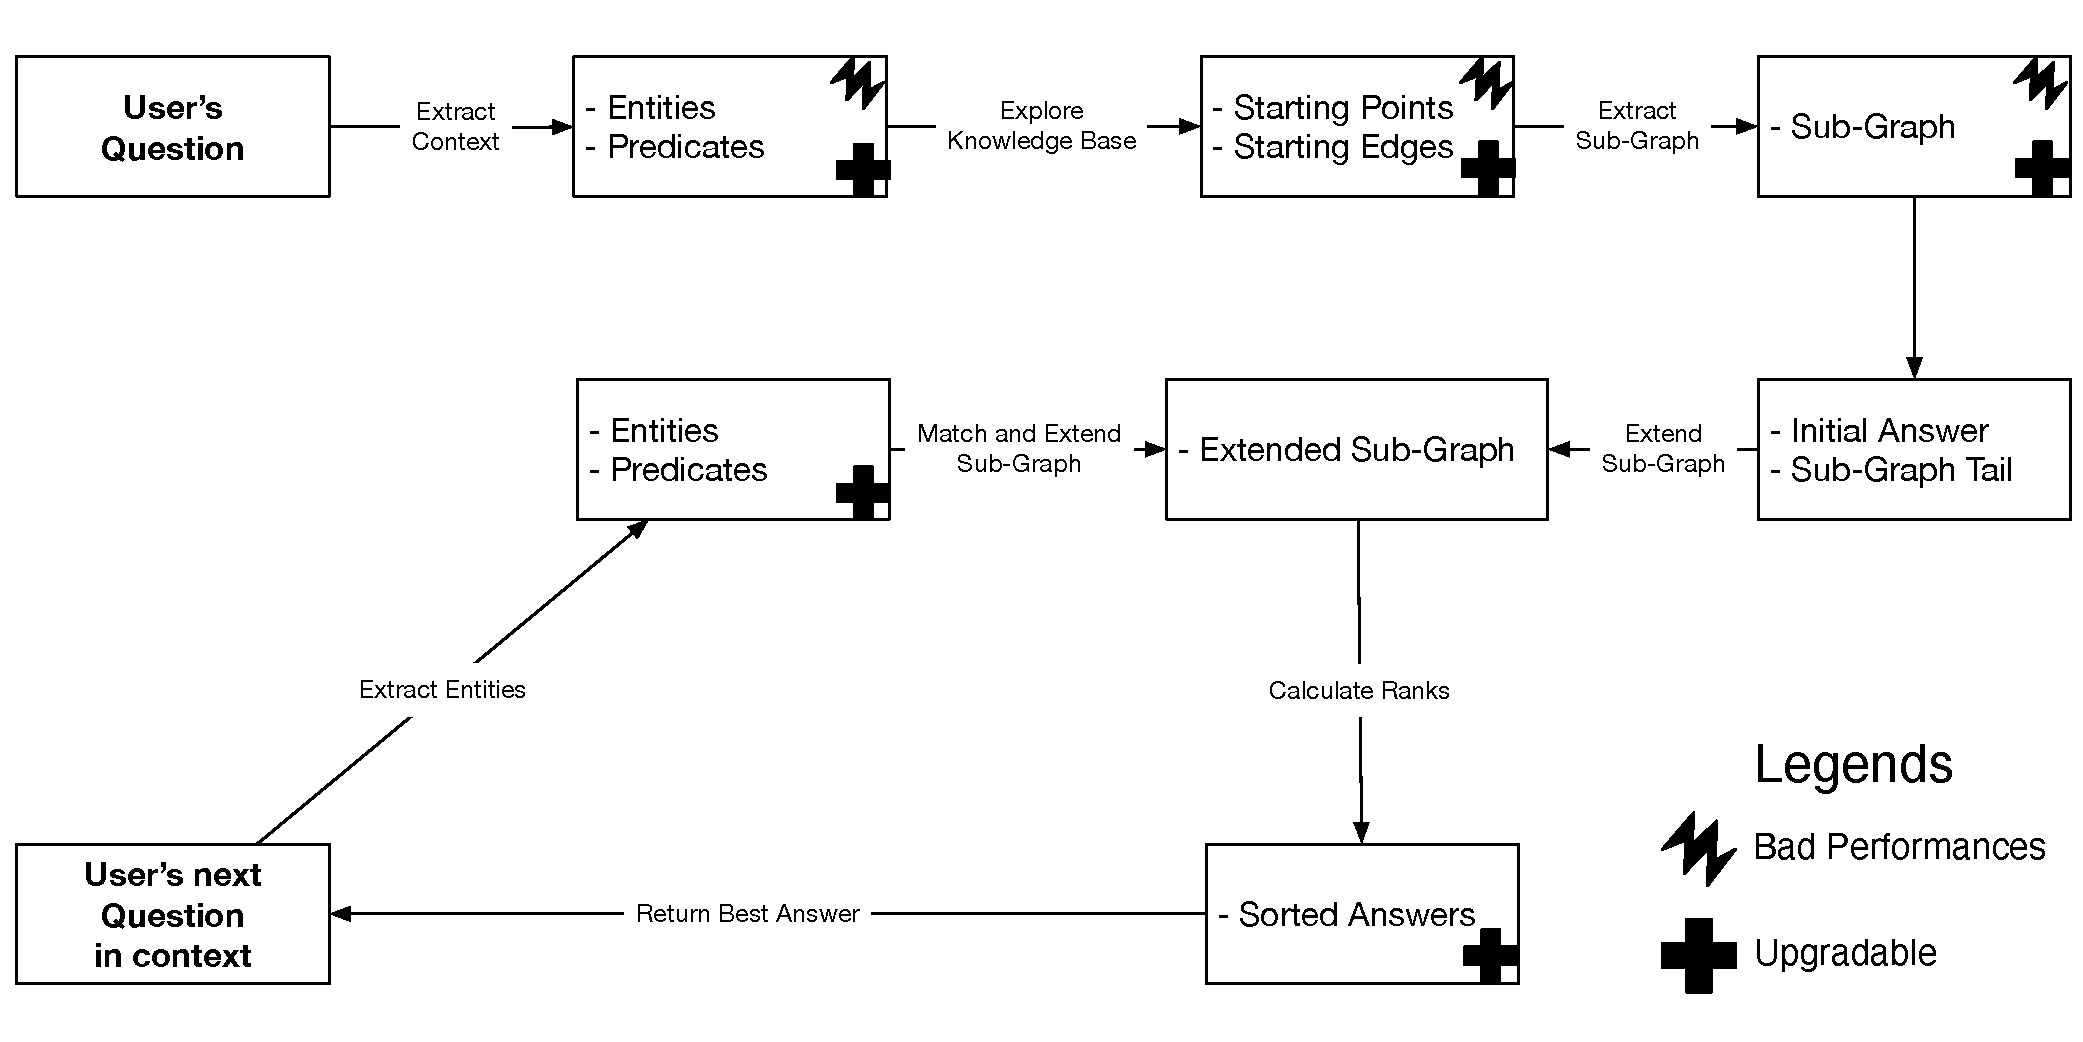
\includegraphics[width=\textwidth,keepaspectratio=true]{fig_high_level_convex_architecture_analysis}
    \caption{Illustrative representation of the high level CONVEX architecture. the diagram includes the identified part having bad performances, and shows the upgradable components.}
    \label{fig:fig_high_level_convex_architecture_analysis}
\end{figure}

\subsection{0th Solution: Naive Approach}
Our naive approach is to use text summarization to extract relevant information and build the initial sub-knowledge graph by matching the entities present in the \gls{wikidata} \gls{kb}. It is indeed not an impressive approach by at least we have control over the extracted data, and we can study the related induced behaviors, then tune the system with additional models.

\subsection{1st Solution: BiDAF++}
\label{analysis:bidaf}
The BiDAF++ model, presented with \gls{quac} \autocite{paper:journals/corr/abs-1808-07036}, is based on BiDAF \autocite{paper:journals/corr/SeoKFH16} augmented with self-attention \autocite{paper:journals/corr/abs-1710-10723} and ELMo \autocite{paper:journals/corr/abs-1802-05365}, and particularly used as non-\gls{transformer} baseline on multiple \gls{qa} datasets. We could explore training on multiple dataset such as Google's Natural Questions Corpus \autocite{paper:google-natural-questions}, ConvQuestions \autocite{paper:convex}, CoQA \autocite{paper:journals/corr/abs-1808-07042} and NewsQA \autocite{paper:journals/corr/TrischlerWYHSBS16}. The model would provide us the answers to the questions, and we would build the initial sub-graph based on the matched entities id found in the question and the entity found as the answer.

\subsection{2nd Solution: Multi-task learning}
Multi-task learning for large scale \gls{kb} \autocite{paper:2019arXiv191005069S} is by design handling the conversational \gls{qa} format, making it particularly appealing to our project. The techniques model trained to parse questions and point them into the \gls{kb} via pointers, which avoids the propagation of errors and simultaneously exploits the pointer property to share the linked information.

\subsection{3rd Solution: Knowledge Graph Embedding}
Knowledge Graph Embedding \autocite{paper:2019arXiv191102168W} is model trained to locate entities (subject) and predicates individually in a \gls{kg} and then predict the tail (object). However, this technique, as described by the authors, works only for simple questions, which conflicts with our \gls{mh} constraint, implying to extend the model capabilities to \gls{mh} handling. 

\subsection{4th Solution: Fine-tuned Pre-trained Language Model}
Even if we do not expect to use this solution, it is still worth mentioning. Indeed, the final solution would be to fine-tune a transformer-based model on multiple \gls{qa} datasets similarity mentioned in the 1st solution above (see Subsection, \ref{analysis:bidaf}).


\subsection{Our representation in the Chatbot Cartography}
To conclude this chapter, we updated the chatbots cartography as defined in the chatbot state-of-the-art chapter (see \ref{chatbot:cartography}) to illustrate our position. (See Figure \ref{fig:fig_chatbot_cartography_graphqa})

\begin{figure}[H]
    \centering
    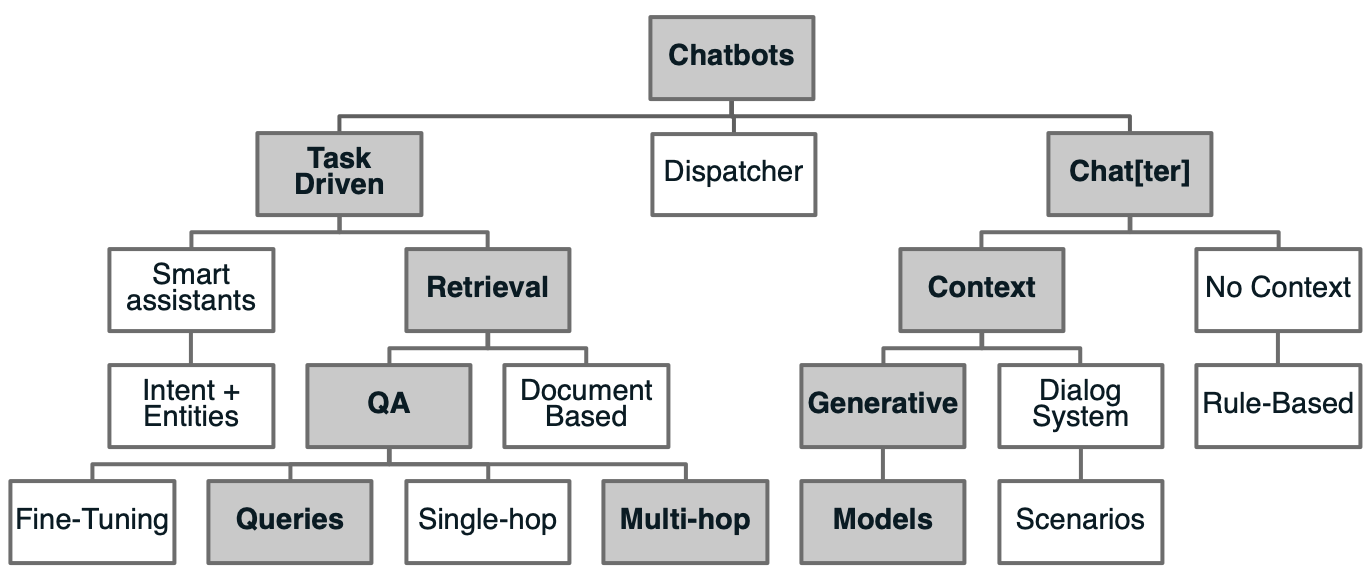
\includegraphics[width=\textwidth,keepaspectratio=true]{fig_chatbot_cartography_graphqa}
    \caption{Represents GraphQA's positions in the chatbots cartography as defined in the chatbot state-of-the-art chapter.}
    \label{fig:fig_chatbot_cartography_graphqa}
\end{figure}


\chapter{Project Management}
\label{chap:dev-project-management}



\chapter{Architecture}
\label{chap:architecture}

Multi models from presentation

Grounded approch with zero learning similar results


\chapter{GraphQA}
\label{chap:graphqa}

As stated in the analysis (see chapter \ref{chap:analysis}), GraphQA planned to be a straight forward approach for improving the CONVEX \autocite{paper:convex} prototype on Q0. As a second step, the project would aim toward \gls{nl} generated answers based on the Sub-Knowledge Graphs. As this chapter goes, we could not go as planned during the analysis (see Chapter \ref{chap:analysis}) due to CONVEX complications encountered. However, to our relief, we could bounce back and produce original work. Our final approach started with the naive solution proposed during the analysis (see Chapter \ref{analysis:naive}) and combined it with exciting features we particularly thought meaningful from our analytical brainstorming (see Chapter \ref{analysis:rescoping}). Indeed, in addition to our well defined Multi-Turn Conversations, \gls{mh}, and \gls{wikidata} \gls{kb} Sub-Knowledge Graphs scoped features, we are exploring a \gls{gl} approach by orchestrating various specialized \gls{nlp} models as a global \gls{zero-shot} learning approach for \gls{nl} \gls{qa} chatbots. Finally, we keep the same evaluation settings, as stated in the analysis (see Chapter \ref{analysis:benchmarking}), including the ability for GraphQA to works on top of other \gls{qa} systems.

\section{GraphQA Architecture}
We aim at highlighting in this section the High-Level Architecture evolution from the initial analysis-based scope to our current architecture.

\subsection{Initial Architecture}
\label{graphqa:initial}
As represented in Figure \ref{fig:fig_high_level_convex_architecture_graphqa}, the initial approach for GraphQA was to enhance the CONVEX architecture for the Q0 question (see Chapter \ref{analysis:convexq0}), and then plug a \gls{nl} generator for answers. Finally, the second step was the upgrade of additional CONVEX modules and suggest new use cases to the project, such as a News extension.

\begin{figure}
    \centering
    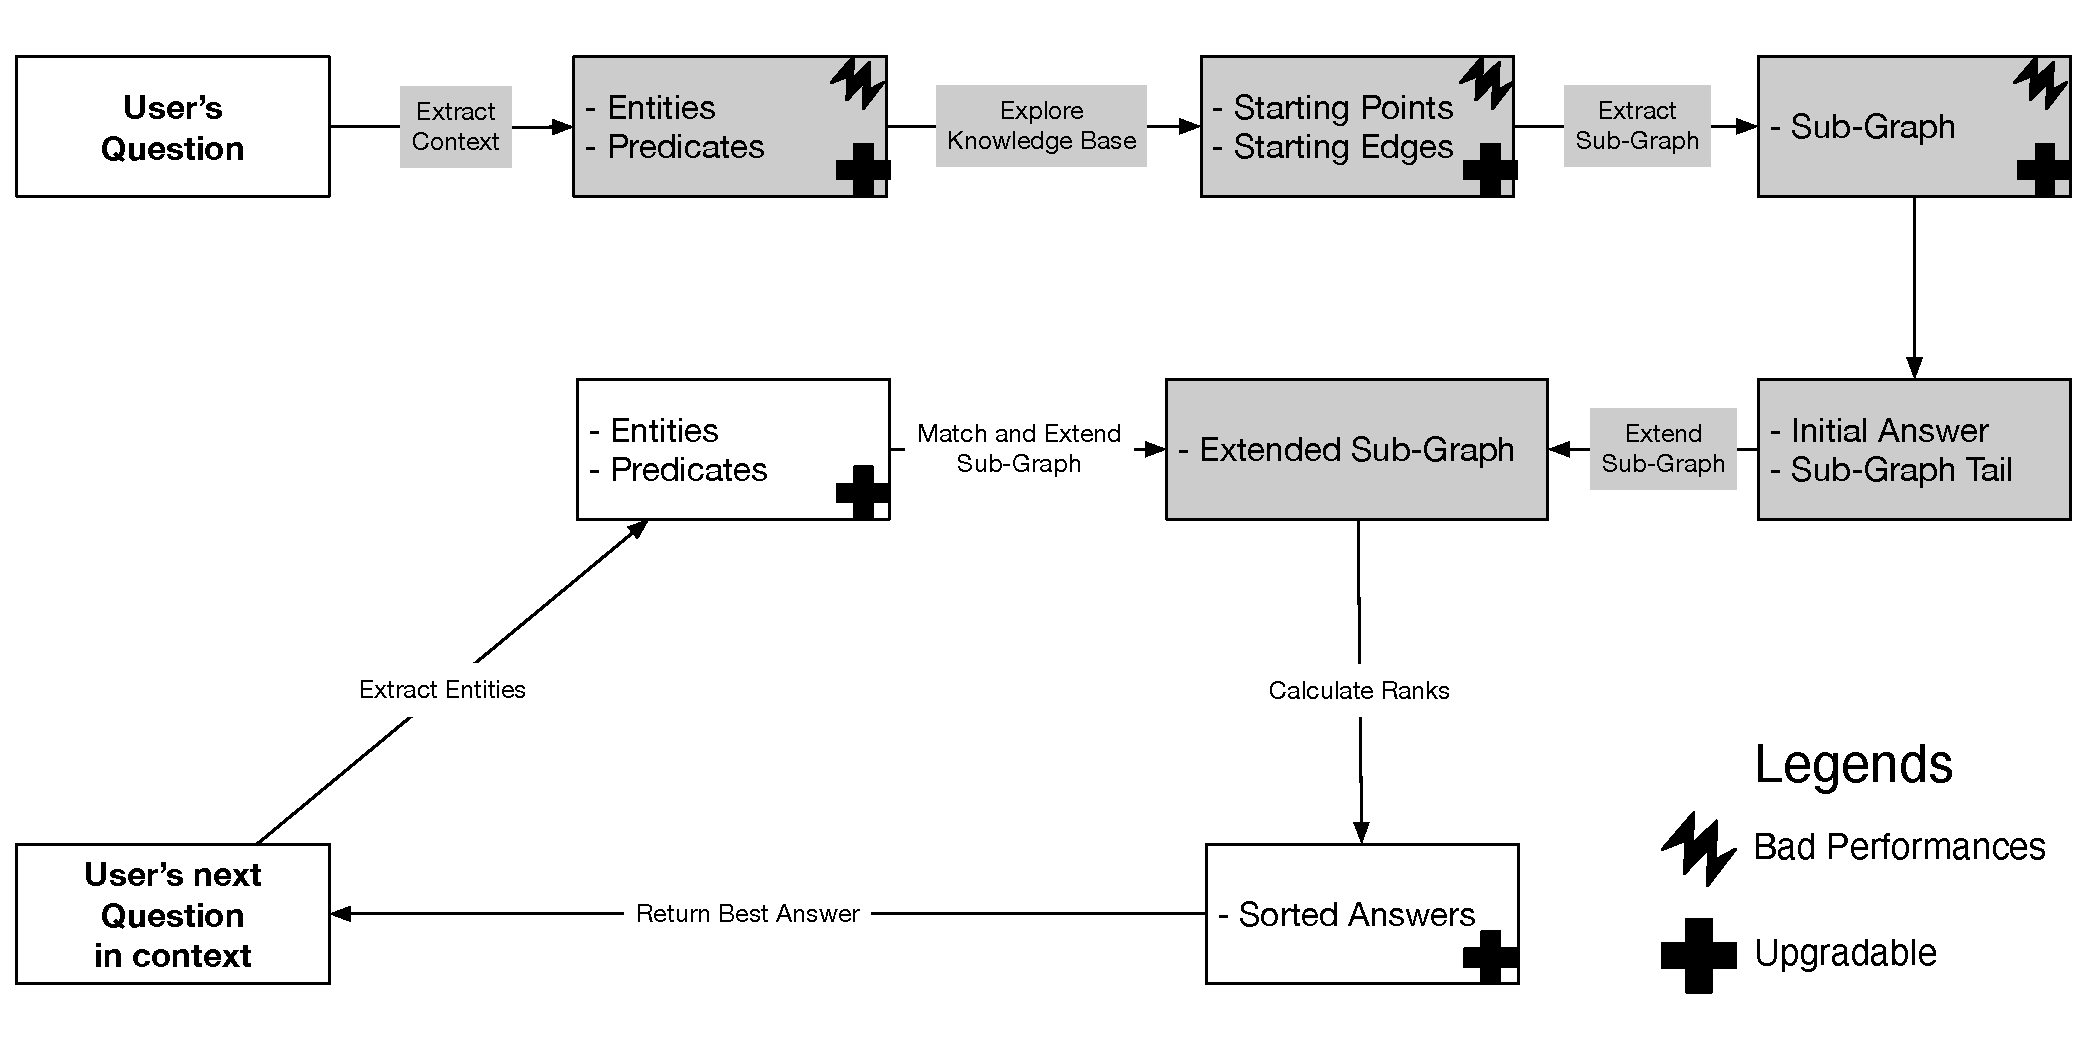
\includegraphics[width=\textwidth,keepaspectratio=true]{fig_high_level_convex_architecture_graphqa}
    \caption{Illustrative representation of the initial high level GraphQA architecture improving CONVEX. In grey, the architecture parts for GraphQA to rebuild.}
    \label{fig:fig_high_level_convex_architecture_graphqa}
\end{figure}



\subsection{Current Architecture}
Our architecture, as represented on Figure \ref{fig:fig_high_level_graphqa_architecture}, results from three major incrementations. It is, at first sight, heavier than the initial CONVEX-based architecture (see previous Section \ref{graphqa:initial}); however, its modular and generic design handles contextual graphs with an overall improvement toward the initial architecture as planned in the analysis. Indeed, as we built the project from the ground-up, we focused on the must-have features and pre-designed anchor points for the nice-to-have features as described in the final scope from our analysis (see chapter \ref{analysis:finalscope}). Additionally, as we aimed at a generic approach via modular orchestration, our \gls{qa} chatbot is by its architecture and design, extensible to further modules by either improve, replace or add new \gls{nlp} tasks.


\begin{figure}
    \centering
    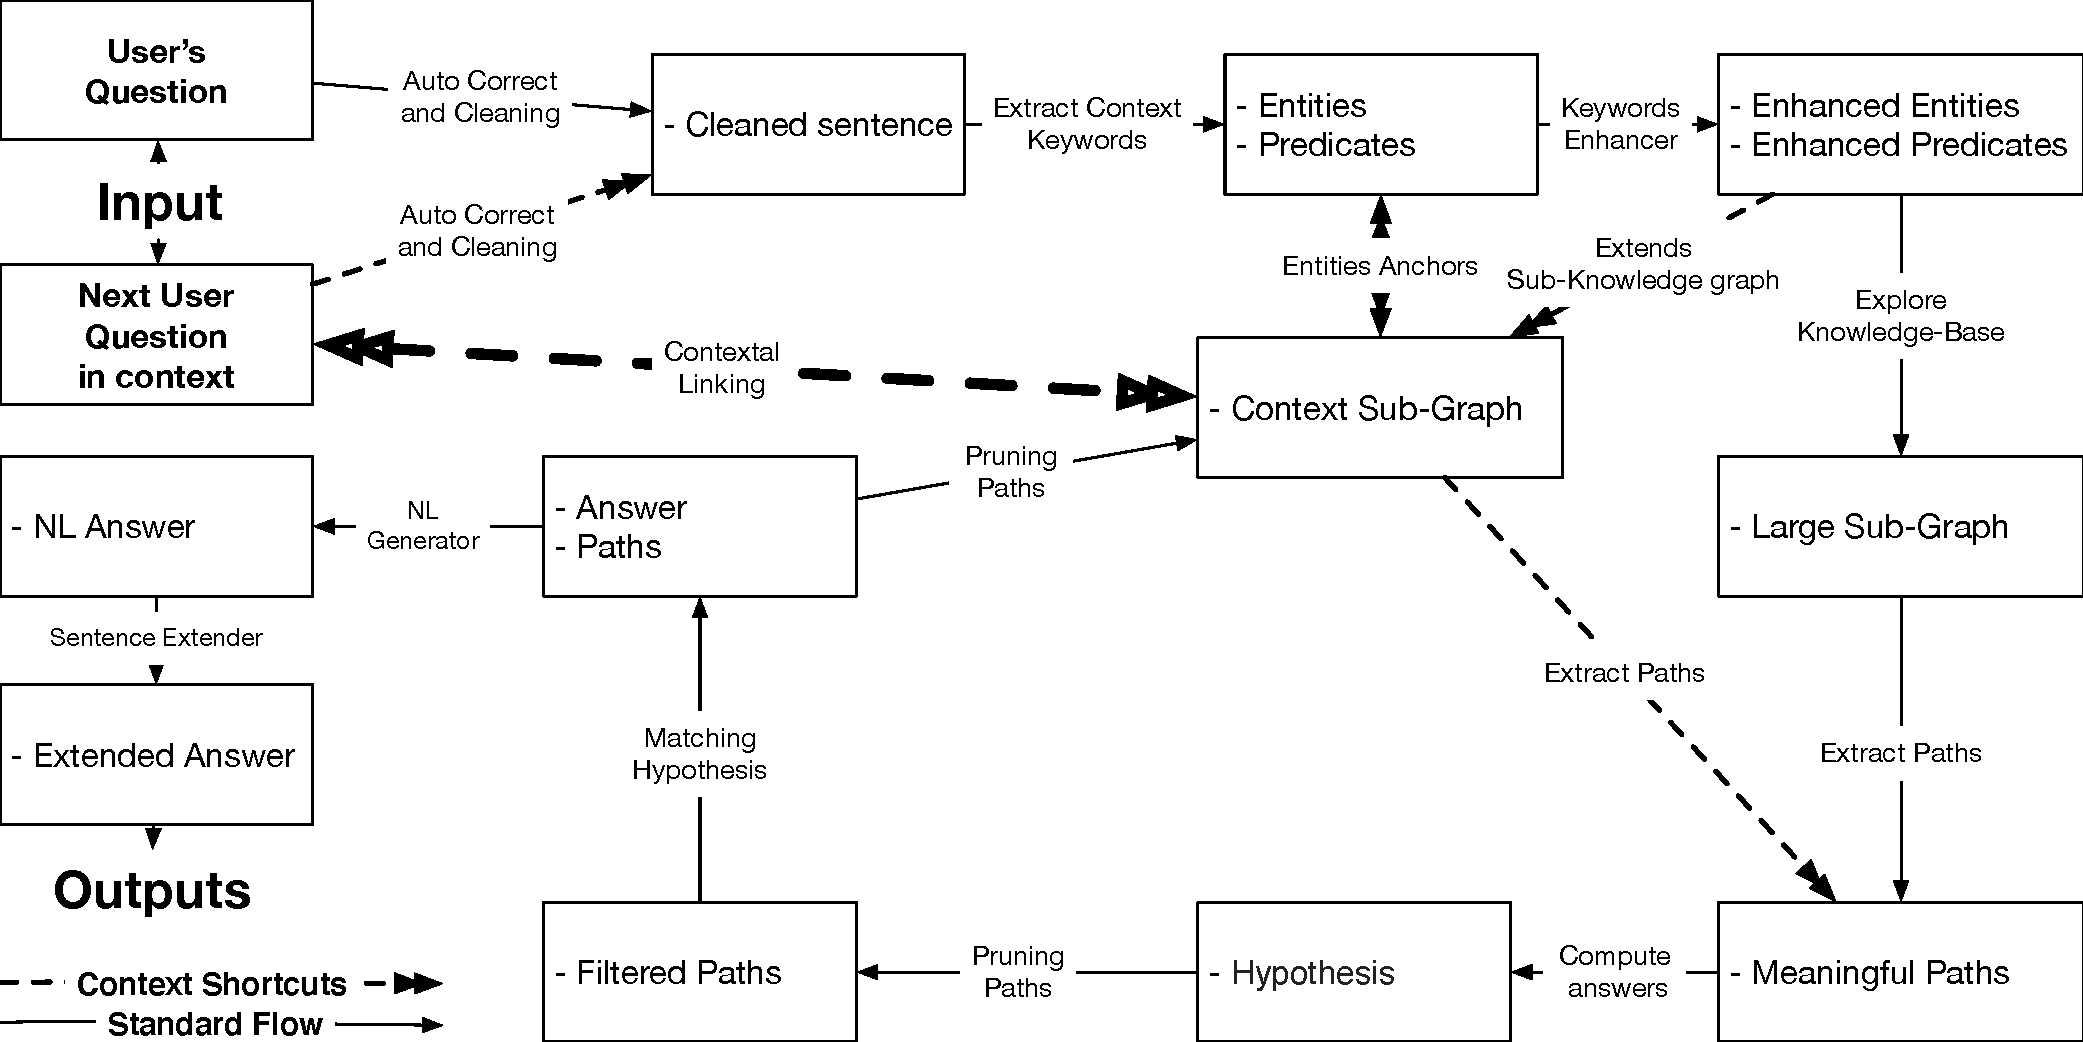
\includegraphics[width=\textwidth,keepaspectratio=true]{fig_high_level_graphqa_architecture}
    \caption{Illustrative representation of current high level GraphQA architecture. Double arrows indicates that the flow is related to context.}
    \label{fig:fig_high_level_graphqa_architecture}
\end{figure}

\subsection{Question Answering Pipeline}
In more details, we present on Figure \ref{fig:fig_graphqa_models_pipeline} our grounded tasks approach, implying a \gls{zero-shot} learning \gls{qa} system, as it doesn't not require any training examples to answer questions.

\begin{figure}
    \centering
    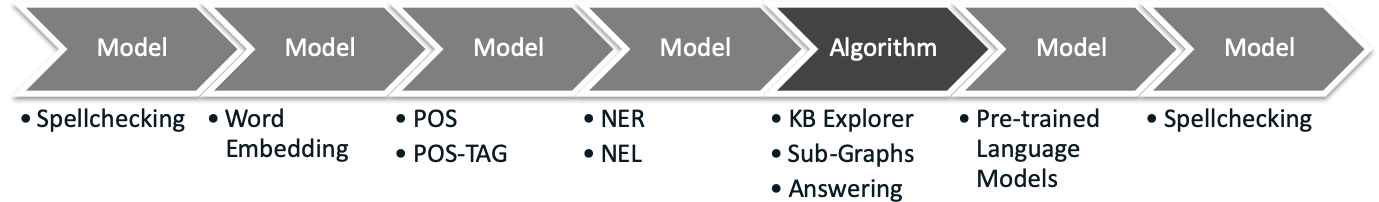
\includegraphics[width=\textwidth,keepaspectratio=true]{fig_graphqa_models_pipeline}
    \caption{Illustrative representation of GraphQA multi-models pipeline.}
    \label{fig:fig_graphqa_models_pipeline}
\end{figure}

\subsection{Dialogue Flow}
To illustrate in more details GraphQA Dialogue flow, Figure \ref{fig:fig_graphqa_dialogue_pipeline} presents our \gls{nl} answering approach for multi-turns conversations.

\begin{figure}
    \centering
    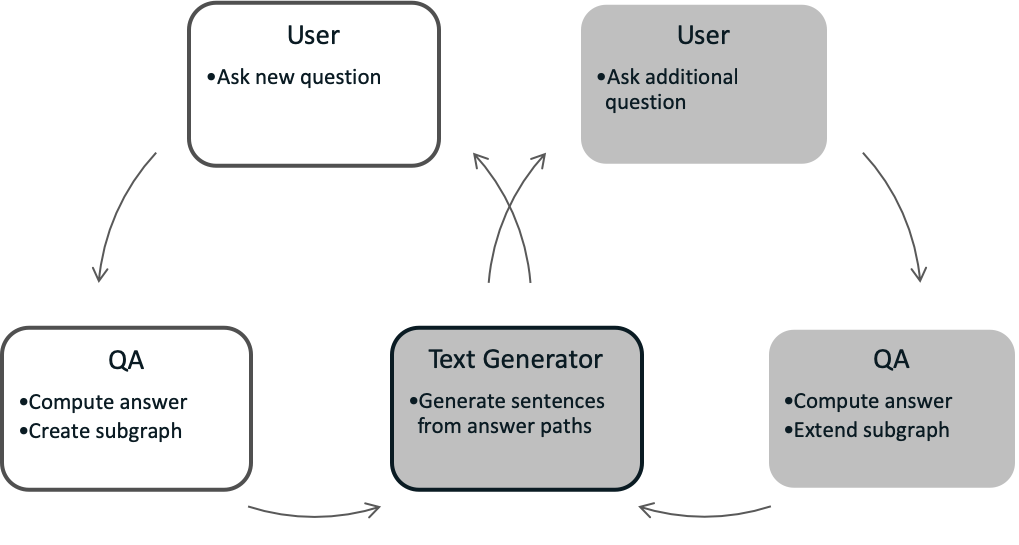
\includegraphics[width=\textwidth,keepaspectratio=true]{fig_graphqa_dialogue_pipeline}
    \caption{Illustrative representation of current GraphQA dialogue pipeline.}
    \label{fig:fig_graphqa_dialogue_pipeline}
\end{figure}

\section{Iteration 0}
The initial GraphQA version was CONVEX-based as we originally scoped to extend CONVEX features (see our previous sections \ref{graphqa:initial}). As we dove into the CONVEX implementation, we came across reproducibility issues and unexpected behaviors. After multiple contacts with the authors, we concluded that our interpretation of their paper was not as they intended to. Indeed, what we believed to be features, were from their point of view made-up feature for motivational purposes, which sadly deeply impacted our \gls{sota} analysis. However, during the initial phase, we understood the tools they built, giving us a head start for our architecture. Indeed, tools such as loading the \gls{wikidata} \gls{kb} and fetching \gls{spo} statements were reusable out-of-the-box. Optimizations such the HDT \autocite{website:hdt} and NetworkX \autocite{paper:SciPyProceedings_11} python libraries were a useful as starting points. 

\section{Major Iteration 1}
\label{graphqa:graphqa1}
Based on the toolset extracted version 0 from the CONVEX-based extender, GraphQA V1 is composed of the features listed below. During the iteration, we saw the opportunity to contribute to the \gls{nlp} field by building a recent version of the \gls{wikidata} \gls{kb} optimized HDT \autocite{website:hdt} format, as the latest dates from September 2018. Sadly, we were not able to generate an HDF dataset from the latest version of \gls{wikidata} \gls{kb} as we didn't have the required ram at our disposal to complete the task (about 240GB for 7.9 Million tuples).

\subsection{Library-based Features}
\label{graphqa:libraries1}
We are listing used libraries in the next section (see Section \ref{graphqa:techno}). Note that we may, in some cases, slightly enhance the basic library features, but we are keeping their main purpose intact.

\begin{itemize}
    \setlength\itemsep{0em}
    \item Retrieving statements from the \gls{wikidata} \gls{kb} via CONVEX
    \item \gls{nel} labels from the \gls{wikidata} \gls{kb} via CONVEX
    \item Document/Span/Word Embeddings via Spacy and GloVe
    \item Tokenization via Spacy
    \item \gls{pos} and \gls{pos-tag} via Spacy
    \item \gls{ner} for common word such as towns, countries, or famous people via Spacy
    \item Extract composed entities via Spacy
    \item Extract nested word groups within sentences via Spacy
    \item Build and explore sub-graphs via NetworkX
\end{itemize}

\subsection{Custom Features}
\label{graphqa:custom1}
The following features were designed with modularity in mind, as stated in the earlier sections. We describe them once here, but they are used in next versions. (See their algorithm subsections).

\subsubsection{Wikidata fine-tuned \gls{ner}}
Spacy's \gls{ner} is particularly impressive out-of-the-box; however, we found the need in the scope of the project to fine-tune Spacy's \gls{ner} model to help it identify Wikidata and Wikipedia pages names.

\subsubsection{Wikidata \gls{nel} training}
Spacy's provides training tools for additional models and includes them natively into its pipeline. We used the opportunity to build a \gls{nel} model linking our fine-tuned \gls{ner} model to also be able to linked the recognised pages to \gls{wikidata} \gls{kb} identifiers.

\subsubsection{Extract themes} 
The entities we call Themes are the most meaning words in a question; they define the initial anchor point to our \gls{qa} system. They have a stronger impact than keywords, as their purpose is to define the question in a meaningful manner.

To extract the question themes, we initially perform an entity check via Spacy's \gls{ner} on the sentence. 

To enhanced the \gls{ner} results, we extract nested word groups within sentences via Spacy's Document Embedding property \textbf{noun\_chunks}, then pass a \gls{ner} on the detected composites.

Additionally, we format the sentences into its Capitalised, Lowercased, Lemmatised, and Determinants-free forms, then apply Spacy's \textbf{noun\_chunks} property to altered sentences and pass a final \gls{ner} on the detected composites.

Note that the detected composites are the themes in our case.

\subsubsection{Enhance themes} 
During the theme extraction process, not all the words in the sentences are used as they have no meaning for our \gls{ner} model. In this module, we give a second chance to the trashed words by trying to match them to \gls{wikidata} entities by exploring the \gls{kb}.

To do so, we apply a similar technique than for theme extraction by formatting the word in their Capitalised, Lowercased, Lemmatised, and Determinants-free in its forms. We combine the words into multi-sized combination tuples then perform a lookup into the \gls{kb} to find a matching identity.

\subsubsection{Extract predicates} 
Often, questions are using inductive nouns or adjectives for predicates, making the naive approach of matching verbs to predicate not efficient. Our solution is to query the \gls{kb} with each word and evaluate the result as predicated. Additionally, we query \gls{wikidata} online with the specific type defining predicates, which often provides additional entities to our initial local query. Note that we initially built GraphQA intending to work in standalone without an internet connection, which makes the web querying sensible to our initial intention, but not against the project scope.

\subsubsection{Extract sentence focused parts} 
The module extracts word syntactically focused by the qualifier, such as who, where, or when. We use those words as initial answer anchors as, in most cases, is it possible to replace this word with the answer, and it converts the question into a descriptive sentence.

\subsubsection{Extract question keywords}
This module aims at capturing the relevant keywords from the question. It categorizes the keywords in three categories, the themes driven keywords, enhanced themes drive keywords, and predicates related to the focused parts. To do so, it uses similar techniques to the \gls{attention} by exploiting the extract word properties by Spacy's Document Embedding model, and the entities present in the sub-knowledge graph.

\subsubsection{Extract keyword related paths}
Based on dynamic thresholds, this module uses previously extracted keywords to extract paths from the raw sub-knowledge graph.

\subsubsection{Filter extracted paths}
The module parses the extract keyword paths to fix malformed \gls{spo} chains by extending further the path and finishes by removing duplicates and sublists.

\subsubsection{Compute answer hypothesizes}
The process consists of rebuilding the question in its descriptive form with \gls{spo} extractions from each filtered path. The final score combines the computed score for each word with an overall rating for each path. The scores are defined either with positive or negative values depending on the evaluated tasks such are word proximities.

\subsubsection{Build the sub-knowledge graph}
Based on the extracted themes, enhanced themes, and predicates, this module explores the \gls{wikidata} \gls{kb} for statements, uses the extracted themes as subject and extracted predicates as predicates and adds matching statements into an empty NetworkX graph.


\subsection{Algorithm}
Here is enumerated the overall process to compute the answer from a question.

\begin{enumerate}
    \setlength\itemsep{0em}
    \item Builds a Document Embedding of the question
    \item Extracts the themes
    \item Extracts the enhanced themes
    \item Extracts the predicates
    \item Extracts the question focused parts
    \item Builds a sub-knowledge graph
    \item Rebuilds the graphs with a higher deepness if it contains too many elements
    \item Extracts the question keywords
    \item Extracts the question-related paths from the sub-knowledge
    \item Filters the extracted paths
    \item Computes and sort hypothesizes
    \item Extracts the paths containing the best hypothesis as the first or last element
\end{enumerate}

\subsection{Major Iteration 2}
\label{graphqa:graphqa2}
In addition to some computational parallelization, tweaks, and optimizations, the second version of GraphQA aims to provide a wiser answer by not trusting the initial best hypothesis score but instead considering all the hypotheses by additionally scoring the matching for each hypothesis within the question itself. We added global banned entities such as linking ids to other \gls{kb}. Finally, the algorithm can handle various computational decisions via predefined thresholds dynamically.

\subsection{Library-based Features}
\label{graphqa:libraries2}
We hereby list only the additional features to the first version (see subsection \ref{graphqa:libraries1}). See Section \ref{graphqa:techno} for the libraries listing.

\begin{itemize}
    \setlength\itemsep{0em}
    \item Auto correcting the questions from the user via DeepCorrect
    \item Replacing recognised names from Wikipedia \gls{ner} within the question via DeepCorrect
\end{itemize}

\subsection{Custom Features}
We hereby list additional and modified features to the first version (see subsection \ref{graphqa:custom1})

\subsubsection{Compute answer hypothesizes by handling types}
The second iteration of this module uses word embedding similarities for its scoring tasks; additionally, it now has the notions of Locations, Persons, Dates, Causes, Quantities, and Selective questions to refine the scoring to the answer types. Finally, we enhanced the scoring formula to handle the overall path score while computing the individual \gls{spo} scores.

\subsubsection{Evaluate hypothesizes}
This module calculates a score for each hypothesis by replacing the hypothesis with the focus part within the question and comparing the new descriptive sentence to the original question. Additionally, it explores the \gls{kb} to reconstruct the original path by giving a higher weight to qualifiers, and gives a score based on the success of the task.

\subsubsection{Answer paths extractor}
Use the fact that we can trust the hypothesizes evaluator to return the best-fitting answer to the question, we enhanced the answer path extractor also to include paths where the answer is not in the first of the last place.

\subsection{Algorithm}
Here is enumerated the overall process to compute the answer from a question. In bold are highlighted the new tasks.

\begin{enumerate}
    \setlength\itemsep{0em}
    \item \textbf{Removes unsupported characters from the question}
    \item \textbf{Autocorrects the question and replaces with Wikipedia names via \gls{ner}}
    \item Builds a Document Embedding of the question
    \item Extracts the themes
    \item Extracts the enhanced themes
    \item Extracts the predicates
    \item Extracts the question focused parts
    \item Builds a sub-knowledge graph
    \item Rebuilds the graphs with a higher deepness if it contains too many elements
    \item \textbf{Rebuilds the graphs with a lower deepness if it does not contain a minimum of elements}
    \item Extracts the question keywords
    \item Extracts the question-related paths from the sub-knowledge
    \item Filters the extracted paths
    \item Computes and sorts hypothesizes
    \item \textbf{Evaluates and sorts the hypothesizes}
    \item \textbf{Extracts the paths containing the best hypothesis}
\end{enumerate}


\section{Major Iteration 3}
\label{graphqa:graphqa3}
In addition to now handle multi-turns conversations within a context sub-graph, GraphQA is completely parallelized, which improves the overall answering speed by 50\%, but does not solve the speed impact of computation (see the results Chapter \ref{chap:results}). Numerous tweaks have taken place and made the overall answering better compared to the previous iteration. Finally, GraphQA in the current state returns answers in \gls{nl}, with the option to extend them with \gls{kb} and random facts.

\subsection{Library-based Features}
We hereby list only the additional features to the second version (see subsection \ref{graphqa:libraries2}). See Section \ref{graphqa:techno} for the libraries listing.

\begin{itemize}
    \setlength\itemsep{0em}
    \item Use of BERT-large pre-trained language model via Huggingface
    \item Use of GPT-2-XL pre-trained generative language model via Huggingface
\end{itemize}

\subsection{Custom Features}
We hereby list additional and modified features to the first version (see subsection \ref{graphqa:custom1})

\subsection{Sub-Knowledge Graph optimnizations}
We enhanced the initial sub-knowledge graph extractor by additionally filtering clusters and removing clusters unrelated to the questions.

\subsection{Binary answers}
This module handles binary questions by exploring the sub-knowledge graph to detect the presence of the focused part.

\subsubsection{Context holding in sub-graphs}
We prune the sub-knowledge graph from clusters entities to the computed answer. We call the pruned sub-knowledge graph Context Graphs, as they only hold the context to the question and previous answer.

\subsubsection{Multi-turn conversations}
In addition to handling context graphs during \gls{qa}, by using the entities already present in the context graph to drive the \gls{kb} exploration and replace pronouns in the new question, the module keeps track of the previous direct questions and weights the keywords to it.

\subsection{\gls{nl} answers}
Until the second version, we returned the fact answer and the best paths from the answer. This module uses the masking feature from \gls{bert} \autocite{paper:devlin-etal-2019-bert} to fill the gaps between \gls{spo} within the answering paths.

\subsection{Context facts extender}
By default, the \gls{nl} answers computes the returned \gls{spo} based on the question, but it is also possible to manually increase the amount of \gls{spo} to return, which increase the original \gls{nl} answers to additional facts extracted from matched paths.

\subsection{Random facts extender}
For gamification purposes, it is also possible to extend the \gls{nl} answers with generated random facts using \gls{gpt2}.

\subsection{Handling Pre-built graph}
GraphQA can be plugged to any \gls{qa} system, as it only requires a context graph, which can hold from none to any amount of nodes and edges, and optionally keywords from the previous conversation. This feature makes it a nice candidate to give the ability to non-conversational \gls{qa} systems to handle Multi-turn conversations.

\subsection{Algorithm}
Here is enumerated the overall process to compute the answer from a question. In bold are highlighted the new tasks.

\begin{enumerate}
    \setlength\itemsep{0em}
    \item Filters the sentence from unsupported characters
    \item Autocorrects the question and replaces with Wikipedia names via \gls{ner}
    \item \textbf{Handles previous context}
    \item Builds a Document Embedding of the question
    \item Extracts the themes
    \item Extracts the enhanced themes
    \item Extracts the predicates
    \item Extracts the question focused parts
    \item \textbf{Extends previous context graph}
    \item Builds a sub-knowledge graph
    \item Rebuilds the graphs with a higher deepness if it contains too many elements
    \item Rebuilds the graphs with a lower deepness if it does not contain a minimum of elements
    \item \textbf{Answers binary questions based on the graph}
    \item Extracts the question keywords
    \item Extracts the question-related paths from the sub-knowledge
    \item Filters the extracted paths
    \item Computes and sorts hypothesizes
    \item Evaluates and sorts the hypothesizes
    \item Extracts the paths containing the best hypothesis as the first element
    \item \textbf{Extracts context graph from sub-knowledge graph}
    \item \textbf{Builds a \gls{nl} answer}
    \item \textbf{Extends the \gls{nl} answer with context graph}
    \item \textbf{Extends the \gls{nl} answer with random facts}
\end{enumerate}


\section{Technologies}
\label{graphqa:techno}
The following are the technologies used by GraphQA.

\paragraph{HDT}
\autocite{website:hdt} It is a query compression format for linked data; it compresses the RDF database and loads its index into the RAM for querying. 

\paragraph{Spacy}
\autocite{paper:spacy2} It is an impressive framework used in the industry for its multiples \gls{nlp} tools, pre-builts models and easy to use fine-tuning pipelines. It allows handles Document Embedding, \gls{we} via GloVe \autocite{paper:glove}, \gls{ner} \gls{nel}, \gls{pos}, \gls{pos-tag}, Tokenization, and much more. On a side note, we used the version 2 released in 2019. 

\paragraph{DeepCorrect}
\autocite{website:deepcorrect-github} It is a project exploring the \gls{dl} for text and punctuation correction with a pre-trained model on Wikipedia.

\paragraph{NetworkX}
\autocite{paper:SciPyProceedings_11} It is a Python package used for the creation and manipulation of graphs.

\paragraph{Huggingface}
\autocite{paper:2019arXiv191003771W} It is a startup focusing on \gls{nlp} tools, in particular \glspl{transformer}. They provide frameworks to use pre-trained language model out-of-the-box, making them popular in the \gls{nlp} field and the industry.

\section{Dev Benchmarking Questions}
For each GraphQA version, we used the same six development questions to evaluate our work superficially. Additionally, we incrementally increased a pool of questions triggering error while performing benchmarks on the SimpleQuestions and ConvQuestions datasets, which we kept as debugging purposes and tracker for the consistency across our incremental versions.

\subsection{Single-hop Questions}
Here is our two development \gls{sh} questions.
\begin{itemize}
    \setlength\itemsep{0em}
    \item \say{Who is the wife of Barack Obama?}
    \item \say{of what nationality is ken mcgoogan}
\end{itemize}
    

\subsection{Multi-hop Questions}
Following is our two development \gls{mh} questions.
\begin{itemize}
    \setlength\itemsep{0em}
    \item \say{What is the name of the writer of The Secret Garden?}
    \item \say{Which actor voiced the Unicorn in The Last Unicorn?}
\end{itemize}

\subsection{Multi-hop and Multi-Turns Questions}
Following our two development \gls{mh} and multi-turn questions.
\subsubsection{Conversation 1}
\begin{enumerate}
    \setlength\itemsep{0em}
    \item \say{Which actor voiced the Unicorn in The Last Unicorn?}
    \item \say{And Alan Arkin was behind..}
    \item \say{Who did the score?}
    \item \say{So who performed the songs?}
    \item \say{Genre of this band}
    \item \say{By the way, who was the director?}
\end{enumerate}

\subsubsection{Conversation 2}
\begin{enumerate}
    \setlength\itemsep{0em}
    \item \say{Who is the author of the Harry Potter series?}
    \item \say{What was the year of publication for the first book?}
    \item \say{The first book was called what?}
    \item \say{It was set in what country?}
    \item \say{Which book has the highest page count?}
\end{enumerate}


\section{Further Exploration Ideas}
This section provides a non-exhausting list of exploratory ideas for future related studies.

\begin{itemize}
    \setlength\itemsep{0em}
    \item Use a pre-trained language model such as \gls{bert} as word embedding instead of GloVe.
    \item Fine-tune a pretrain language model such as \gls{bert} for \gls{nel}.
    \item Fine-tune a pretrain language model such as \gls{bert} to add a multi-brains approach as slightly mentioned in the analysis \ref{chap:analysis} brainstorming. Where multiple models are answering simultaneously the same question, and reach a consensus for the final answer.
    \item Query \gls{wikidata} online for cross-checking local entities and enhanced themes.
    \item Prebuild context graph for contents such as Articles to increase speed and target the information.
    \item Context graph bridging multiple prebuilt graphs to gather information faster and long-distance context handling
    \item Extend context graphs for user experience personalization by keeping long-term contexts.
\end{itemize}


\section{Interesting Facts}
On a final note, we also wanted to mention a non-exhausting list of problems that occurred during the making of GraphQA that we believe are interesting facts.

\begin{itemize}
    \setlength\itemsep{0em}
    \item The uncompressed version of the latest \gls{wikidata} dump is 500 GB.
    \item Knowledge Bases do not have the same conventions for Subject-Predicate-Object Tuples (SPOs).
    \item Nested Tensorflow sessions are not working as expected when called.
\end{itemize}



%\chapter{Conclusions}
\label{chap:dev-conclusions}
\cleardoublepage

% PART 4
\part{Retrospective}
\chapter{Results}
\label{chap:results}
\chapter{Discussion}
\label{chap:discussion}

The following chapter summarizes our state of mind about the project. As we choose a storytelling approach for our Master's Thesis, discussions were diluted within all chapters making the traditional academic discussion chapter, the only place to discuss our humble opinions. First of all, we want to remind that GraphQA is a \gls{poc}, and its performances are not particularly important, as it is the project itself, with its original approaches that must be evaluated. As an observation, we are using \gls{sota} technologies mostly released in late 2019 (and even for some, such as CONVEX was released during our last \gls{sota} sprint), reinforcing our statement that \gls{nlp} is driving a lot of interest lately. To structure this chapter, we will mostly talk about our main competitor and its dataset. Indeed, we indirectly spent the Master's Thesis analyzing their work, as GraphQA is using a similar sub-knowledge graph approach. We believed that it is important to discuss how our competitors perform. We will finally overview what we learned from our overall research and threw a few questions that are left to answer.


\section{ConvQuestions Dataset}
As we praised this dataset the whole thesis, we believe for good reason, as it a \gls{sota} in the field of  \gls{mh} and multi-turns. However, in this section we will overview the dataset their contribution to \gls{nlp}, the limitation, and the required improvement for future \gls{mh} and multi-turns conversational datasets.

\subsection{Data Augmentation}
As a contribution, ConvQuestion, they suggested a new data augmentation approach for \gls{nlp}. Data augmentation is very popular in the field of Computer Vision; however, it is often a bad solution in \gls{nlp} as it often uses computer-generated paraphrasing by applying \gls{we} similarities. With ConvQuestion, the authors took a clever shift by asking humans to generate the paraphrasing, with the constraint that the paraphrased sentence must be semantically equivalent and interchangeable with its original sentence. Besides, ConvQuestions guarantees that the conversations are not permuted to not alter nested questions. It won't surprise us that \gls{qa} evaluation-based datasets such as \gls{squad} will use this method to enhance their datasets. On a final note, ConvQuestions is a relatively small dataset with its 11'200 questions compared to the 150'000 questions from \gls{squad} 2.0; however, the plot twist is that ConvQuestion used a total of 1'750 unique questions to generate their dataset with only a single permutation per questions.

\subsubsection{Paraphrasing examples}
\textbf{Who is the author of the Harry Potter series?} Who wrote Harry Potter?\\
\textbf{What was the year of publication for the first book?} When was it first published?\\
\textbf{Title of the first book?} The first book was called what?\\
\textbf{What country was the book set in?} It was set in what country?\\
\textbf{Which book has the highest page count?} What's the longest book?

\subsection{Human Errors}
\label{discussion:humans}
The main limitation we noticed is the crowdsourcing itself. Even if this solution is at the time of writing, probably the best to generate \gls{nlp} datasets, Mechanical Truckers often make mistakes. Indeed, it is difficult for large datasets to have no mistakes; it is human nature to get distracted, particularly for repetitive tasks such as being a Mechanical Trucker. A common inattentiveness we noticed, in addition to laziness while paraphrasing (see the previous subsection), is that the truckers do answering mistakes and are not always respecting the format guidelines, implying 32 ($2^5$) wrong question-answers tuples for a single mistake. For a small dataset such as ConvQuestion, the ratio of unanswerable tuples can rise dramatically and induce important bias while training models. We regret that the author didn't take the time to review correctly their relatively small dataset, or implement a crowdsourced cross-checking protocol like \textit{Google} did for their Natural Dialogue dataset \autocite{paper:google-natural-questions}. 

\subsubsection{Mechanical Trucker error examples}

\paragraph{Answering Mistake}
In this situation, the Trucker provided the wrong answer to the question. \\
\textbf{Question:} When did the first The Fast and the Furious film come out?\\
\textbf{Expected answer:} 1955\\
\textbf{Wrong answer:} 22 June 2001


\paragraph{Inattentiveness} 
For this example we extrapolate the expected answer from the full \gls{nl} answer span \say{The first film came out 22 June 2001.}. \\
\textbf{Question:} When did the first The Fast and the Furious film come out? \\
\textbf{Expected answer:} 22 June 2001 \\
\textbf{Trucker's answer:} https://www.wikidata.org/wiki/Q155476\\

\paragraph{Not Respecting the Answer Guideline} 
In this example, the Trucker did not providing a \gls{nl} answer span. \\
\textbf{Question:} When was he born? \\
\textbf{Answer:} 1 August 1819 \\
\textbf{Answer Span:} 1 August 1819 \\


\subsection{GraphQA}
The previous sections would probably not exist if GraphQA didn't find them. Indeed, as we were monitoring GraphQA answers, we noticed that sometimes the answers were correct, but the benchmark said otherwise. To our regrets, due to time constraints, we could not go through the whole dataset; however, this observation implies that an application for GraphQA and its competitors could be to \gls{oracle} crowdsourced datasets.


\section{CONVEX}
In our opinion, CONVEX is a pioneer in the field of sub-knowledge graphs and we amire their approach as they inspired  GraphQA. They were chosen during our analysis as a starting project for our \gls{qa} system and planned to enhance their work. However, as stated in the GraphQA chapter \ref{chap:graphqa}, we took another path and, in the following sections, we want to discuss this decision and discuss their work as our main competitor.

\subsubsection{Initial Issues}
Our initial grip with CONVEX code was not the smoothest, as the authors provided their code in the state with few refactoring bugs. We contacted the authors and debugged the code together; then, we decided to fork the project and continue on our own by fixing and adapting the code to our needs as GraphQA progressed. After the project investigation, we noticed that we could not reproduce the results in the paper. We contacted the authors to notify the issues: they explained that they used an undisclosed split of the dataset to obtain their results, and confirmed that the code works as expected.

\subsubsection{Q0 Problems in more details}
Based on the previous authors' statement, we started to investigate further how CONVEX answers questions. As the paper acknowledges that Q0 is their bottleneck, we decided to explore further why it is indeed a bottleneck; we observed that often the answers are lucky guesses as it returns the first Object from a multi solutions Subject-Predicate tuples. E.g., \say{Who is the actor of this role in this movie?}: by design, the query would return the list of all actors to the requested movie, which we call hypothesis in GraphQA. CONVEX, in this particular case, will return the first element. Their \gls{ner} depends on TAGME, which is proprietary, meaning that it's up to a black box to return the \gls{wikidata} entity identified based on the context of the sentence. It is indeed hard to trust a proprietary system to return the right entities when multiple entities have the same name.

\subsubsection{GraphQA from Scratch}
Based on the previous analysis, it was clear that building an open-source module for Q0 was the priority task. We investigated in details how to integrate our module to the existing system, by going deeper into the code and understanding all functions. Aside from odd computations, we could not find the context-graph generation as described in the paper, so we asked the author about it. They explained that the part we are looking for, which we imagined to be the most exciting, were written in the paper with made-up values for motivational purposes. From this point, we lost all motivation to enhance CONVEX as its key feature was not implemented and required an architecture remodeling to get it to work. Annoyingly, the clock was ticking, and we could not step back to evaluate a new solution. Based on the CONVEX's motivational purpose feature, we built from scratch an open-source architecture handling scoring by design. (See chapter \ref{chap:graphqa})


\section{Lesson Learned}
This project gave us lessons about the academic experience and the field of \gls{nlp}.

\subsection{Only trust yourself}
\paragraph{Preprints} Some papers are good, but they are mostly bad as they are either repetitive or pointless with name-dropping.
\paragraph{Published in journal} Mostly good, they often do nested research by publishing a paper at each iteration of their project.
\paragraph{Published in conferences} Often useful, but be careful with the origin country.
\paragraph{Repetitivity} We realized that after a reasonable amount of paper read, we are not surprised anymore about the breakthroughs.
\paragraph{Never trust claims in articles} Always reproduce the results and inspect the given code and datasets.
\paragraph{Stay critic} Every day a new \gls{sota} or baseline is claimed, wait for reproduced results before excitement.

\subsection{Don't trust Mechanical Trucks}
As stated in the previous section \ref{discussion:humans}, it is essential when using Mechanical Trucks always to add a verification layer.


\section{Questions Left}
As our project end, in addition to questioning seeds left in chapters, we still have remaining questions that we wished we had time to explore. We listed them here as a starting point for GraphQA enhancement or other contributions.

\begin{itemize}
    \setlength\itemsep{0em}
    \item Would it be possible for \gls{qa} system to become sophist, and what would be the implications?
    \item Would it be possible to use GraphQA as a sophist chatbot?
    \item Would it be possible to train a model to use context graphs?
    \item Would it be possible to build a tool for users to create context graphs manually?
    \item Would it be possible to build a tool to parse articles and generate context graphs automatically? 
    \item Investigate the correlation between human thinking and reasoning with knowledge graphs representation.
    \item Compare knowledge graphs representation to \gls{ir} and access structure.
    \item Compare Wordnet and \gls{we} in the scope of GraphQA.
\end{itemize}













\chapter{Project Management}
\label{chap:final-project-management}

\todo{The milestones were meant to be adjustable based on how the project go}

To avoid getting overwhelmed with the latest \gls{nlp} papers in the field of \gls{qa} systems, and \glspl{gs}, the author defined workflow components to gather valuable information:

\begin{itemize}
    \setlength\itemsep{0em}
    \item Get up to date with the \gls{nlp} technologies used at \textit{iCoSys}.
    \item Explore community-made curated lists\footnote{Using \textit{Awesome} lists from \url{github.com} as starting point}.
    \item Stay informed of the breakthroughs via social medias\footnote{Examples from \url{reddit.com} /r/MachineLearning, /r/LanguageTechnology, /r/deeplearning}.
    \item Find reviews and articles vulgarizating recent papers\footnote{Particularly from community based \url{medium.com} articles}.
    \item Read papers\footnote{Most of the articles are coming from \url{arxiv.com} and \url{aclweb.org}}.
\end{itemize}

\section{Objectives}
\subsection{Intrinsic}
This subsection presents the general objectives related to the master's thesis.
\paragraph{Primaries}
\begin{itemize}[noitemsep]
    \item Propose a project specification and planning.
    \item Analyze the state of the art of existing technologies and technics of \gls{qa} systems and \gls{generative} \gls{ai}.
    \item Overview digital transformation in journalism and review the current status of the AI-News project.
    \item Document the study and write the thesis.
\end{itemize}

\subsection{Fact-based \acrlong{qa} Chatbot}
The first objective is to make, based on the \glsfirst{sota}, an algorithm that takes a question as input and outputs a response, as illustrated on Figure~\ref{fig:intro_qa}
\begin{figure}[ht!]
    \centering
    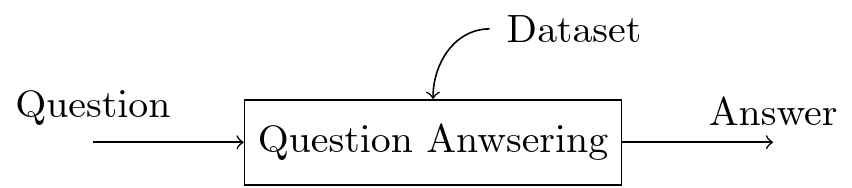
\includegraphics[width=\textwidth,height=2.1cm,keepaspectratio=true]{intro_qa}
    \caption{Suggested \gls{qa} diagram}
    \label{fig:intro_qa}
\end{figure}

\paragraph{Primaries}
\begin{itemize}[noitemsep]
    \item Select existing papers and projects treating the subject as a starting point.
    \item Identify relevant datasets.
    \item Develop one or more \gls{poc}.
    \item Test and evaluate solutions.
    \item Suggest improvements, possible continuation, and future outcomes.
\end{itemize}
\paragraph{Secondaries}
\begin{itemize}[noitemsep]
    \item Extend the \gls{qa} chatbot using "tailored" knowledge, e.g., \gls{model-ft} with press content.
\end{itemize}

\subsection{\gls{generative} \gls{qa} Chatbot}
The second objective is to extend the output from the \gls{qa} system, from the first objective, by enhancing the answers and generate human-like sentences from the enhanced answers. The initial vision for this objective is as illustrated in Figure~\ref{fig:intro_qa_gen}, a two parts system. The \textit{Enricher} enriches the answer from the \gls{qa} system, e.g. using a knowledge base\footnote{Wikidata.org, a Freebase-based  \autocite{paper:bollacker2008} knowledge base or Google's Knowledge Graphs \autocite{blog:intro_knowledge_graph}}. The \textit{Generator} aims at creating readable text from the enriched answer. Besides, we could also use user profiles\footnote{Fictive profiles in the context of the thesis} as input to those two parts.
\begin{figure}[ht!]
    \centering
    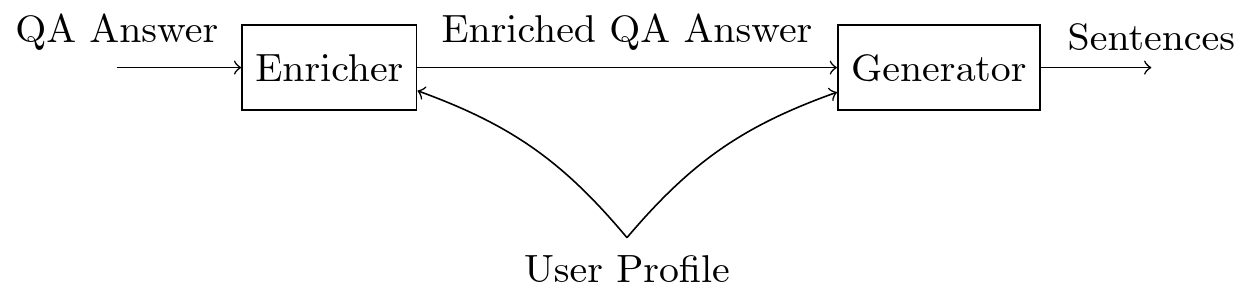
\includegraphics[width=\textwidth,keepaspectratio=true]{intro_qa_gen}
    \caption{Suggested \gls{generative} \gls{qa} diagram}
    \label{fig:intro_qa_gen}
\end{figure}


\paragraph{Primaries}
\begin{itemize}[noitemsep]
    \item Investigate a rule-based system for keyword enrichment.
    \item Generate sentences with keywords.
    \item Identify relevant datasets.
    \item Develop one or more \gls{poc}.
    \item Test and evaluate solutions.
    \item Suggest improvements, possible continuation, and future outcomes.
\end{itemize}
\paragraph{Secondaries}
\begin{itemize}[noitemsep]
    \item Use advanced strategies to enrich keywords.
    \item Use advanced text generation technics such as GTP-2\footnote{OpenAI's GTP-2 Algorithm \autocite{papers:gpt2}}.
    \item Use user profiles to customize the outputs.
\end{itemize}


\section{Initial Plan}
\label{plan:plan}
\subsection{Contraints}
\textbf{Timeframe:} 19 weeks\\
\textbf{Starting date:} 16.09.2019\\
\textbf{Ending date:} 07.02.2020

\subsection{Methodologies}
For consistency, the project is separated into two methodological parts. The first third, as the project targets information gathering and self-study, we use a standard sequential project management methodology. For the next two-thirds of the project, we will be using an agile methodology to perform incremental progress while exploring.

\subsubsection{Back to level Milestones}
First third of the study, from \textbf{16.09.19 to 25.10.19 (6 weeks)}.
\begin{enumerate}
    \setlength\itemsep{0em}
    \item[M1.] Initial \gls{mt} plan and project specification
    \item[M2.] Review the state of the art of the \gls{nlp} and \gls{nlu} technologies and refine the plan if needed.
\end{enumerate}


\subsubsection{Diving into the subject Milestones}
\textbf{From 28.10.19 to 07.02.20 (13 weeks)}, the following two-third of the work is composed of 6 sprints of two weeks each and one week to finalize the thesis.
\begin{itemize}
    \setlength\itemsep{0em}
    \item[M3.] Basic \gls{qa} Chatbot
    \item[M4.] Evaluation of basic \gls{qa} Chatbot
    \item[M5.] Basic generative \gls{qa} Chatbot
    \item[M6.] Evaluation of basic generative \gls{qa} Chatbot
\end{itemize}

\subsection{Gantt}
The Figure~\ref{fig:gantt-initial} represents the chart for the initial plan.

\newganttchartelement*{project-milestone}{
project-milestone/.style={
shape=isosceles triangle,
inner sep=0pt,
draw=cyan,
top color=white,
bottom color=cyan!50
},
project-milestone incomplete/.style={
/pgfgantt/project-milestone,
draw=yellow,
bottom color=yellow!50
},
project-milestone label font=\slshape,
project-milestone left shift=0pt,
project-milestone right shift=0pt
}

\newgantttimeslotformat{stardate}{
\def\decomposestardate##1.##2\relax{
\def\stardateyear{##1}\def\stardateday{##2}
}
\decomposestardate#1\relax
\pgfcalendardatetojulian{\stardateyear-01-01}{#2}
\advance#2 by-1\relax
\advance#2 by\stardateday\relax
}

\begin{figure}[h]%[htbp]
\centering
\begin{ganttchart}[vgrid, hgrid]{1}{19}
\gantttitle{Sep}{2} 
\gantttitle{Oct}{5}
\gantttitle{Nov}{4}
\gantttitle{Dec}{3}
\gantttitle{Jan}{4}
\gantttitle{Feb}{1}\\
\gantttitlelist{1,...,19}{1}\\

%part 1
\ganttgroup{Back to level}{1}{6} \\
\ganttmilestone{M1, M2}{3}
\ganttmilestone{}{6}\\

%part 2
\ganttgroup{Diving}{7}{18} \\
\ganttbar{Sprint 1}{7}{8} \\
\ganttbar{Sprint 2}{9}{10} \\
\ganttmilestone{M3}{10}\\
\ganttbar{Sprint 3}{11}{12} \\
\ganttmilestone{M4}{12}\\
\ganttbar{Sprint 4}{13}{14} \\
\ganttbar{Sprint 5}{15}{16} \\
\ganttmilestone{M5}{16}\\
\ganttbar{Sprint 6}{17}{18} \\
\ganttmilestone{M6}{18}\\

%\ganttlink{elem6}{elem7}
%\ganttlink{elem8}{elem9}

%part 3
\ganttgroup{Wrap up}{19}{19} \\


\end{ganttchart}

\caption{Initial Gantt Chart}
\label{fig:gantt-initial}
\end{figure}



\section{Tasks}
\label{chap:tasks}

\subsection{Initial Tasks}
\label{plan:initial-tasks}

\subsubsection{Primaries}
\begin{enumerate}
    \setlength\itemsep{0em}
    \item \gls{ai} in journalism state of the art
    \item \gls{nlp} and \gls{nlu} state of the art
    \item Find relevant datasets
    \item Find existing projects and papers responding to the questions
    \item Explore documents' topics extraction
    \item Explore the Wikidat and knowledge graphs
    \item Explore question-answering technologies and technics
    \item Evaluate by comparing to similar systems
\end{enumerate}
\paragraph{Milestones}
\begin{enumerate}
    \setlength\itemsep{0em}
    \item Initial \gls{mt} plan and project specification
    \item Overview topics extraction technics
    \item Overview Wikidata and knowledge graphs technics
    \item Overview text transformative and generative technics
    \item Mindmap of the current \gls{nlp} and \gls{nlu} technologies
    \item Pytorch hands-on
\end{enumerate}

\subsubsection{Secondaries}
\begin{itemize}
    \setlength\itemsep{0em}
    \item Explore \gls{ai} implications in journalism
    \item Explore \gls{ai} personalization implications
    \item Explore text generative technologies
    \item Explore profile-based customization
    \item Explore text transformative technologies
    \item Explore the attention mechanism
    \item Explore text summarization
    \item Explore text flavoring to write as a specific author
    \item Explore news extraction from social media
    \item Explore news baseline extraction
    \item Explore news drafts and briefs generation
    \item Explore text adapted suggestions for journalists
    \item Explore knowledge graphs as content enrichment
    \item Explore multiple sources cross-checking to reduce fake news
    \item Explore tracker for the original source
    \item Explore autonomous knowledge gathering
    \item Explore machine-generated factual discussions
    \item Explore machine self-training
    \item Explore chain reasoning
    \item Explore artificial common sense
    \item Explore artificial intuition
    \item Explore on the fly translations
    \item Make overall improvements
\end{itemize}
\paragraph{Milestones}
\begin{itemize}
    \setlength\itemsep{0em}
    \item Basic topic extraction from documents
    \item Basic conversational agent
    \item Basic journalistic agent
\end{itemize}

\chapter{Conclusions}
\label{chap:final-conclusions}
\cleardoublepage

% ---------------------------------------------------------------------
% BIBLIOGRAPHY
% ---------------------------------------------------------------------
\backmatter
%\printbibliography[title={References}, heading=bibintoc]
%\bibliography{03-tail/bibliography}
%\addcontentsline{toc}{chapter}{Bibliography}
\printbibliography[heading=bibintoc]
%\cleardoublepage


% ---------------------------------------------------------------------
% LIST OF FIGURES AND TABLES
% ---------------------------------------------------------------------
\listoffigures
\listoftables

% ---------------------------------------------------------------------
% APPENDIX
% ---------------------------------------------------------------------
\appendix
% ---------------------------------------------------------------------
% Cloned from the HES-SO//Master canvas 2019
% ---------------------------------------------------------------------
\chapter{Appendix}

\section{Worklog}

\section{Jupyter Notebooks}
%\includepdf[pages=1,scale=.9,offset=0 -20,pagecommand={\subsection{pa-build-dictionary}\pagestyle{fancy}}]{04-annexes/pa-build-dictionary}

\section{Spreadsheet}
%\includepdf[pages=-,scale=1,offset=0 -50,pagecommand={\subsection{pa-models-created-and-time-benchmarks}\pagestyle{fancy}}]{04-annexes/pa-models-created-and-time-benchmarks}
%\label{appendix:models-spreadsheet}

\section{Meeting Notes}
%\includepdf[pages=1,scale=.85,offset=0 -35,pagecommand={\subsection{02\_18\_19\_meeting}\pagestyle{fancy}}]{04-annexes/meeting_021819}
%\input{04-annexes/meeting_051719}
\cleardoublepage

% ---------------------------------------------------------------------
% DOCUMENT ENDS HERE
% ---------------------------------------------------------------------
\end{document}
